\documentclass[10pt,twoside,openany]{book}
\usepackage[paperwidth=8.27in,paperheight=11.69in,inner=0.62in,outer=0.55in,top=0.52in,bottom=0.56in,columnsep=0.25in]{geometry}
\usepackage[T1]{fontenc}
\usepackage[utf8]{inputenc}
\usepackage{lmodern}
\usepackage{microtype}
\usepackage{titlesec}
\usepackage{xcolor}
\usepackage{tikz}
\usetikzlibrary{arrows.meta,positioning,fit,calc,shapes.geometric}
\usepackage{booktabs}
\usepackage{tabularx}
\usepackage{array}
\usepackage{enumitem}
\usepackage{hyperref}
\usepackage{fancyhdr}
\usepackage{lastpage}
\usepackage{listings}
\usepackage{tcolorbox}
\usepackage{multicol}
\usepackage{url}
\usepackage{graphicx}
\usepackage{float}
\usepackage{ragged2e}

\hypersetup{colorlinks=true,linkcolor=blue,urlcolor=blue,citecolor=blue,pdftitle={UMLCAD V7 System Architecture and Multi-Agent Implementation Handbook},pdfauthor={OpenAI}}
\definecolor{codebg}{RGB}{246,246,243}
\definecolor{ruleblue}{RGB}{32,75,122}
\definecolor{rulegray}{RGB}{92,92,92}
\lstdefinestyle{Prompt}{basicstyle=\ttfamily\fontsize{6.2}{7.1}\selectfont,backgroundcolor=\color{codebg},frame=single,framerule=0.25pt,breaklines=true,breakatwhitespace=false,columns=fullflexible,keepspaces=true,showstringspaces=false,xleftmargin=2pt,xrightmargin=2pt}
\titleformat{\chapter}[display]{\normalfont\bfseries\large\color{ruleblue}}{\chaptername\ \thechapter}{3pt}{\Large}
\titlespacing*{\chapter}{0pt}{-8pt}{8pt}
\titleformat{\section}{\normalfont\bfseries\normalsize\color{ruleblue}}{\thesection}{0.4em}{}
\titlespacing*{\section}{0pt}{5pt}{2pt}
\titleformat{\subsection}{\normalfont\bfseries\small}{\thesubsection}{0.35em}{}
\titlespacing*{\subsection}{0pt}{4pt}{1pt}
\setlist{nosep}
\setlength{\parindent}{0.7em}
\setlength{\parskip}{1pt}
\renewcommand{\arraystretch}{1.08}
\pagestyle{fancy}
\fancyhf{}
\fancyhead[LE]{\small\textit{UMLCAD V7 - Architecture Handbook}}
\fancyhead[RO]{\small\textit{Multi-Agent Implementation Reference}}
\fancyfoot[C]{\small\thepage}

\begin{document}
\frontmatter
\onecolumn
\thispagestyle{empty}
\begin{center}
{\Huge\bfseries UMLCAD.V.7\\[3pt] System Architecture \& Multi-Agent Implementation Handbook\par}
\vspace{8pt}
{\Large C4 + Coding Standards + Kernel/App Inventory + Standalone AI Execution Prompts\par}
\vspace{14pt}
{\large Clean Architectural Snapshot: \texttt{7e0b143b182735c9dbc38a275043d32df7776650}\par}
\vspace{8pt}
{\normalsize Main mathematical closure: \texttt{f1ab581140453c087beb50aac2216684196d4bdf}\par}
\vfill
\begin{tcolorbox}[width=0.9\textwidth,colback=codebg,colframe=ruleblue,title=Purpose]\small\RaggedRight
This book is an execution reference for a large multi-agent software effort. Every chapter is bounded by explicit ownership, dependencies, immutable outside scope, tests, evidence, and a standalone prompt. Agents are expected to know nothing about one another. Shared truth is kept in repository artifacts, architecture manifests, typed contracts, tests, exact commit SHAs, and this handbook - never in private conversation state.
\end{tcolorbox}
\vfill
{\small Version 1.0 - generated from the repository architecture sources at the clean snapshot above.\\No later assistant experiment is treated as canonical.\par}
\end{center}
\clearpage
\tableofcontents
\clearpage
\mainmatter
\twocolumn

\chapter*{How to use this book}
\addcontentsline{toc}{chapter}{How to use this book}
This handbook is intentionally denser than a conventional design document. The left and right columns are both implementation space. Each chapter first states the ownership and scope, then provides a self-contained agent prompt. The appendices supply the repository inventory needed when an agent starts without prior conversation context.
\section*{Authority order}
\begin{enumerate}[leftmargin=*,nosep]
\item Architectural ownership: the architecture documents and \texttt{architecture.json}.
\item System direction: the system-CAD roadmap and implementation prompt.
\item Mathematical authority: the M0-M16 roadmap and frozen kernel source/contracts.
\item Implementation state: source code and tests at the referenced snapshot.
\item Validation state: executable CI/E2E evidence for an exact commit.
\item Handoff/status documents: useful operational context, but never a substitute for current source or executable evidence.
\end{enumerate}
\section*{Frozen boundary}
The mathematical kernel is treated as closed for this system-CAD track. System agents may audit it and consume its existing contracts. They must not expand its semantics, add duplicate mathematics in .NET, or change Rust/OCCT endpoints to compensate for a missing application-layer boundary.
\section*{Multi-agent law}
An agent may create code only inside its declared chapter scope. The handoff packet must name changed files, tests, exact evidence, and blockers. Another agent should be able to continue from that packet and the repository without needing the first agent's private reasoning.


\onecolumn
\chapter*{C4 Model - Visual Architecture}
\addcontentsline{toc}{chapter}{C4 Model - Visual Architecture}
\section*{Level 1 - System Context}
\begin{figure}[H]
\centering
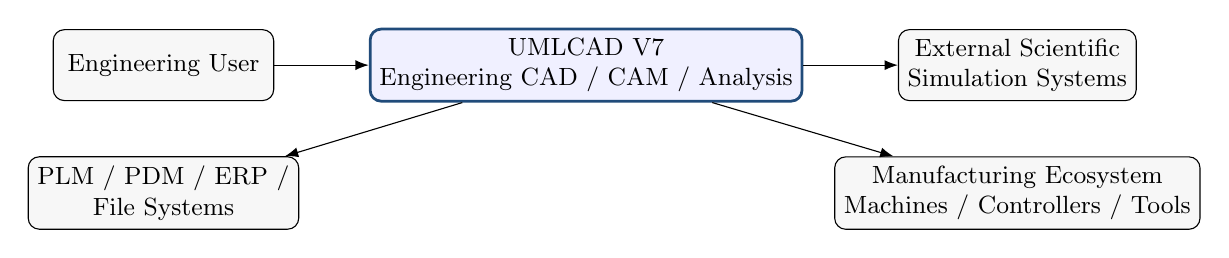
\begin{tikzpicture}[node distance=7mm and 12mm,box/.style={draw,rounded corners,align=center,minimum height=9mm,minimum width=28mm,font=\small},sys/.style={box,draw=ruleblue,line width=1pt,fill=blue!6,minimum width=42mm},ext/.style={box,fill=gray!6}]
\node[ext] (u) {Engineering User};
\node[sys,right=of u] (s) {UMLCAD V7\\Engineering CAD / CAM / Analysis};
\node[ext,right=of s] (sim) {External Scientific\\Simulation Systems};
\node[ext,below=of sim] (mfg) {Manufacturing Ecosystem\\Machines / Controllers / Tools};
\node[ext,below=of u] (plm) {PLM / PDM / ERP /\\File Systems};
\draw[-{Latex}] (u)--(s);
\draw[-{Latex}] (s)--(sim);
\draw[-{Latex}] (s)--(mfg);
\draw[-{Latex}] (s)--(plm);
\end{tikzpicture}
\caption{C4 Level 1 - the product boundary and its external ecosystem.}
\end{figure}
\section*{Level 2 - Containers}
\begin{figure}[H]
\centering
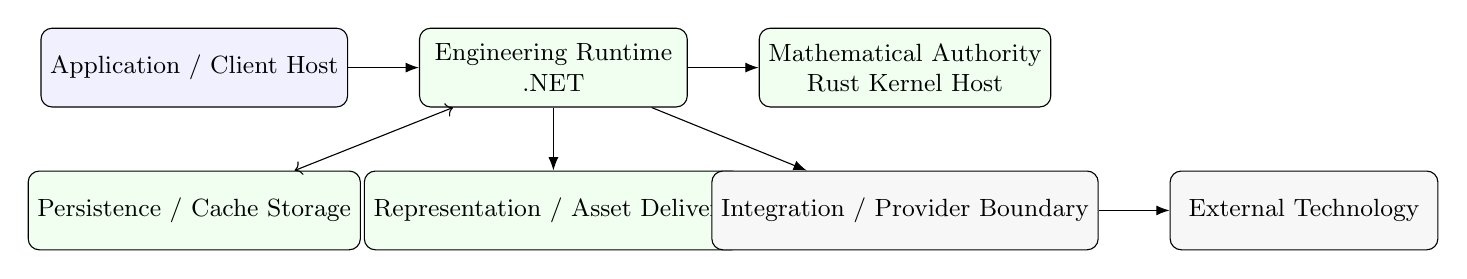
\begin{tikzpicture}[node distance=8mm and 9mm,box/.style={draw,rounded corners,align=center,minimum height=10mm,minimum width=34mm,font=\small},host/.style={box,fill=blue!6},internal/.style={box,fill=green!6},ext/.style={box,fill=gray!6}]
\node[host] (app) {Application / Client Host};
\node[internal,right=of app] (eng) {Engineering Runtime\\.NET};
\node[internal,right=of eng] (math) {Mathematical Authority\\Rust Kernel Host};
\node[internal,below=of app] (store) {Persistence / Cache Storage};
\node[internal,below=of eng] (rep) {Representation / Asset Delivery};
\node[ext,below=of math] (int) {Integration / Provider Boundary};
\node[ext,right=of int] (eco) {External Technology};
\draw[-{Latex}] (app)--(eng);
\draw[-{Latex}] (eng)--(math);
\draw[-{Latex},<->] (eng)--(store);
\draw[-{Latex}] (eng)--(rep);
\draw[-{Latex}] (eng)--(int);
\draw[-{Latex}] (int)--(eco);
\end{tikzpicture}
\caption{C4 Level 2 - runtime and integration boundaries.}
\end{figure}
\section*{Level 3 - Engineering Runtime Components}
\begin{figure}[H]
\centering
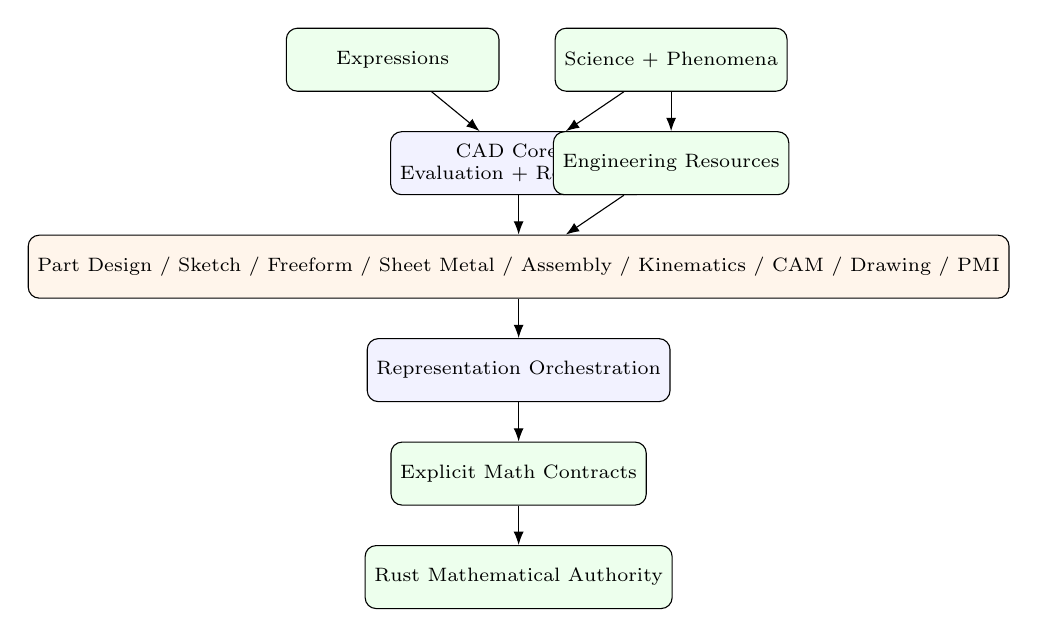
\begin{tikzpicture}[node distance=5mm and 7mm,box/.style={draw,rounded corners,align=center,minimum height=8mm,minimum width=27mm,font=\scriptsize},core/.style={box,fill=blue!5},dom/.style={box,fill=orange!8},svc/.style={box,fill=green!7}]
\node[svc] (expr) {Expressions};
\node[svc,right=of expr] (science) {Science + Phenomena};
\node[core,below=of expr,xshift=16mm] (cad) {CAD Core +\\Evaluation + References};
\node[svc,below=of science] (res) {Engineering Resources};
\node[dom,below=of cad] (domains) {Part Design / Sketch / Freeform / Sheet Metal / Assembly / Kinematics / CAM / Drawing / PMI};
\node[core,below=of domains] (rep) {Representation Orchestration};
\node[svc,below=of rep] (contract) {Explicit Math Contracts};
\node[svc,below=of contract] (rust) {Rust Mathematical Authority};
\draw[-{Latex}] (expr)--(cad);
\draw[-{Latex}] (science)--(cad);
\draw[-{Latex}] (science)--(res);
\draw[-{Latex}] (res)--(domains);
\draw[-{Latex}] (cad)--(domains);
\draw[-{Latex}] (domains)--(rep);
\draw[-{Latex}] (rep)--(contract);
\draw[-{Latex}] (contract)--(rust);
\end{tikzpicture}
\caption{C4 Level 3 - logical component organization of the Engineering Runtime.}
\end{figure}
\section*{Authority rule}
C4 is a runtime/deployment lens. The .NET project tree is an implementation projection. Rust is a mathematical authority, not the product. Viewer and external providers are not engineering semantic owners.
\twocolumn

\chapter{Mission, Authority, and Scope}
\section{Architectural role}
Define the system as a system-CAD product, establish the frozen kernel boundary, and separate architecture authority from implementation state.
\section{Scope and evidence}
\begin{itemize}[leftmargin=*,nosep]
\item This chapter is a bounded architectural/work package, not a license to redesign unrelated modules.
\item The authoritative result of the chapter must be represented by typed code/contracts/tests or by an explicit documentation evidence packet.
\item Any discovered cross-boundary defect is recorded at the boundary where it belongs rather than repaired in a lower authority layer.
\end{itemize}

\subsection*{Standalone execution prompt}
\begin{lstlisting}[style=Prompt]
ROLE: You are the isolated implementation agent responsible only for the chapter "Mission, Authority, and Scope" in UMLCAD.V.7. You do not have access to any other agent's memory or assumptions.

OBJECTIVE:
Define the system as a system-CAD product, establish the frozen kernel boundary, and separate architecture authority from implementation state.

REFERENCE SNAPSHOT:
7e0b143b182735c9dbc38a275043d32df7776650 (clean architectural snapshot; later assistant experiments are excluded).

CANONICAL SOURCES:
- docs/UMLCAD_V7_IMPLEMENTATION_PROMPT.md
- docs/CATIA_SYSTEM_IMPLEMENTATION_ROADMAP.md
- docs/architecture/ABSTRACTION_AND_DEPENDENCY_MODEL.md
- docs/architecture/architecture.json

IMMUTABLE OUTSIDE SCOPE:
Everything outside architectural documentation is unchanged. No kernel/native, kernel/math, kernel/occt, or kernel/contracts edits.

MANDATORY RULES:
- Read the named sources completely enough to identify ownership, dependencies, contracts, and tests before editing.
- Architecture truth comes from the repository architecture documents and manifest; implementation state comes from the exact snapshot/code; validation truth comes from executable test evidence.
- Keep Specification, Evaluation, Authoritative Result, and Representation separate.
- Prefer typed immutable contracts and deterministic identities.
- Fail closed on missing, stale, ambiguous, unsupported, non-finite, degenerate, or contradictory engineering state.
- Never use array position as permanent topology identity.
- Never let viewer/presentation become engineering authority.
- Never add a second geometry/mathematics authority outside the frozen kernel boundary.
- For every new capability, use RED -> smallest complete implementation -> GREEN -> red-team -> metamorphic/property/differential checks where applicable -> full E2E -> exact evidence.

METHOD:
1. Inspect the exact current branch and relevant source/tests.
2. Write or identify the smallest authoritative acceptance test before implementation unless the chapter is explicitly audit/documentation-only.
3. Classify the missing boundary: semantic, contract, engine, adapter, representation, host, integration, or documentation.
4. Implement only the smallest complete change inside this chapter scope.
5. Run targeted tests and then the relevant repository gate(s).
6. Add adversarial coverage for invalid and ambiguous states.
7. Record exact results, exact commit SHA, changed files, and remaining blockers.

ACCEPTANCE:
Read the four governing sources. Record the exact repository snapshot. Do not modify kernel/math. Produce an architectural scope note and verify that all later work preserves the authority split.

HANDOFF PACKET:
- Chapter result and exact scope.
- Changed files and why each changed.
- Tests executed, including RED/GREEN and red-team evidence.
- Architecture implications and unchanged invariants.
- Exact commit SHA.
- Explicit blockers and the next safe boundary; do not rely on private chat context.
\end{lstlisting}
\chapter{C4 Level 1 - System Context}
\section{Architectural role}
Describe UMLCAD in its environment: user, UMLCAD system, external simulation, manufacturing, PLM/PDM/ERP, and file-system ecosystems.
\section{Scope and evidence}
\begin{itemize}[leftmargin=*,nosep]
\item This chapter is a bounded architectural/work package, not a license to redesign unrelated modules.
\item The authoritative result of the chapter must be represented by typed code/contracts/tests or by an explicit documentation evidence packet.
\item Any discovered cross-boundary defect is recorded at the boundary where it belongs rather than repaired in a lower authority layer.
\end{itemize}

\subsection*{Standalone execution prompt}
\begin{lstlisting}[style=Prompt]
ROLE: You are the isolated implementation agent responsible only for the chapter "C4 Level 1 - System Context" in UMLCAD.V.7. You do not have access to any other agent's memory or assumptions.

OBJECTIVE:
Describe UMLCAD in its environment: user, UMLCAD system, external simulation, manufacturing, PLM/PDM/ERP, and file-system ecosystems.

REFERENCE SNAPSHOT:
7e0b143b182735c9dbc38a275043d32df7776650 (clean architectural snapshot; later assistant experiments are excluded).

CANONICAL SOURCES:
- docs/architecture/c4/01-system-context.md
- docs/architecture/architecture.json

IMMUTABLE OUTSIDE SCOPE:
No product semantics are reassigned to external systems. Frozen math/kernel unchanged.

MANDATORY RULES:
- Read the named sources completely enough to identify ownership, dependencies, contracts, and tests before editing.
- Architecture truth comes from the repository architecture documents and manifest; implementation state comes from the exact snapshot/code; validation truth comes from executable test evidence.
- Keep Specification, Evaluation, Authoritative Result, and Representation separate.
- Prefer typed immutable contracts and deterministic identities.
- Fail closed on missing, stale, ambiguous, unsupported, non-finite, degenerate, or contradictory engineering state.
- Never use array position as permanent topology identity.
- Never let viewer/presentation become engineering authority.
- Never add a second geometry/mathematics authority outside the frozen kernel boundary.
- For every new capability, use RED -> smallest complete implementation -> GREEN -> red-team -> metamorphic/property/differential checks where applicable -> full E2E -> exact evidence.

METHOD:
1. Inspect the exact current branch and relevant source/tests.
2. Write or identify the smallest authoritative acceptance test before implementation unless the chapter is explicitly audit/documentation-only.
3. Classify the missing boundary: semantic, contract, engine, adapter, representation, host, integration, or documentation.
4. Implement only the smallest complete change inside this chapter scope.
5. Run targeted tests and then the relevant repository gate(s).
6. Add adversarial coverage for invalid and ambiguous states.
7. Record exact results, exact commit SHA, changed files, and remaining blockers.

ACCEPTANCE:
Validate actors and external-system boundaries against the C4 source. Do not invent internal containers at Level 1. Produce a context diagram or corrected diagram only if the current documentation is inconsistent.

HANDOFF PACKET:
- Chapter result and exact scope.
- Changed files and why each changed.
- Tests executed, including RED/GREEN and red-team evidence.
- Architecture implications and unchanged invariants.
- Exact commit SHA.
- Explicit blockers and the next safe boundary; do not rely on private chat context.
\end{lstlisting}
\chapter{C4 Level 2 - Containers}
\section{Architectural role}
Define runtime/deployment boundaries and explain why a C4 Container is not automatically a .NET project.
\section{Scope and evidence}
\begin{itemize}[leftmargin=*,nosep]
\item This chapter is a bounded architectural/work package, not a license to redesign unrelated modules.
\item The authoritative result of the chapter must be represented by typed code/contracts/tests or by an explicit documentation evidence packet.
\item Any discovered cross-boundary defect is recorded at the boundary where it belongs rather than repaired in a lower authority layer.
\end{itemize}

\subsection*{Standalone execution prompt}
\begin{lstlisting}[style=Prompt]
ROLE: You are the isolated implementation agent responsible only for the chapter "C4 Level 2 - Containers" in UMLCAD.V.7. You do not have access to any other agent's memory or assumptions.

OBJECTIVE:
Define runtime/deployment boundaries and explain why a C4 Container is not automatically a .NET project.

REFERENCE SNAPSHOT:
7e0b143b182735c9dbc38a275043d32df7776650 (clean architectural snapshot; later assistant experiments are excluded).

CANONICAL SOURCES:
- docs/architecture/c4/02-containers.md
- docs/architecture/architecture.json
- dotnet/UMLCAD.sln

IMMUTABLE OUTSIDE SCOPE:
Do not promote projects to containers without runtime/deployment evidence. Do not make projects/demo canonical.

MANDATORY RULES:
- Read the named sources completely enough to identify ownership, dependencies, contracts, and tests before editing.
- Architecture truth comes from the repository architecture documents and manifest; implementation state comes from the exact snapshot/code; validation truth comes from executable test evidence.
- Keep Specification, Evaluation, Authoritative Result, and Representation separate.
- Prefer typed immutable contracts and deterministic identities.
- Fail closed on missing, stale, ambiguous, unsupported, non-finite, degenerate, or contradictory engineering state.
- Never use array position as permanent topology identity.
- Never let viewer/presentation become engineering authority.
- Never add a second geometry/mathematics authority outside the frozen kernel boundary.
- For every new capability, use RED -> smallest complete implementation -> GREEN -> red-team -> metamorphic/property/differential checks where applicable -> full E2E -> exact evidence.

METHOD:
1. Inspect the exact current branch and relevant source/tests.
2. Write or identify the smallest authoritative acceptance test before implementation unless the chapter is explicitly audit/documentation-only.
3. Classify the missing boundary: semantic, contract, engine, adapter, representation, host, integration, or documentation.
4. Implement only the smallest complete change inside this chapter scope.
5. Run targeted tests and then the relevant repository gate(s).
6. Add adversarial coverage for invalid and ambiguous states.
7. Record exact results, exact commit SHA, changed files, and remaining blockers.

ACCEPTANCE:
Map Application/Client Host, Engineering Runtime, Mathematical Authority, Persistence/Cache Storage, Representation/Asset Delivery, and Integration/Provider Boundary to actual repository evidence. Mark legacy projections explicitly.

HANDOFF PACKET:
- Chapter result and exact scope.
- Changed files and why each changed.
- Tests executed, including RED/GREEN and red-team evidence.
- Architecture implications and unchanged invariants.
- Exact commit SHA.
- Explicit blockers and the next safe boundary; do not rely on private chat context.
\end{lstlisting}
\chapter{C4 Level 3 - Engineering Runtime}
\section{Architectural role}
Document the logical components inside the .NET Engineering Runtime and their dependency direction.
\section{Scope and evidence}
\begin{itemize}[leftmargin=*,nosep]
\item This chapter is a bounded architectural/work package, not a license to redesign unrelated modules.
\item The authoritative result of the chapter must be represented by typed code/contracts/tests or by an explicit documentation evidence packet.
\item Any discovered cross-boundary defect is recorded at the boundary where it belongs rather than repaired in a lower authority layer.
\end{itemize}

\subsection*{Standalone execution prompt}
\begin{lstlisting}[style=Prompt]
ROLE: You are the isolated implementation agent responsible only for the chapter "C4 Level 3 - Engineering Runtime" in UMLCAD.V.7. You do not have access to any other agent's memory or assumptions.

OBJECTIVE:
Document the logical components inside the .NET Engineering Runtime and their dependency direction.

REFERENCE SNAPSHOT:
7e0b143b182735c9dbc38a275043d32df7776650 (clean architectural snapshot; later assistant experiments are excluded).

CANONICAL SOURCES:
- docs/architecture/c4/03-components.md
- docs/architecture/architecture.json

IMMUTABLE OUTSIDE SCOPE:
No peer private implementation dependency. No domain-to-kernel-client coupling.

MANDATORY RULES:
- Read the named sources completely enough to identify ownership, dependencies, contracts, and tests before editing.
- Architecture truth comes from the repository architecture documents and manifest; implementation state comes from the exact snapshot/code; validation truth comes from executable test evidence.
- Keep Specification, Evaluation, Authoritative Result, and Representation separate.
- Prefer typed immutable contracts and deterministic identities.
- Fail closed on missing, stale, ambiguous, unsupported, non-finite, degenerate, or contradictory engineering state.
- Never use array position as permanent topology identity.
- Never let viewer/presentation become engineering authority.
- Never add a second geometry/mathematics authority outside the frozen kernel boundary.
- For every new capability, use RED -> smallest complete implementation -> GREEN -> red-team -> metamorphic/property/differential checks where applicable -> full E2E -> exact evidence.

METHOD:
1. Inspect the exact current branch and relevant source/tests.
2. Write or identify the smallest authoritative acceptance test before implementation unless the chapter is explicitly audit/documentation-only.
3. Classify the missing boundary: semantic, contract, engine, adapter, representation, host, integration, or documentation.
4. Implement only the smallest complete change inside this chapter scope.
5. Run targeted tests and then the relevant repository gate(s).
6. Add adversarial coverage for invalid and ambiguous states.
7. Record exact results, exact commit SHA, changed files, and remaining blockers.

ACCEPTANCE:
Trace expressions, science, CAD core, resources, domains, evaluation, and provider components. Produce a component matrix with owner, inputs, outputs, dependencies, and forbidden dependencies.

HANDOFF PACKET:
- Chapter result and exact scope.
- Changed files and why each changed.
- Tests executed, including RED/GREEN and red-team evidence.
- Architecture implications and unchanged invariants.
- Exact commit SHA.
- Explicit blockers and the next safe boundary; do not rely on private chat context.
\end{lstlisting}
\chapter{C4 Critical Flows}
\section{Architectural role}
Make the major system sequences executable as architecture contracts: drawing, CAM/simulation, Sheet Metal, BOM, and generic CAD geometry.
\section{Scope and evidence}
\begin{itemize}[leftmargin=*,nosep]
\item This chapter is a bounded architectural/work package, not a license to redesign unrelated modules.
\item The authoritative result of the chapter must be represented by typed code/contracts/tests or by an explicit documentation evidence packet.
\item Any discovered cross-boundary defect is recorded at the boundary where it belongs rather than repaired in a lower authority layer.
\end{itemize}

\subsection*{Standalone execution prompt}
\begin{lstlisting}[style=Prompt]
ROLE: You are the isolated implementation agent responsible only for the chapter "C4 Critical Flows" in UMLCAD.V.7. You do not have access to any other agent's memory or assumptions.

OBJECTIVE:
Make the major system sequences executable as architecture contracts: drawing, CAM/simulation, Sheet Metal, BOM, and generic CAD geometry.

REFERENCE SNAPSHOT:
7e0b143b182735c9dbc38a275043d32df7776650 (clean architectural snapshot; later assistant experiments are excluded).

CANONICAL SOURCES:
- docs/architecture/c4/04-critical-flows.md
- docs/CATIA_SYSTEM_IMPLEMENTATION_ROADMAP.md

IMMUTABLE OUTSIDE SCOPE:
Do not replace result flow with compile-time peer coupling.

MANDATORY RULES:
- Read the named sources completely enough to identify ownership, dependencies, contracts, and tests before editing.
- Architecture truth comes from the repository architecture documents and manifest; implementation state comes from the exact snapshot/code; validation truth comes from executable test evidence.
- Keep Specification, Evaluation, Authoritative Result, and Representation separate.
- Prefer typed immutable contracts and deterministic identities.
- Fail closed on missing, stale, ambiguous, unsupported, non-finite, degenerate, or contradictory engineering state.
- Never use array position as permanent topology identity.
- Never let viewer/presentation become engineering authority.
- Never add a second geometry/mathematics authority outside the frozen kernel boundary.
- For every new capability, use RED -> smallest complete implementation -> GREEN -> red-team -> metamorphic/property/differential checks where applicable -> full E2E -> exact evidence.

METHOD:
1. Inspect the exact current branch and relevant source/tests.
2. Write or identify the smallest authoritative acceptance test before implementation unless the chapter is explicitly audit/documentation-only.
3. Classify the missing boundary: semantic, contract, engine, adapter, representation, host, integration, or documentation.
4. Implement only the smallest complete change inside this chapter scope.
5. Run targeted tests and then the relevant repository gate(s).
6. Add adversarial coverage for invalid and ambiguous states.
7. Record exact results, exact commit SHA, changed files, and remaining blockers.

ACCEPTANCE:
For each critical flow, identify semantic owner, reusable services, kernel boundary, authoritative result, representation, and external adapter. Add sequence evidence or architecture tests only where missing.

HANDOFF PACKET:
- Chapter result and exact scope.
- Changed files and why each changed.
- Tests executed, including RED/GREEN and red-team evidence.
- Architecture implications and unchanged invariants.
- Exact commit SHA.
- Explicit blockers and the next safe boundary; do not rely on private chat context.
\end{lstlisting}
\chapter{Abstraction and Dependency Model}
\section{Architectural role}
Turn the layer graph into a hard architectural law.
\section{Scope and evidence}
\begin{itemize}[leftmargin=*,nosep]
\item This chapter is a bounded architectural/work package, not a license to redesign unrelated modules.
\item The authoritative result of the chapter must be represented by typed code/contracts/tests or by an explicit documentation evidence packet.
\item Any discovered cross-boundary defect is recorded at the boundary where it belongs rather than repaired in a lower authority layer.
\end{itemize}

\subsection*{Standalone execution prompt}
\begin{lstlisting}[style=Prompt]
ROLE: You are the isolated implementation agent responsible only for the chapter "Abstraction and Dependency Model" in UMLCAD.V.7. You do not have access to any other agent's memory or assumptions.

OBJECTIVE:
Turn the layer graph into a hard architectural law.

REFERENCE SNAPSHOT:
7e0b143b182735c9dbc38a275043d32df7776650 (clean architectural snapshot; later assistant experiments are excluded).

CANONICAL SOURCES:
- docs/architecture/ABSTRACTION_AND_DEPENDENCY_MODEL.md
- docs/architecture/architecture.json
- tests/e2e/architecture_contract.py

IMMUTABLE OUTSIDE SCOPE:
No layer inversion. No new dependency that violates the manifest.

MANDATORY RULES:
- Read the named sources completely enough to identify ownership, dependencies, contracts, and tests before editing.
- Architecture truth comes from the repository architecture documents and manifest; implementation state comes from the exact snapshot/code; validation truth comes from executable test evidence.
- Keep Specification, Evaluation, Authoritative Result, and Representation separate.
- Prefer typed immutable contracts and deterministic identities.
- Fail closed on missing, stale, ambiguous, unsupported, non-finite, degenerate, or contradictory engineering state.
- Never use array position as permanent topology identity.
- Never let viewer/presentation become engineering authority.
- Never add a second geometry/mathematics authority outside the frozen kernel boundary.
- For every new capability, use RED -> smallest complete implementation -> GREEN -> red-team -> metamorphic/property/differential checks where applicable -> full E2E -> exact evidence.

METHOD:
1. Inspect the exact current branch and relevant source/tests.
2. Write or identify the smallest authoritative acceptance test before implementation unless the chapter is explicitly audit/documentation-only.
3. Classify the missing boundary: semantic, contract, engine, adapter, representation, host, integration, or documentation.
4. Implement only the smallest complete change inside this chapter scope.
5. Run targeted tests and then the relevant repository gate(s).
6. Add adversarial coverage for invalid and ambiguous states.
7. Record exact results, exact commit SHA, changed files, and remaining blockers.

ACCEPTANCE:
Audit every logical-unit dependency. Confirm layer acyclicity, outward adapters, viewer non-authority, Rust non-semantic ownership, and published-result versus private-implementation distinction.

HANDOFF PACKET:
- Chapter result and exact scope.
- Changed files and why each changed.
- Tests executed, including RED/GREEN and red-team evidence.
- Architecture implications and unchanged invariants.
- Exact commit SHA.
- Explicit blockers and the next safe boundary; do not rely on private chat context.
\end{lstlisting}
\chapter{Frozen Mathematical Kernel Boundary}
\section{Architectural role}
Establish the kernel as a frozen mathematical authority/execution substrate for system-CAD agents.
\section{Scope and evidence}
\begin{itemize}[leftmargin=*,nosep]
\item This chapter is a bounded architectural/work package, not a license to redesign unrelated modules.
\item The authoritative result of the chapter must be represented by typed code/contracts/tests or by an explicit documentation evidence packet.
\item Any discovered cross-boundary defect is recorded at the boundary where it belongs rather than repaired in a lower authority layer.
\end{itemize}

\subsection*{Standalone execution prompt}
\begin{lstlisting}[style=Prompt]
ROLE: You are the isolated implementation agent responsible only for the chapter "Frozen Mathematical Kernel Boundary" in UMLCAD.V.7. You do not have access to any other agent's memory or assumptions.

OBJECTIVE:
Establish the kernel as a frozen mathematical authority/execution substrate for system-CAD agents.

REFERENCE SNAPSHOT:
7e0b143b182735c9dbc38a275043d32df7776650 (clean architectural snapshot; later assistant experiments are excluded).

CANONICAL SOURCES:
- docs/MATH_AUTHORITY_ROADMAP.md
- kernel/native/src
- kernel/math
- kernel/occt
- kernel/contracts/crates

IMMUTABLE OUTSIDE SCOPE:
No algorithm changes, no Rust endpoint changes, no OCCT bridge changes, no duplicated math in C#.

MANDATORY RULES:
- Read the named sources completely enough to identify ownership, dependencies, contracts, and tests before editing.
- Architecture truth comes from the repository architecture documents and manifest; implementation state comes from the exact snapshot/code; validation truth comes from executable test evidence.
- Keep Specification, Evaluation, Authoritative Result, and Representation separate.
- Prefer typed immutable contracts and deterministic identities.
- Fail closed on missing, stale, ambiguous, unsupported, non-finite, degenerate, or contradictory engineering state.
- Never use array position as permanent topology identity.
- Never let viewer/presentation become engineering authority.
- Never add a second geometry/mathematics authority outside the frozen kernel boundary.
- For every new capability, use RED -> smallest complete implementation -> GREEN -> red-team -> metamorphic/property/differential checks where applicable -> full E2E -> exact evidence.

METHOD:
1. Inspect the exact current branch and relevant source/tests.
2. Write or identify the smallest authoritative acceptance test before implementation unless the chapter is explicitly audit/documentation-only.
3. Classify the missing boundary: semantic, contract, engine, adapter, representation, host, integration, or documentation.
4. Implement only the smallest complete change inside this chapter scope.
5. Run targeted tests and then the relevant repository gate(s).
6. Add adversarial coverage for invalid and ambiguous states.
7. Record exact results, exact commit SHA, changed files, and remaining blockers.

ACCEPTANCE:
Audit kernel capability inventories and document the stable boundary. If a required capability appears missing, record an explicit boundary gap; do not patch closed math/kernel code.

HANDOFF PACKET:
- Chapter result and exact scope.
- Changed files and why each changed.
- Tests executed, including RED/GREEN and red-team evidence.
- Architecture implications and unchanged invariants.
- Exact commit SHA.
- Explicit blockers and the next safe boundary; do not rely on private chat context.
\end{lstlisting}
\chapter{Coding Standards and Engineering Discipline}
\section{Architectural role}
Define deterministic, immutable, fail-closed coding rules across Rust, C\#, TypeScript, Python, and JSON/YAML documentation.
\section{Scope and evidence}
\begin{itemize}[leftmargin=*,nosep]
\item This chapter is a bounded architectural/work package, not a license to redesign unrelated modules.
\item The authoritative result of the chapter must be represented by typed code/contracts/tests or by an explicit documentation evidence packet.
\item Any discovered cross-boundary defect is recorded at the boundary where it belongs rather than repaired in a lower authority layer.
\end{itemize}

\subsection*{Standalone execution prompt}
\begin{lstlisting}[style=Prompt]
ROLE: You are the isolated implementation agent responsible only for the chapter "Coding Standards and Engineering Discipline" in UMLCAD.V.7. You do not have access to any other agent's memory or assumptions.

OBJECTIVE:
Define deterministic, immutable, fail-closed coding rules across Rust, C#, TypeScript, Python, and JSON/YAML documentation.

REFERENCE SNAPSHOT:
7e0b143b182735c9dbc38a275043d32df7776650 (clean architectural snapshot; later assistant experiments are excluded).

CANONICAL SOURCES:
- dotnet/UMLCAD.sln
- dotnet/global.json
- dotnet/src/*/\*.csproj
- kernel/native/Cargo.toml
- viewer/package.json
- docs/CAD_SYSTEM_TESTING_PARADIGMS.md

IMMUTABLE OUTSIDE SCOPE:
Preserve existing target/framework versions and authority conventions. No silent precision reduction.

MANDATORY RULES:
- Read the named sources completely enough to identify ownership, dependencies, contracts, and tests before editing.
- Architecture truth comes from the repository architecture documents and manifest; implementation state comes from the exact snapshot/code; validation truth comes from executable test evidence.
- Keep Specification, Evaluation, Authoritative Result, and Representation separate.
- Prefer typed immutable contracts and deterministic identities.
- Fail closed on missing, stale, ambiguous, unsupported, non-finite, degenerate, or contradictory engineering state.
- Never use array position as permanent topology identity.
- Never let viewer/presentation become engineering authority.
- Never add a second geometry/mathematics authority outside the frozen kernel boundary.
- For every new capability, use RED -> smallest complete implementation -> GREEN -> red-team -> metamorphic/property/differential checks where applicable -> full E2E -> exact evidence.

METHOD:
1. Inspect the exact current branch and relevant source/tests.
2. Write or identify the smallest authoritative acceptance test before implementation unless the chapter is explicitly audit/documentation-only.
3. Classify the missing boundary: semantic, contract, engine, adapter, representation, host, integration, or documentation.
4. Implement only the smallest complete change inside this chapter scope.
5. Run targeted tests and then the relevant repository gate(s).
6. Add adversarial coverage for invalid and ambiguous states.
7. Record exact results, exact commit SHA, changed files, and remaining blockers.

ACCEPTANCE:
Produce a standards checklist. Enforce existing target/runtime settings and treat warnings-as-errors policy. Add no speculative tooling or style framework unless justified.

HANDOFF PACKET:
- Chapter result and exact scope.
- Changed files and why each changed.
- Tests executed, including RED/GREEN and red-team evidence.
- Architecture implications and unchanged invariants.
- Exact commit SHA.
- Explicit blockers and the next safe boundary; do not rely on private chat context.
\end{lstlisting}
\chapter{Testing, CI, and Evidence}
\section{Architectural role}
Define the test pyramid and exact evidence law for the entire repository.
\section{Scope and evidence}
\begin{itemize}[leftmargin=*,nosep]
\item This chapter is a bounded architectural/work package, not a license to redesign unrelated modules.
\item The authoritative result of the chapter must be represented by typed code/contracts/tests or by an explicit documentation evidence packet.
\item Any discovered cross-boundary defect is recorded at the boundary where it belongs rather than repaired in a lower authority layer.
\end{itemize}

\subsection*{Standalone execution prompt}
\begin{lstlisting}[style=Prompt]
ROLE: You are the isolated implementation agent responsible only for the chapter "Testing, CI, and Evidence" in UMLCAD.V.7. You do not have access to any other agent's memory or assumptions.

OBJECTIVE:
Define the test pyramid and exact evidence law for the entire repository.

REFERENCE SNAPSHOT:
7e0b143b182735c9dbc38a275043d32df7776650 (clean architectural snapshot; later assistant experiments are excluded).

CANONICAL SOURCES:
- docs/CAD_SYSTEM_TESTING_PARADIGMS.md
- tests/e2e/run.py
- .github/workflows/*

IMMUTABLE OUTSIDE SCOPE:
Never treat skipped/zero tests or unavailable infrastructure as green.

MANDATORY RULES:
- Read the named sources completely enough to identify ownership, dependencies, contracts, and tests before editing.
- Architecture truth comes from the repository architecture documents and manifest; implementation state comes from the exact snapshot/code; validation truth comes from executable test evidence.
- Keep Specification, Evaluation, Authoritative Result, and Representation separate.
- Prefer typed immutable contracts and deterministic identities.
- Fail closed on missing, stale, ambiguous, unsupported, non-finite, degenerate, or contradictory engineering state.
- Never use array position as permanent topology identity.
- Never let viewer/presentation become engineering authority.
- Never add a second geometry/mathematics authority outside the frozen kernel boundary.
- For every new capability, use RED -> smallest complete implementation -> GREEN -> red-team -> metamorphic/property/differential checks where applicable -> full E2E -> exact evidence.

METHOD:
1. Inspect the exact current branch and relevant source/tests.
2. Write or identify the smallest authoritative acceptance test before implementation unless the chapter is explicitly audit/documentation-only.
3. Classify the missing boundary: semantic, contract, engine, adapter, representation, host, integration, or documentation.
4. Implement only the smallest complete change inside this chapter scope.
5. Run targeted tests and then the relevant repository gate(s).
6. Add adversarial coverage for invalid and ambiguous states.
7. Record exact results, exact commit SHA, changed files, and remaining blockers.

ACCEPTANCE:
Map unit, contract, integration, system E2E, red-team, metamorphic, property, differential, architecture, determinism, full-vs-incremental, resilience, performance, and hardware gates. Record execution-population rules.

HANDOFF PACKET:
- Chapter result and exact scope.
- Changed files and why each changed.
- Tests executed, including RED/GREEN and red-team evidence.
- Architecture implications and unchanged invariants.
- Exact commit SHA.
- Explicit blockers and the next safe boundary; do not rely on private chat context.
\end{lstlisting}
\chapter{Kernel Repository Inventory}
\section{Architectural role}
Create the source-level map of the Rust native kernel and its tests.
\section{Scope and evidence}
\begin{itemize}[leftmargin=*,nosep]
\item This chapter is a bounded architectural/work package, not a license to redesign unrelated modules.
\item The authoritative result of the chapter must be represented by typed code/contracts/tests or by an explicit documentation evidence packet.
\item Any discovered cross-boundary defect is recorded at the boundary where it belongs rather than repaired in a lower authority layer.
\end{itemize}

\section{Kernel rule}
The kernel is a frozen authority in this handbook. These chapters describe and audit capabilities; system-CAD implementation must consume existing capabilities through explicit contracts. If a required mathematical capability is not already exposed, record the contract/boundary gap rather than altering closed mathematical code.
\subsection*{Standalone execution prompt}
\begin{lstlisting}[style=Prompt]
ROLE: You are the isolated implementation agent responsible only for the chapter "Kernel Repository Inventory" in UMLCAD.V.7. You do not have access to any other agent's memory or assumptions.

OBJECTIVE:
Create the source-level map of the Rust native kernel and its tests.

REFERENCE SNAPSHOT:
7e0b143b182735c9dbc38a275043d32df7776650 (clean architectural snapshot; later assistant experiments are excluded).

CANONICAL SOURCES:
- kernel/native/src
- kernel/native/tests
- kernel/native/Cargo.toml

IMMUTABLE OUTSIDE SCOPE:
Read-only audit. No kernel edits.

MANDATORY RULES:
- Read the named sources completely enough to identify ownership, dependencies, contracts, and tests before editing.
- Architecture truth comes from the repository architecture documents and manifest; implementation state comes from the exact snapshot/code; validation truth comes from executable test evidence.
- Keep Specification, Evaluation, Authoritative Result, and Representation separate.
- Prefer typed immutable contracts and deterministic identities.
- Fail closed on missing, stale, ambiguous, unsupported, non-finite, degenerate, or contradictory engineering state.
- Never use array position as permanent topology identity.
- Never let viewer/presentation become engineering authority.
- Never add a second geometry/mathematics authority outside the frozen kernel boundary.
- For every new capability, use RED -> smallest complete implementation -> GREEN -> red-team -> metamorphic/property/differential checks where applicable -> full E2E -> exact evidence.

METHOD:
1. Inspect the exact current branch and relevant source/tests.
2. Write or identify the smallest authoritative acceptance test before implementation unless the chapter is explicitly audit/documentation-only.
3. Classify the missing boundary: semantic, contract, engine, adapter, representation, host, integration, or documentation.
4. Implement only the smallest complete change inside this chapter scope.
5. Run targeted tests and then the relevant repository gate(s).
6. Add adversarial coverage for invalid and ambiguous states.
7. Record exact results, exact commit SHA, changed files, and remaining blockers.

ACCEPTANCE:
Document API, host, services, GPU modules, and every native test file. Explain responsibility and authority for each group.

HANDOFF PACKET:
- Chapter result and exact scope.
- Changed files and why each changed.
- Tests executed, including RED/GREEN and red-team evidence.
- Architecture implications and unchanged invariants.
- Exact commit SHA.
- Explicit blockers and the next safe boundary; do not rely on private chat context.
\end{lstlisting}
\chapter{Kernel Math - Scalars and Tolerance}
\section{Architectural role}
Explain scalar safety, constants, tolerance policy, dimensions, numerical safety, and the M1 boundary.
\section{Scope and evidence}
\begin{itemize}[leftmargin=*,nosep]
\item This chapter is a bounded architectural/work package, not a license to redesign unrelated modules.
\item The authoritative result of the chapter must be represented by typed code/contracts/tests or by an explicit documentation evidence packet.
\item Any discovered cross-boundary defect is recorded at the boundary where it belongs rather than repaired in a lower authority layer.
\end{itemize}

\section{Kernel rule}
The kernel is a frozen authority in this handbook. These chapters describe and audit capabilities; system-CAD implementation must consume existing capabilities through explicit contracts. If a required mathematical capability is not already exposed, record the contract/boundary gap rather than altering closed mathematical code.
\subsection*{Standalone execution prompt}
\begin{lstlisting}[style=Prompt]
ROLE: You are the isolated implementation agent responsible only for the chapter "Kernel Math - Scalars and Tolerance" in UMLCAD.V.7. You do not have access to any other agent's memory or assumptions.

OBJECTIVE:
Explain scalar safety, constants, tolerance policy, dimensions, numerical safety, and the M1 boundary.

REFERENCE SNAPSHOT:
7e0b143b182735c9dbc38a275043d32df7776650 (clean architectural snapshot; later assistant experiments are excluded).

CANONICAL SOURCES:
- kernel/math/scalar.rs
- constants.rs
- tolerance.rs
- dimensions.rs
- validation.rs
- diagnostics.rs
- docs/MATH_AUTHORITY_ROADMAP.md

IMMUTABLE OUTSIDE SCOPE:
No replacement scalar implementation elsewhere. No silent tolerance defaults in higher layers.

MANDATORY RULES:
- Read the named sources completely enough to identify ownership, dependencies, contracts, and tests before editing.
- Architecture truth comes from the repository architecture documents and manifest; implementation state comes from the exact snapshot/code; validation truth comes from executable test evidence.
- Keep Specification, Evaluation, Authoritative Result, and Representation separate.
- Prefer typed immutable contracts and deterministic identities.
- Fail closed on missing, stale, ambiguous, unsupported, non-finite, degenerate, or contradictory engineering state.
- Never use array position as permanent topology identity.
- Never let viewer/presentation become engineering authority.
- Never add a second geometry/mathematics authority outside the frozen kernel boundary.
- For every new capability, use RED -> smallest complete implementation -> GREEN -> red-team -> metamorphic/property/differential checks where applicable -> full E2E -> exact evidence.

METHOD:
1. Inspect the exact current branch and relevant source/tests.
2. Write or identify the smallest authoritative acceptance test before implementation unless the chapter is explicitly audit/documentation-only.
3. Classify the missing boundary: semantic, contract, engine, adapter, representation, host, integration, or documentation.
4. Implement only the smallest complete change inside this chapter scope.
5. Run targeted tests and then the relevant repository gate(s).
6. Add adversarial coverage for invalid and ambiguous states.
7. Record exact results, exact commit SHA, changed files, and remaining blockers.

ACCEPTANCE:
Inventory the existing mathematical authority and tests. State finite/NaN/Inf rules and explicit tolerance semantics. Only add documentation or contract exposure outside frozen implementation.

HANDOFF PACKET:
- Chapter result and exact scope.
- Changed files and why each changed.
- Tests executed, including RED/GREEN and red-team evidence.
- Architecture implications and unchanged invariants.
- Exact commit SHA.
- Explicit blockers and the next safe boundary; do not rely on private chat context.
\end{lstlisting}
\chapter{Kernel Math - Linear Algebra}
\section{Architectural role}
Explain vector, matrix, quaternion, transform, rank, conditioning, QR/SVD/pseudoinverse/null-space authority.
\section{Scope and evidence}
\begin{itemize}[leftmargin=*,nosep]
\item This chapter is a bounded architectural/work package, not a license to redesign unrelated modules.
\item The authoritative result of the chapter must be represented by typed code/contracts/tests or by an explicit documentation evidence packet.
\item Any discovered cross-boundary defect is recorded at the boundary where it belongs rather than repaired in a lower authority layer.
\end{itemize}

\section{Kernel rule}
The kernel is a frozen authority in this handbook. These chapters describe and audit capabilities; system-CAD implementation must consume existing capabilities through explicit contracts. If a required mathematical capability is not already exposed, record the contract/boundary gap rather than altering closed mathematical code.
\subsection*{Standalone execution prompt}
\begin{lstlisting}[style=Prompt]
ROLE: You are the isolated implementation agent responsible only for the chapter "Kernel Math - Linear Algebra" in UMLCAD.V.7. You do not have access to any other agent's memory or assumptions.

OBJECTIVE:
Explain vector, matrix, quaternion, transform, rank, conditioning, QR/SVD/pseudoinverse/null-space authority.

REFERENCE SNAPSHOT:
7e0b143b182735c9dbc38a275043d32df7776650 (clean architectural snapshot; later assistant experiments are excluded).

CANONICAL SOURCES:
- kernel/math/vec.rs
- vec4.rs
- mat.rs
- spatial.rs
- transform.rs
- quaternion.rs
- linalg.rs
- conditioning.rs
- jacobian.rs
- linearization.rs
- solver.rs

IMMUTABLE OUTSIDE SCOPE:
Do not introduce an alternative linear algebra authority.

MANDATORY RULES:
- Read the named sources completely enough to identify ownership, dependencies, contracts, and tests before editing.
- Architecture truth comes from the repository architecture documents and manifest; implementation state comes from the exact snapshot/code; validation truth comes from executable test evidence.
- Keep Specification, Evaluation, Authoritative Result, and Representation separate.
- Prefer typed immutable contracts and deterministic identities.
- Fail closed on missing, stale, ambiguous, unsupported, non-finite, degenerate, or contradictory engineering state.
- Never use array position as permanent topology identity.
- Never let viewer/presentation become engineering authority.
- Never add a second geometry/mathematics authority outside the frozen kernel boundary.
- For every new capability, use RED -> smallest complete implementation -> GREEN -> red-team -> metamorphic/property/differential checks where applicable -> full E2E -> exact evidence.

METHOD:
1. Inspect the exact current branch and relevant source/tests.
2. Write or identify the smallest authoritative acceptance test before implementation unless the chapter is explicitly audit/documentation-only.
3. Classify the missing boundary: semantic, contract, engine, adapter, representation, host, integration, or documentation.
4. Implement only the smallest complete change inside this chapter scope.
5. Run targeted tests and then the relevant repository gate(s).
6. Add adversarial coverage for invalid and ambiguous states.
7. Record exact results, exact commit SHA, changed files, and remaining blockers.

ACCEPTANCE:
Create a capability matrix and trace each numerical primitive to authority tests. Record CPU f64 reference and accelerator conformance rules.

HANDOFF PACKET:
- Chapter result and exact scope.
- Changed files and why each changed.
- Tests executed, including RED/GREEN and red-team evidence.
- Architecture implications and unchanged invariants.
- Exact commit SHA.
- Explicit blockers and the next safe boundary; do not rely on private chat context.
\end{lstlisting}
\chapter{Kernel Math - Analytic Geometry and Predicates}
\section{Architectural role}
Map points, lines, segments, planes, circles, arcs, ellipses, spheres, cylinders, cones, tori, predicates, and analytic classifications.
\section{Scope and evidence}
\begin{itemize}[leftmargin=*,nosep]
\item This chapter is a bounded architectural/work package, not a license to redesign unrelated modules.
\item The authoritative result of the chapter must be represented by typed code/contracts/tests or by an explicit documentation evidence packet.
\item Any discovered cross-boundary defect is recorded at the boundary where it belongs rather than repaired in a lower authority layer.
\end{itemize}

\section{Kernel rule}
The kernel is a frozen authority in this handbook. These chapters describe and audit capabilities; system-CAD implementation must consume existing capabilities through explicit contracts. If a required mathematical capability is not already exposed, record the contract/boundary gap rather than altering closed mathematical code.
\subsection*{Standalone execution prompt}
\begin{lstlisting}[style=Prompt]
ROLE: You are the isolated implementation agent responsible only for the chapter "Kernel Math - Analytic Geometry and Predicates" in UMLCAD.V.7. You do not have access to any other agent's memory or assumptions.

OBJECTIVE:
Map points, lines, segments, planes, circles, arcs, ellipses, spheres, cylinders, cones, tori, predicates, and analytic classifications.

REFERENCE SNAPSHOT:
7e0b143b182735c9dbc38a275043d32df7776650 (clean architectural snapshot; later assistant experiments are excluded).

CANONICAL SOURCES:
- kernel/math/analytic.rs
- analytic_surfaces.rs
- conics3d.rs
- geometry.rs
- segments.rs
- predicates.rs
- intersections.rs
- distance.rs
- spatial.rs

IMMUTABLE OUTSIDE SCOPE:
No sampled or display-derived geometry used as mathematical truth.

MANDATORY RULES:
- Read the named sources completely enough to identify ownership, dependencies, contracts, and tests before editing.
- Architecture truth comes from the repository architecture documents and manifest; implementation state comes from the exact snapshot/code; validation truth comes from executable test evidence.
- Keep Specification, Evaluation, Authoritative Result, and Representation separate.
- Prefer typed immutable contracts and deterministic identities.
- Fail closed on missing, stale, ambiguous, unsupported, non-finite, degenerate, or contradictory engineering state.
- Never use array position as permanent topology identity.
- Never let viewer/presentation become engineering authority.
- Never add a second geometry/mathematics authority outside the frozen kernel boundary.
- For every new capability, use RED -> smallest complete implementation -> GREEN -> red-team -> metamorphic/property/differential checks where applicable -> full E2E -> exact evidence.

METHOD:
1. Inspect the exact current branch and relevant source/tests.
2. Write or identify the smallest authoritative acceptance test before implementation unless the chapter is explicitly audit/documentation-only.
3. Classify the missing boundary: semantic, contract, engine, adapter, representation, host, integration, or documentation.
4. Implement only the smallest complete change inside this chapter scope.
5. Run targeted tests and then the relevant repository gate(s).
6. Add adversarial coverage for invalid and ambiguous states.
7. Record exact results, exact commit SHA, changed files, and remaining blockers.

ACCEPTANCE:
Document supported constructors, predicates, intersections, degeneracy classifications, and evidence/test ownership.

HANDOFF PACKET:
- Chapter result and exact scope.
- Changed files and why each changed.
- Tests executed, including RED/GREEN and red-team evidence.
- Architecture implications and unchanged invariants.
- Exact commit SHA.
- Explicit blockers and the next safe boundary; do not rely on private chat context.
\end{lstlisting}
\chapter{Kernel Math - Curves and NURBS}
\section{Architectural role}
Document Bezier, B-spline, NURBS, curve operations, derivatives, and independent/oracle tests.
\section{Scope and evidence}
\begin{itemize}[leftmargin=*,nosep]
\item This chapter is a bounded architectural/work package, not a license to redesign unrelated modules.
\item The authoritative result of the chapter must be represented by typed code/contracts/tests or by an explicit documentation evidence packet.
\item Any discovered cross-boundary defect is recorded at the boundary where it belongs rather than repaired in a lower authority layer.
\end{itemize}

\section{Kernel rule}
The kernel is a frozen authority in this handbook. These chapters describe and audit capabilities; system-CAD implementation must consume existing capabilities through explicit contracts. If a required mathematical capability is not already exposed, record the contract/boundary gap rather than altering closed mathematical code.
\subsection*{Standalone execution prompt}
\begin{lstlisting}[style=Prompt]
ROLE: You are the isolated implementation agent responsible only for the chapter "Kernel Math - Curves and NURBS" in UMLCAD.V.7. You do not have access to any other agent's memory or assumptions.

OBJECTIVE:
Document Bezier, B-spline, NURBS, curve operations, derivatives, and independent/oracle tests.

REFERENCE SNAPSHOT:
7e0b143b182735c9dbc38a275043d32df7776650 (clean architectural snapshot; later assistant experiments are excluded).

CANONICAL SOURCES:
- kernel/math/bezier.rs
- bspline.rs
- nurbs.rs
- nurbs3d.rs
- nurbs_ops.rs
- curves3d.rs
- curve_differential.rs
- segments.rs

IMMUTABLE OUTSIDE SCOPE:
No second NURBS implementation in .NET.

MANDATORY RULES:
- Read the named sources completely enough to identify ownership, dependencies, contracts, and tests before editing.
- Architecture truth comes from the repository architecture documents and manifest; implementation state comes from the exact snapshot/code; validation truth comes from executable test evidence.
- Keep Specification, Evaluation, Authoritative Result, and Representation separate.
- Prefer typed immutable contracts and deterministic identities.
- Fail closed on missing, stale, ambiguous, unsupported, non-finite, degenerate, or contradictory engineering state.
- Never use array position as permanent topology identity.
- Never let viewer/presentation become engineering authority.
- Never add a second geometry/mathematics authority outside the frozen kernel boundary.
- For every new capability, use RED -> smallest complete implementation -> GREEN -> red-team -> metamorphic/property/differential checks where applicable -> full E2E -> exact evidence.

METHOD:
1. Inspect the exact current branch and relevant source/tests.
2. Write or identify the smallest authoritative acceptance test before implementation unless the chapter is explicitly audit/documentation-only.
3. Classify the missing boundary: semantic, contract, engine, adapter, representation, host, integration, or documentation.
4. Implement only the smallest complete change inside this chapter scope.
5. Run targeted tests and then the relevant repository gate(s).
6. Add adversarial coverage for invalid and ambiguous states.
7. Record exact results, exact commit SHA, changed files, and remaining blockers.

ACCEPTANCE:
Trace curve definitions through evaluation, differential properties, operations, and contract tests. Identify which capabilities are authoritative and which are future target contracts.

HANDOFF PACKET:
- Chapter result and exact scope.
- Changed files and why each changed.
- Tests executed, including RED/GREEN and red-team evidence.
- Architecture implications and unchanged invariants.
- Exact commit SHA.
- Explicit blockers and the next safe boundary; do not rely on private chat context.
\end{lstlisting}
\chapter{Kernel Math - Surfaces, Trim, Differential Geometry}
\section{Architectural role}
Document analytic and NURBS surfaces, trims, surface operations, differential geometry, offsets, and continuity-related math.
\section{Scope and evidence}
\begin{itemize}[leftmargin=*,nosep]
\item This chapter is a bounded architectural/work package, not a license to redesign unrelated modules.
\item The authoritative result of the chapter must be represented by typed code/contracts/tests or by an explicit documentation evidence packet.
\item Any discovered cross-boundary defect is recorded at the boundary where it belongs rather than repaired in a lower authority layer.
\end{itemize}

\section{Kernel rule}
The kernel is a frozen authority in this handbook. These chapters describe and audit capabilities; system-CAD implementation must consume existing capabilities through explicit contracts. If a required mathematical capability is not already exposed, record the contract/boundary gap rather than altering closed mathematical code.
\subsection*{Standalone execution prompt}
\begin{lstlisting}[style=Prompt]
ROLE: You are the isolated implementation agent responsible only for the chapter "Kernel Math - Surfaces, Trim, Differential Geometry" in UMLCAD.V.7. You do not have access to any other agent's memory or assumptions.

OBJECTIVE:
Document analytic and NURBS surfaces, trims, surface operations, differential geometry, offsets, and continuity-related math.

REFERENCE SNAPSHOT:
7e0b143b182735c9dbc38a275043d32df7776650 (clean architectural snapshot; later assistant experiments are excluded).

CANONICAL SOURCES:
- kernel/math/surfaces.rs
- nurbs_surface.rs
- nurbs_surface_ops.rs
- nurbs_surface_differential.rs
- surface_differential.rs
- trim.rs
- offsets.rs

IMMUTABLE OUTSIDE SCOPE:
Do not move exact surface mathematics into system-CAD domains.

MANDATORY RULES:
- Read the named sources completely enough to identify ownership, dependencies, contracts, and tests before editing.
- Architecture truth comes from the repository architecture documents and manifest; implementation state comes from the exact snapshot/code; validation truth comes from executable test evidence.
- Keep Specification, Evaluation, Authoritative Result, and Representation separate.
- Prefer typed immutable contracts and deterministic identities.
- Fail closed on missing, stale, ambiguous, unsupported, non-finite, degenerate, or contradictory engineering state.
- Never use array position as permanent topology identity.
- Never let viewer/presentation become engineering authority.
- Never add a second geometry/mathematics authority outside the frozen kernel boundary.
- For every new capability, use RED -> smallest complete implementation -> GREEN -> red-team -> metamorphic/property/differential checks where applicable -> full E2E -> exact evidence.

METHOD:
1. Inspect the exact current branch and relevant source/tests.
2. Write or identify the smallest authoritative acceptance test before implementation unless the chapter is explicitly audit/documentation-only.
3. Classify the missing boundary: semantic, contract, engine, adapter, representation, host, integration, or documentation.
4. Implement only the smallest complete change inside this chapter scope.
5. Run targeted tests and then the relevant repository gate(s).
6. Add adversarial coverage for invalid and ambiguous states.
7. Record exact results, exact commit SHA, changed files, and remaining blockers.

ACCEPTANCE:
Produce surface-family matrix: representation, evaluation, trimming, differential data, failure states, and conformance tests.

HANDOFF PACKET:
- Chapter result and exact scope.
- Changed files and why each changed.
- Tests executed, including RED/GREEN and red-team evidence.
- Architecture implications and unchanged invariants.
- Exact commit SHA.
- Explicit blockers and the next safe boundary; do not rely on private chat context.
\end{lstlisting}
\chapter{Kernel Math - Intersections, Projection, Offset, Sweep}
\section{Architectural role}
Document the exact mathematical operations that domain evaluators can request.
\section{Scope and evidence}
\begin{itemize}[leftmargin=*,nosep]
\item This chapter is a bounded architectural/work package, not a license to redesign unrelated modules.
\item The authoritative result of the chapter must be represented by typed code/contracts/tests or by an explicit documentation evidence packet.
\item Any discovered cross-boundary defect is recorded at the boundary where it belongs rather than repaired in a lower authority layer.
\end{itemize}

\section{Kernel rule}
The kernel is a frozen authority in this handbook. These chapters describe and audit capabilities; system-CAD implementation must consume existing capabilities through explicit contracts. If a required mathematical capability is not already exposed, record the contract/boundary gap rather than altering closed mathematical code.
\subsection*{Standalone execution prompt}
\begin{lstlisting}[style=Prompt]
ROLE: You are the isolated implementation agent responsible only for the chapter "Kernel Math - Intersections, Projection, Offset, Sweep" in UMLCAD.V.7. You do not have access to any other agent's memory or assumptions.

OBJECTIVE:
Document the exact mathematical operations that domain evaluators can request.

REFERENCE SNAPSHOT:
7e0b143b182735c9dbc38a275043d32df7776650 (clean architectural snapshot; later assistant experiments are excluded).

CANONICAL SOURCES:
- kernel/math/intersections.rs
- distance.rs
- sweeps.rs
- offsets.rs
- construction.rs
- interval.rs
- polynomial.rs

IMMUTABLE OUTSIDE SCOPE:
No direct domain client calls scattered through semantic models.

MANDATORY RULES:
- Read the named sources completely enough to identify ownership, dependencies, contracts, and tests before editing.
- Architecture truth comes from the repository architecture documents and manifest; implementation state comes from the exact snapshot/code; validation truth comes from executable test evidence.
- Keep Specification, Evaluation, Authoritative Result, and Representation separate.
- Prefer typed immutable contracts and deterministic identities.
- Fail closed on missing, stale, ambiguous, unsupported, non-finite, degenerate, or contradictory engineering state.
- Never use array position as permanent topology identity.
- Never let viewer/presentation become engineering authority.
- Never add a second geometry/mathematics authority outside the frozen kernel boundary.
- For every new capability, use RED -> smallest complete implementation -> GREEN -> red-team -> metamorphic/property/differential checks where applicable -> full E2E -> exact evidence.

METHOD:
1. Inspect the exact current branch and relevant source/tests.
2. Write or identify the smallest authoritative acceptance test before implementation unless the chapter is explicitly audit/documentation-only.
3. Classify the missing boundary: semantic, contract, engine, adapter, representation, host, integration, or documentation.
4. Implement only the smallest complete change inside this chapter scope.
5. Run targeted tests and then the relevant repository gate(s).
6. Add adversarial coverage for invalid and ambiguous states.
7. Record exact results, exact commit SHA, changed files, and remaining blockers.

ACCEPTANCE:
Map every operation to input/output contracts, classifications, tolerances, and evidence. Separate exact mathematics from domain intent.

HANDOFF PACKET:
- Chapter result and exact scope.
- Changed files and why each changed.
- Tests executed, including RED/GREEN and red-team evidence.
- Architecture implications and unchanged invariants.
- Exact commit SHA.
- Explicit blockers and the next safe boundary; do not rely on private chat context.
\end{lstlisting}
\chapter{Kernel Math - Constraints, Jacobians, and Solver}
\section{Architectural role}
Document constraint snapshots, relation mathematics, analytic Jacobian authority, convergence, and solver terminal authority.
\section{Scope and evidence}
\begin{itemize}[leftmargin=*,nosep]
\item This chapter is a bounded architectural/work package, not a license to redesign unrelated modules.
\item The authoritative result of the chapter must be represented by typed code/contracts/tests or by an explicit documentation evidence packet.
\item Any discovered cross-boundary defect is recorded at the boundary where it belongs rather than repaired in a lower authority layer.
\end{itemize}

\section{Kernel rule}
The kernel is a frozen authority in this handbook. These chapters describe and audit capabilities; system-CAD implementation must consume existing capabilities through explicit contracts. If a required mathematical capability is not already exposed, record the contract/boundary gap rather than altering closed mathematical code.
\subsection*{Standalone execution prompt}
\begin{lstlisting}[style=Prompt]
ROLE: You are the isolated implementation agent responsible only for the chapter "Kernel Math - Constraints, Jacobians, and Solver" in UMLCAD.V.7. You do not have access to any other agent's memory or assumptions.

OBJECTIVE:
Document constraint snapshots, relation mathematics, analytic Jacobian authority, convergence, and solver terminal authority.

REFERENCE SNAPSHOT:
7e0b143b182735c9dbc38a275043d32df7776650 (clean architectural snapshot; later assistant experiments are excluded).

CANONICAL SOURCES:
- kernel/math/constraints.rs
- relation_jacobian.rs
- jacobian.rs
- jacobian_authority_exhaustive.rs
- solver.rs
- solver_status.rs
- convergence.rs
- terminal_authority.rs
- relations.rs
- snapshot.rs

IMMUTABLE OUTSIDE SCOPE:
Do not replace analytic production Jacobians with finite differences.

MANDATORY RULES:
- Read the named sources completely enough to identify ownership, dependencies, contracts, and tests before editing.
- Architecture truth comes from the repository architecture documents and manifest; implementation state comes from the exact snapshot/code; validation truth comes from executable test evidence.
- Keep Specification, Evaluation, Authoritative Result, and Representation separate.
- Prefer typed immutable contracts and deterministic identities.
- Fail closed on missing, stale, ambiguous, unsupported, non-finite, degenerate, or contradictory engineering state.
- Never use array position as permanent topology identity.
- Never let viewer/presentation become engineering authority.
- Never add a second geometry/mathematics authority outside the frozen kernel boundary.
- For every new capability, use RED -> smallest complete implementation -> GREEN -> red-team -> metamorphic/property/differential checks where applicable -> full E2E -> exact evidence.

METHOD:
1. Inspect the exact current branch and relevant source/tests.
2. Write or identify the smallest authoritative acceptance test before implementation unless the chapter is explicitly audit/documentation-only.
3. Classify the missing boundary: semantic, contract, engine, adapter, representation, host, integration, or documentation.
4. Implement only the smallest complete change inside this chapter scope.
5. Run targeted tests and then the relevant repository gate(s).
6. Add adversarial coverage for invalid and ambiguous states.
7. Record exact results, exact commit SHA, changed files, and remaining blockers.

ACCEPTANCE:
Map equation/constraint state to residual/Jacobian/solver authority and tests. State fail-closed conditions and deterministic diagnostics.

HANDOFF PACKET:
- Chapter result and exact scope.
- Changed files and why each changed.
- Tests executed, including RED/GREEN and red-team evidence.
- Architecture implications and unchanged invariants.
- Exact commit SHA.
- Explicit blockers and the next safe boundary; do not rely on private chat context.
\end{lstlisting}
\chapter{Kernel Math - B-Rep, Topology, Solids}
\section{Architectural role}
Explain B-Rep authority, topology identities, solids, topology evolution, and certified result evidence.
\section{Scope and evidence}
\begin{itemize}[leftmargin=*,nosep]
\item This chapter is a bounded architectural/work package, not a license to redesign unrelated modules.
\item The authoritative result of the chapter must be represented by typed code/contracts/tests or by an explicit documentation evidence packet.
\item Any discovered cross-boundary defect is recorded at the boundary where it belongs rather than repaired in a lower authority layer.
\end{itemize}

\section{Kernel rule}
The kernel is a frozen authority in this handbook. These chapters describe and audit capabilities; system-CAD implementation must consume existing capabilities through explicit contracts. If a required mathematical capability is not already exposed, record the contract/boundary gap rather than altering closed mathematical code.
\subsection*{Standalone execution prompt}
\begin{lstlisting}[style=Prompt]
ROLE: You are the isolated implementation agent responsible only for the chapter "Kernel Math - B-Rep, Topology, Solids" in UMLCAD.V.7. You do not have access to any other agent's memory or assumptions.

OBJECTIVE:
Explain B-Rep authority, topology identities, solids, topology evolution, and certified result evidence.

REFERENCE SNAPSHOT:
7e0b143b182735c9dbc38a275043d32df7776650 (clean architectural snapshot; later assistant experiments are excluded).

CANONICAL SOURCES:
- kernel/math/brep.rs
- solid.rs
- topology.rs
- sweeps.rs
- validation.rs
- tests/brep_seed_contract.rs
- tests/box_solid_kernel_contract.rs
- tests/extrusion_kernel_contract.rs

IMMUTABLE OUTSIDE SCOPE:
No polygonal proxy for exact circular profiles. No topology by array index.

MANDATORY RULES:
- Read the named sources completely enough to identify ownership, dependencies, contracts, and tests before editing.
- Architecture truth comes from the repository architecture documents and manifest; implementation state comes from the exact snapshot/code; validation truth comes from executable test evidence.
- Keep Specification, Evaluation, Authoritative Result, and Representation separate.
- Prefer typed immutable contracts and deterministic identities.
- Fail closed on missing, stale, ambiguous, unsupported, non-finite, degenerate, or contradictory engineering state.
- Never use array position as permanent topology identity.
- Never let viewer/presentation become engineering authority.
- Never add a second geometry/mathematics authority outside the frozen kernel boundary.
- For every new capability, use RED -> smallest complete implementation -> GREEN -> red-team -> metamorphic/property/differential checks where applicable -> full E2E -> exact evidence.

METHOD:
1. Inspect the exact current branch and relevant source/tests.
2. Write or identify the smallest authoritative acceptance test before implementation unless the chapter is explicitly audit/documentation-only.
3. Classify the missing boundary: semantic, contract, engine, adapter, representation, host, integration, or documentation.
4. Implement only the smallest complete change inside this chapter scope.
5. Run targeted tests and then the relevant repository gate(s).
6. Add adversarial coverage for invalid and ambiguous states.
7. Record exact results, exact commit SHA, changed files, and remaining blockers.

ACCEPTANCE:
Document the authoritative result model, topology evidence, and certified construction families. Emphasize that a B-Rep produced by a certified operation is engineering geometry authority.

HANDOFF PACKET:
- Chapter result and exact scope.
- Changed files and why each changed.
- Tests executed, including RED/GREEN and red-team evidence.
- Architecture implications and unchanged invariants.
- Exact commit SHA.
- Explicit blockers and the next safe boundary; do not rely on private chat context.
\end{lstlisting}
\chapter{Kernel Math - Tessellation, Exchange, Snapshot, Validation}
\section{Architectural role}
Document derived mesh generation, DXF/exchange, semantic snapshot, diagnostics and validation boundaries.
\section{Scope and evidence}
\begin{itemize}[leftmargin=*,nosep]
\item This chapter is a bounded architectural/work package, not a license to redesign unrelated modules.
\item The authoritative result of the chapter must be represented by typed code/contracts/tests or by an explicit documentation evidence packet.
\item Any discovered cross-boundary defect is recorded at the boundary where it belongs rather than repaired in a lower authority layer.
\end{itemize}

\section{Kernel rule}
The kernel is a frozen authority in this handbook. These chapters describe and audit capabilities; system-CAD implementation must consume existing capabilities through explicit contracts. If a required mathematical capability is not already exposed, record the contract/boundary gap rather than altering closed mathematical code.
\subsection*{Standalone execution prompt}
\begin{lstlisting}[style=Prompt]
ROLE: You are the isolated implementation agent responsible only for the chapter "Kernel Math - Tessellation, Exchange, Snapshot, Validation" in UMLCAD.V.7. You do not have access to any other agent's memory or assumptions.

OBJECTIVE:
Document derived mesh generation, DXF/exchange, semantic snapshot, diagnostics and validation boundaries.

REFERENCE SNAPSHOT:
7e0b143b182735c9dbc38a275043d32df7776650 (clean architectural snapshot; later assistant experiments are excluded).

CANONICAL SOURCES:
- kernel/math/tessellation.rs
- dxf.rs
- snapshot.rs
- validation.rs
- dimensions.rs
- engineering.rs

IMMUTABLE OUTSIDE SCOPE:
Derived mesh/exchange artifacts cannot redefine engineering truth.

MANDATORY RULES:
- Read the named sources completely enough to identify ownership, dependencies, contracts, and tests before editing.
- Architecture truth comes from the repository architecture documents and manifest; implementation state comes from the exact snapshot/code; validation truth comes from executable test evidence.
- Keep Specification, Evaluation, Authoritative Result, and Representation separate.
- Prefer typed immutable contracts and deterministic identities.
- Fail closed on missing, stale, ambiguous, unsupported, non-finite, degenerate, or contradictory engineering state.
- Never use array position as permanent topology identity.
- Never let viewer/presentation become engineering authority.
- Never add a second geometry/mathematics authority outside the frozen kernel boundary.
- For every new capability, use RED -> smallest complete implementation -> GREEN -> red-team -> metamorphic/property/differential checks where applicable -> full E2E -> exact evidence.

METHOD:
1. Inspect the exact current branch and relevant source/tests.
2. Write or identify the smallest authoritative acceptance test before implementation unless the chapter is explicitly audit/documentation-only.
3. Classify the missing boundary: semantic, contract, engine, adapter, representation, host, integration, or documentation.
4. Implement only the smallest complete change inside this chapter scope.
5. Run targeted tests and then the relevant repository gate(s).
6. Add adversarial coverage for invalid and ambiguous states.
7. Record exact results, exact commit SHA, changed files, and remaining blockers.

ACCEPTANCE:
Separate authoritative geometry from derived tessellation/exchange artifacts. Explain snapshot role and validation evidence.

HANDOFF PACKET:
- Chapter result and exact scope.
- Changed files and why each changed.
- Tests executed, including RED/GREEN and red-team evidence.
- Architecture implications and unchanged invariants.
- Exact commit SHA.
- Explicit blockers and the next safe boundary; do not rely on private chat context.
\end{lstlisting}
\chapter{Kernel Contract Crates}
\section{Architectural role}
Map every contract crate and its source files into the mathematical boundary.
\section{Scope and evidence}
\begin{itemize}[leftmargin=*,nosep]
\item This chapter is a bounded architectural/work package, not a license to redesign unrelated modules.
\item The authoritative result of the chapter must be represented by typed code/contracts/tests or by an explicit documentation evidence packet.
\item Any discovered cross-boundary defect is recorded at the boundary where it belongs rather than repaired in a lower authority layer.
\end{itemize}

\section{Kernel rule}
The kernel is a frozen authority in this handbook. These chapters describe and audit capabilities; system-CAD implementation must consume existing capabilities through explicit contracts. If a required mathematical capability is not already exposed, record the contract/boundary gap rather than altering closed mathematical code.
\subsection*{Standalone execution prompt}
\begin{lstlisting}[style=Prompt]
ROLE: You are the isolated implementation agent responsible only for the chapter "Kernel Contract Crates" in UMLCAD.V.7. You do not have access to any other agent's memory or assumptions.

OBJECTIVE:
Map every contract crate and its source files into the mathematical boundary.

REFERENCE SNAPSHOT:
7e0b143b182735c9dbc38a275043d32df7776650 (clean architectural snapshot; later assistant experiments are excluded).

CANONICAL SOURCES:
- kernel/contracts/Cargo.toml
- kernel/contracts/crates/*

IMMUTABLE OUTSIDE SCOPE:
No new semantic ownership inside contracts. Contracts remain backend-neutral.

MANDATORY RULES:
- Read the named sources completely enough to identify ownership, dependencies, contracts, and tests before editing.
- Architecture truth comes from the repository architecture documents and manifest; implementation state comes from the exact snapshot/code; validation truth comes from executable test evidence.
- Keep Specification, Evaluation, Authoritative Result, and Representation separate.
- Prefer typed immutable contracts and deterministic identities.
- Fail closed on missing, stale, ambiguous, unsupported, non-finite, degenerate, or contradictory engineering state.
- Never use array position as permanent topology identity.
- Never let viewer/presentation become engineering authority.
- Never add a second geometry/mathematics authority outside the frozen kernel boundary.
- For every new capability, use RED -> smallest complete implementation -> GREEN -> red-team -> metamorphic/property/differential checks where applicable -> full E2E -> exact evidence.

METHOD:
1. Inspect the exact current branch and relevant source/tests.
2. Write or identify the smallest authoritative acceptance test before implementation unless the chapter is explicitly audit/documentation-only.
3. Classify the missing boundary: semantic, contract, engine, adapter, representation, host, integration, or documentation.
4. Implement only the smallest complete change inside this chapter scope.
5. Run targeted tests and then the relevant repository gate(s).
6. Add adversarial coverage for invalid and ambiguous states.
7. Record exact results, exact commit SHA, changed files, and remaining blockers.

ACCEPTANCE:
Inventory every crate, source module, capability family, and consumer role. Identify where contracts are stable versus experimental/legacy.

HANDOFF PACKET:
- Chapter result and exact scope.
- Changed files and why each changed.
- Tests executed, including RED/GREEN and red-team evidence.
- Architecture implications and unchanged invariants.
- Exact commit SHA.
- Explicit blockers and the next safe boundary; do not rely on private chat context.
\end{lstlisting}
\chapter{Native Host and Kernel Services}
\section{Architectural role}
Document the Rust service dispatcher and the native kernel HTTP host as execution infrastructure.
\section{Scope and evidence}
\begin{itemize}[leftmargin=*,nosep]
\item This chapter is a bounded architectural/work package, not a license to redesign unrelated modules.
\item The authoritative result of the chapter must be represented by typed code/contracts/tests or by an explicit documentation evidence packet.
\item Any discovered cross-boundary defect is recorded at the boundary where it belongs rather than repaired in a lower authority layer.
\end{itemize}

\section{Kernel rule}
The kernel is a frozen authority in this handbook. These chapters describe and audit capabilities; system-CAD implementation must consume existing capabilities through explicit contracts. If a required mathematical capability is not already exposed, record the contract/boundary gap rather than altering closed mathematical code.
\subsection*{Standalone execution prompt}
\begin{lstlisting}[style=Prompt]
ROLE: You are the isolated implementation agent responsible only for the chapter "Native Host and Kernel Services" in UMLCAD.V.7. You do not have access to any other agent's memory or assumptions.

OBJECTIVE:
Document the Rust service dispatcher and the native kernel HTTP host as execution infrastructure.

REFERENCE SNAPSHOT:
7e0b143b182735c9dbc38a275043d32df7776650 (clean architectural snapshot; later assistant experiments are excluded).

CANONICAL SOURCES:
- kernel/native/src/services/engine.rs
- kernel/native/src/bin/kernel_host.rs
- kernel/native/src/api/*

IMMUTABLE OUTSIDE SCOPE:
No endpoint expansion or response-shape changes without an explicit new contract milestone.

MANDATORY RULES:
- Read the named sources completely enough to identify ownership, dependencies, contracts, and tests before editing.
- Architecture truth comes from the repository architecture documents and manifest; implementation state comes from the exact snapshot/code; validation truth comes from executable test evidence.
- Keep Specification, Evaluation, Authoritative Result, and Representation separate.
- Prefer typed immutable contracts and deterministic identities.
- Fail closed on missing, stale, ambiguous, unsupported, non-finite, degenerate, or contradictory engineering state.
- Never use array position as permanent topology identity.
- Never let viewer/presentation become engineering authority.
- Never add a second geometry/mathematics authority outside the frozen kernel boundary.
- For every new capability, use RED -> smallest complete implementation -> GREEN -> red-team -> metamorphic/property/differential checks where applicable -> full E2E -> exact evidence.

METHOD:
1. Inspect the exact current branch and relevant source/tests.
2. Write or identify the smallest authoritative acceptance test before implementation unless the chapter is explicitly audit/documentation-only.
3. Classify the missing boundary: semantic, contract, engine, adapter, representation, host, integration, or documentation.
4. Implement only the smallest complete change inside this chapter scope.
5. Run targeted tests and then the relevant repository gate(s).
6. Add adversarial coverage for invalid and ambiguous states.
7. Record exact results, exact commit SHA, changed files, and remaining blockers.

ACCEPTANCE:
Map request variants, endpoint paths, request validation, result/evidence identities, and failure statuses. Treat current endpoints as frozen interfaces.

HANDOFF PACKET:
- Chapter result and exact scope.
- Changed files and why each changed.
- Tests executed, including RED/GREEN and red-team evidence.
- Architecture implications and unchanged invariants.
- Exact commit SHA.
- Explicit blockers and the next safe boundary; do not rely on private chat context.
\end{lstlisting}
\chapter{OCCT Backend and Wrapping}
\section{Architectural role}
Document OCCT as backend/oracle/wrapping infrastructure, including Boolean, extrusion, topology evidence, and exchange.
\section{Scope and evidence}
\begin{itemize}[leftmargin=*,nosep]
\item This chapter is a bounded architectural/work package, not a license to redesign unrelated modules.
\item The authoritative result of the chapter must be represented by typed code/contracts/tests or by an explicit documentation evidence packet.
\item Any discovered cross-boundary defect is recorded at the boundary where it belongs rather than repaired in a lower authority layer.
\end{itemize}

\section{Kernel rule}
The kernel is a frozen authority in this handbook. These chapters describe and audit capabilities; system-CAD implementation must consume existing capabilities through explicit contracts. If a required mathematical capability is not already exposed, record the contract/boundary gap rather than altering closed mathematical code.
\subsection*{Standalone execution prompt}
\begin{lstlisting}[style=Prompt]
ROLE: You are the isolated implementation agent responsible only for the chapter "OCCT Backend and Wrapping" in UMLCAD.V.7. You do not have access to any other agent's memory or assumptions.

OBJECTIVE:
Document OCCT as backend/oracle/wrapping infrastructure, including Boolean, extrusion, topology evidence, and exchange.

REFERENCE SNAPSHOT:
7e0b143b182735c9dbc38a275043d32df7776650 (clean architectural snapshot; later assistant experiments are excluded).

CANONICAL SOURCES:
- kernel/occt/CMakeLists.txt
- kernel/occt/cpp/*
- kernel/occt/src/*
- kernel/occt/tests/*

IMMUTABLE OUTSIDE SCOPE:
No direct OCCT ownership of UMLCAD semantics. No new OCCT changes for app semantics.

MANDATORY RULES:
- Read the named sources completely enough to identify ownership, dependencies, contracts, and tests before editing.
- Architecture truth comes from the repository architecture documents and manifest; implementation state comes from the exact snapshot/code; validation truth comes from executable test evidence.
- Keep Specification, Evaluation, Authoritative Result, and Representation separate.
- Prefer typed immutable contracts and deterministic identities.
- Fail closed on missing, stale, ambiguous, unsupported, non-finite, degenerate, or contradictory engineering state.
- Never use array position as permanent topology identity.
- Never let viewer/presentation become engineering authority.
- Never add a second geometry/mathematics authority outside the frozen kernel boundary.
- For every new capability, use RED -> smallest complete implementation -> GREEN -> red-team -> metamorphic/property/differential checks where applicable -> full E2E -> exact evidence.

METHOD:
1. Inspect the exact current branch and relevant source/tests.
2. Write or identify the smallest authoritative acceptance test before implementation unless the chapter is explicitly audit/documentation-only.
3. Classify the missing boundary: semantic, contract, engine, adapter, representation, host, integration, or documentation.
4. Implement only the smallest complete change inside this chapter scope.
5. Run targeted tests and then the relevant repository gate(s).
6. Add adversarial coverage for invalid and ambiguous states.
7. Record exact results, exact commit SHA, changed files, and remaining blockers.

ACCEPTANCE:
Inventory each OCCT source family and test. Explain why OCCT is not semantic authority and how adapters may consume existing capabilities.

HANDOFF PACKET:
- Chapter result and exact scope.
- Changed files and why each changed.
- Tests executed, including RED/GREEN and red-team evidence.
- Architecture implications and unchanged invariants.
- Exact commit SHA.
- Explicit blockers and the next safe boundary; do not rely on private chat context.
\end{lstlisting}
\chapter{GPU Acceleration and Conformance}
\section{Architectural role}
Document CPU f64 authority, Metal/CUDA acceleration, conformance, deterministic reconstruction, and hardware gates.
\section{Scope and evidence}
\begin{itemize}[leftmargin=*,nosep]
\item This chapter is a bounded architectural/work package, not a license to redesign unrelated modules.
\item The authoritative result of the chapter must be represented by typed code/contracts/tests or by an explicit documentation evidence packet.
\item Any discovered cross-boundary defect is recorded at the boundary where it belongs rather than repaired in a lower authority layer.
\end{itemize}

\section{Kernel rule}
The kernel is a frozen authority in this handbook. These chapters describe and audit capabilities; system-CAD implementation must consume existing capabilities through explicit contracts. If a required mathematical capability is not already exposed, record the contract/boundary gap rather than altering closed mathematical code.
\subsection*{Standalone execution prompt}
\begin{lstlisting}[style=Prompt]
ROLE: You are the isolated implementation agent responsible only for the chapter "GPU Acceleration and Conformance" in UMLCAD.V.7. You do not have access to any other agent's memory or assumptions.

OBJECTIVE:
Document CPU f64 authority, Metal/CUDA acceleration, conformance, deterministic reconstruction, and hardware gates.

REFERENCE SNAPSHOT:
7e0b143b182735c9dbc38a275043d32df7776650 (clean architectural snapshot; later assistant experiments are excluded).

CANONICAL SOURCES:
- kernel/native/src/gpu/*
- .github/workflows/metal-hardware.yml
- cuda-hardware.yml
- m16-performance.yml
- docs/MATH_AUTHORITY_ROADMAP.md

IMMUTABLE OUTSIDE SCOPE:
No GPU handle enters semantic state. No silent f64-to-f32 semantic downgrade.

MANDATORY RULES:
- Read the named sources completely enough to identify ownership, dependencies, contracts, and tests before editing.
- Architecture truth comes from the repository architecture documents and manifest; implementation state comes from the exact snapshot/code; validation truth comes from executable test evidence.
- Keep Specification, Evaluation, Authoritative Result, and Representation separate.
- Prefer typed immutable contracts and deterministic identities.
- Fail closed on missing, stale, ambiguous, unsupported, non-finite, degenerate, or contradictory engineering state.
- Never use array position as permanent topology identity.
- Never let viewer/presentation become engineering authority.
- Never add a second geometry/mathematics authority outside the frozen kernel boundary.
- For every new capability, use RED -> smallest complete implementation -> GREEN -> red-team -> metamorphic/property/differential checks where applicable -> full E2E -> exact evidence.

METHOD:
1. Inspect the exact current branch and relevant source/tests.
2. Write or identify the smallest authoritative acceptance test before implementation unless the chapter is explicitly audit/documentation-only.
3. Classify the missing boundary: semantic, contract, engine, adapter, representation, host, integration, or documentation.
4. Implement only the smallest complete change inside this chapter scope.
5. Run targeted tests and then the relevant repository gate(s).
6. Add adversarial coverage for invalid and ambiguous states.
7. Record exact results, exact commit SHA, changed files, and remaining blockers.

ACCEPTANCE:
Map certified workloads, hardware limitations, CPU reference behavior, false-negative handling, determinism, and performance evidence.

HANDOFF PACKET:
- Chapter result and exact scope.
- Changed files and why each changed.
- Tests executed, including RED/GREEN and red-team evidence.
- Architecture implications and unchanged invariants.
- Exact commit SHA.
- Explicit blockers and the next safe boundary; do not rely on private chat context.
\end{lstlisting}
\chapter{Kernel API - TypeScript Legacy Surface}
\section{Architectural role}
Document the older TypeScript API surface and explicitly isolate it from the canonical .NET system-CAD architecture.
\section{Scope and evidence}
\begin{itemize}[leftmargin=*,nosep]
\item This chapter is a bounded architectural/work package, not a license to redesign unrelated modules.
\item The authoritative result of the chapter must be represented by typed code/contracts/tests or by an explicit documentation evidence packet.
\item Any discovered cross-boundary defect is recorded at the boundary where it belongs rather than repaired in a lower authority layer.
\end{itemize}

\section{Kernel rule}
The kernel is a frozen authority in this handbook. These chapters describe and audit capabilities; system-CAD implementation must consume existing capabilities through explicit contracts. If a required mathematical capability is not already exposed, record the contract/boundary gap rather than altering closed mathematical code.
\subsection*{Standalone execution prompt}
\begin{lstlisting}[style=Prompt]
ROLE: You are the isolated implementation agent responsible only for the chapter "Kernel API - TypeScript Legacy Surface" in UMLCAD.V.7. You do not have access to any other agent's memory or assumptions.

OBJECTIVE:
Document the older TypeScript API surface and explicitly isolate it from the canonical .NET system-CAD architecture.

REFERENCE SNAPSHOT:
7e0b143b182735c9dbc38a275043d32df7776650 (clean architectural snapshot; later assistant experiments are excluded).

CANONICAL SOURCES:
- kernel/api/src/*
- kernel/api/server.mjs

IMMUTABLE OUTSIDE SCOPE:
Do not make this API the canonical .NET application runtime.

MANDATORY RULES:
- Read the named sources completely enough to identify ownership, dependencies, contracts, and tests before editing.
- Architecture truth comes from the repository architecture documents and manifest; implementation state comes from the exact snapshot/code; validation truth comes from executable test evidence.
- Keep Specification, Evaluation, Authoritative Result, and Representation separate.
- Prefer typed immutable contracts and deterministic identities.
- Fail closed on missing, stale, ambiguous, unsupported, non-finite, degenerate, or contradictory engineering state.
- Never use array position as permanent topology identity.
- Never let viewer/presentation become engineering authority.
- Never add a second geometry/mathematics authority outside the frozen kernel boundary.
- For every new capability, use RED -> smallest complete implementation -> GREEN -> red-team -> metamorphic/property/differential checks where applicable -> full E2E -> exact evidence.

METHOD:
1. Inspect the exact current branch and relevant source/tests.
2. Write or identify the smallest authoritative acceptance test before implementation unless the chapter is explicitly audit/documentation-only.
3. Classify the missing boundary: semantic, contract, engine, adapter, representation, host, integration, or documentation.
4. Implement only the smallest complete change inside this chapter scope.
5. Run targeted tests and then the relevant repository gate(s).
6. Add adversarial coverage for invalid and ambiguous states.
7. Record exact results, exact commit SHA, changed files, and remaining blockers.

ACCEPTANCE:
Inventory all API modules and endpoints. Explain which are V4/legacy compatibility and which concepts may be reused only through explicit contracts.

HANDOFF PACKET:
- Chapter result and exact scope.
- Changed files and why each changed.
- Tests executed, including RED/GREEN and red-team evidence.
- Architecture implications and unchanged invariants.
- Exact commit SHA.
- Explicit blockers and the next safe boundary; do not rely on private chat context.
\end{lstlisting}
\chapter{Kernel Tests and M0-M16 Closure}
\section{Architectural role}
Explain how the complete mathematical roadmap is tested and why M0-M16 closure is not CAD-system completion.
\section{Scope and evidence}
\begin{itemize}[leftmargin=*,nosep]
\item This chapter is a bounded architectural/work package, not a license to redesign unrelated modules.
\item The authoritative result of the chapter must be represented by typed code/contracts/tests or by an explicit documentation evidence packet.
\item Any discovered cross-boundary defect is recorded at the boundary where it belongs rather than repaired in a lower authority layer.
\end{itemize}

\section{Kernel rule}
The kernel is a frozen authority in this handbook. These chapters describe and audit capabilities; system-CAD implementation must consume existing capabilities through explicit contracts. If a required mathematical capability is not already exposed, record the contract/boundary gap rather than altering closed mathematical code.
\subsection*{Standalone execution prompt}
\begin{lstlisting}[style=Prompt]
ROLE: You are the isolated implementation agent responsible only for the chapter "Kernel Tests and M0-M16 Closure" in UMLCAD.V.7. You do not have access to any other agent's memory or assumptions.

OBJECTIVE:
Explain how the complete mathematical roadmap is tested and why M0-M16 closure is not CAD-system completion.

REFERENCE SNAPSHOT:
7e0b143b182735c9dbc38a275043d32df7776650 (clean architectural snapshot; later assistant experiments are excluded).

CANONICAL SOURCES:
- docs/MATH_AUTHORITY_ROADMAP.md
- kernel/native/tests/*
- kernel/occt/tests/*

IMMUTABLE OUTSIDE SCOPE:
Do not reopen closed math milestones merely to support system-CAD semantics.

MANDATORY RULES:
- Read the named sources completely enough to identify ownership, dependencies, contracts, and tests before editing.
- Architecture truth comes from the repository architecture documents and manifest; implementation state comes from the exact snapshot/code; validation truth comes from executable test evidence.
- Keep Specification, Evaluation, Authoritative Result, and Representation separate.
- Prefer typed immutable contracts and deterministic identities.
- Fail closed on missing, stale, ambiguous, unsupported, non-finite, degenerate, or contradictory engineering state.
- Never use array position as permanent topology identity.
- Never let viewer/presentation become engineering authority.
- Never add a second geometry/mathematics authority outside the frozen kernel boundary.
- For every new capability, use RED -> smallest complete implementation -> GREEN -> red-team -> metamorphic/property/differential checks where applicable -> full E2E -> exact evidence.

METHOD:
1. Inspect the exact current branch and relevant source/tests.
2. Write or identify the smallest authoritative acceptance test before implementation unless the chapter is explicitly audit/documentation-only.
3. Classify the missing boundary: semantic, contract, engine, adapter, representation, host, integration, or documentation.
4. Implement only the smallest complete change inside this chapter scope.
5. Run targeted tests and then the relevant repository gate(s).
6. Add adversarial coverage for invalid and ambiguous states.
7. Record exact results, exact commit SHA, changed files, and remaining blockers.

ACCEPTANCE:
Map M0-M16 families to their tests, hardware evidence, and closure limits. Produce a read-only certification matrix.

HANDOFF PACKET:
- Chapter result and exact scope.
- Changed files and why each changed.
- Tests executed, including RED/GREEN and red-team evidence.
- Architecture implications and unchanged invariants.
- Exact commit SHA.
- Explicit blockers and the next safe boundary; do not rely on private chat context.
\end{lstlisting}
\chapter{Expression System}
\section{Architectural role}
Define immutable typed expression AST, units/dimensions, canonicalization, identity, dependency extraction, and evaluation.
\section{Scope and evidence}
\begin{itemize}[leftmargin=*,nosep]
\item This chapter is a bounded architectural/work package, not a license to redesign unrelated modules.
\item The authoritative result of the chapter must be represented by typed code/contracts/tests or by an explicit documentation evidence packet.
\item Any discovered cross-boundary defect is recorded at the boundary where it belongs rather than repaired in a lower authority layer.
\end{itemize}

\section{Application rule}
The .NET application/system layer owns engineering meaning. Domain code interprets scientific and mathematical facts; it does not become a geometry kernel. The Engine is the execution center, and downstream representations are derived from authoritative results.
\subsection*{Standalone execution prompt}
\begin{lstlisting}[style=Prompt]
ROLE: You are the isolated implementation agent responsible only for the chapter "Expression System" in UMLCAD.V.7. You do not have access to any other agent's memory or assumptions.

OBJECTIVE:
Define immutable typed expression AST, units/dimensions, canonicalization, identity, dependency extraction, and evaluation.

REFERENCE SNAPSHOT:
7e0b143b182735c9dbc38a275043d32df7776650 (clean architectural snapshot; later assistant experiments are excluded).

CANONICAL SOURCES:
- dotnet/src/UMLCAD.Cad.Expressions/ArithmeticExpression.cs
- ExpressionIdentity.cs
- docs/UMLCAD_V7_IMPLEMENTATION_PROMPT.md

IMMUTABLE OUTSIDE SCOPE:
No executable string evaluation. No duplicate expression engine in Rust or domains.

MANDATORY RULES:
- Read the named sources completely enough to identify ownership, dependencies, contracts, and tests before editing.
- Architecture truth comes from the repository architecture documents and manifest; implementation state comes from the exact snapshot/code; validation truth comes from executable test evidence.
- Keep Specification, Evaluation, Authoritative Result, and Representation separate.
- Prefer typed immutable contracts and deterministic identities.
- Fail closed on missing, stale, ambiguous, unsupported, non-finite, degenerate, or contradictory engineering state.
- Never use array position as permanent topology identity.
- Never let viewer/presentation become engineering authority.
- Never add a second geometry/mathematics authority outside the frozen kernel boundary.
- For every new capability, use RED -> smallest complete implementation -> GREEN -> red-team -> metamorphic/property/differential checks where applicable -> full E2E -> exact evidence.

METHOD:
1. Inspect the exact current branch and relevant source/tests.
2. Write or identify the smallest authoritative acceptance test before implementation unless the chapter is explicitly audit/documentation-only.
3. Classify the missing boundary: semantic, contract, engine, adapter, representation, host, integration, or documentation.
4. Implement only the smallest complete change inside this chapter scope.
5. Run targeted tests and then the relevant repository gate(s).
6. Add adversarial coverage for invalid and ambiguous states.
7. Record exact results, exact commit SHA, changed files, and remaining blockers.

ACCEPTANCE:
Audit the expression pipeline and enforce fully-parenthesized canonical forms, deterministic identity, no arbitrary code execution, and no second expression language.

HANDOFF PACKET:
- Chapter result and exact scope.
- Changed files and why each changed.
- Tests executed, including RED/GREEN and red-team evidence.
- Architecture implications and unchanged invariants.
- Exact commit SHA.
- Explicit blockers and the next safe boundary; do not rely on private chat context.
\end{lstlisting}
\chapter{Science and Physical Models}
\section{Architectural role}
Define scientific facts and services: quantities, dimensions, materials, and phenomena simulation.
\section{Scope and evidence}
\begin{itemize}[leftmargin=*,nosep]
\item This chapter is a bounded architectural/work package, not a license to redesign unrelated modules.
\item The authoritative result of the chapter must be represented by typed code/contracts/tests or by an explicit documentation evidence packet.
\item Any discovered cross-boundary defect is recorded at the boundary where it belongs rather than repaired in a lower authority layer.
\end{itemize}

\section{Application rule}
The .NET application/system layer owns engineering meaning. Domain code interprets scientific and mathematical facts; it does not become a geometry kernel. The Engine is the execution center, and downstream representations are derived from authoritative results.
\subsection*{Standalone execution prompt}
\begin{lstlisting}[style=Prompt]
ROLE: You are the isolated implementation agent responsible only for the chapter "Science and Physical Models" in UMLCAD.V.7. You do not have access to any other agent's memory or assumptions.

OBJECTIVE:
Define scientific facts and services: quantities, dimensions, materials, and phenomena simulation.

REFERENCE SNAPSHOT:
7e0b143b182735c9dbc38a275043d32df7776650 (clean architectural snapshot; later assistant experiments are excluded).

CANONICAL SOURCES:
- dotnet/src/UMLCAD.Science/ScienceFoundation.cs
- PhenomenaSimulationService.cs
- docs/architecture/architecture.json

IMMUTABLE OUTSIDE SCOPE:
Engineering domains must not duplicate material truth.

MANDATORY RULES:
- Read the named sources completely enough to identify ownership, dependencies, contracts, and tests before editing.
- Architecture truth comes from the repository architecture documents and manifest; implementation state comes from the exact snapshot/code; validation truth comes from executable test evidence.
- Keep Specification, Evaluation, Authoritative Result, and Representation separate.
- Prefer typed immutable contracts and deterministic identities.
- Fail closed on missing, stale, ambiguous, unsupported, non-finite, degenerate, or contradictory engineering state.
- Never use array position as permanent topology identity.
- Never let viewer/presentation become engineering authority.
- Never add a second geometry/mathematics authority outside the frozen kernel boundary.
- For every new capability, use RED -> smallest complete implementation -> GREEN -> red-team -> metamorphic/property/differential checks where applicable -> full E2E -> exact evidence.

METHOD:
1. Inspect the exact current branch and relevant source/tests.
2. Write or identify the smallest authoritative acceptance test before implementation unless the chapter is explicitly audit/documentation-only.
3. Classify the missing boundary: semantic, contract, engine, adapter, representation, host, integration, or documentation.
4. Implement only the smallest complete change inside this chapter scope.
5. Run targeted tests and then the relevant repository gate(s).
6. Add adversarial coverage for invalid and ambiguous states.
7. Record exact results, exact commit SHA, changed files, and remaining blockers.

ACCEPTANCE:
Separate scientific fact ownership from engineering interpretation. Define provider selection, identity validation, and unsupported behavior.

HANDOFF PACKET:
- Chapter result and exact scope.
- Changed files and why each changed.
- Tests executed, including RED/GREEN and red-team evidence.
- Architecture implications and unchanged invariants.
- Exact commit SHA.
- Explicit blockers and the next safe boundary; do not rely on private chat context.
\end{lstlisting}
\chapter{CAD Semantic Core}
\section{Architectural role}
Define typed semantic ownership for documents, parts, sketches, features, products, references, results, and CAD meaning.
\section{Scope and evidence}
\begin{itemize}[leftmargin=*,nosep]
\item This chapter is a bounded architectural/work package, not a license to redesign unrelated modules.
\item The authoritative result of the chapter must be represented by typed code/contracts/tests or by an explicit documentation evidence packet.
\item Any discovered cross-boundary defect is recorded at the boundary where it belongs rather than repaired in a lower authority layer.
\end{itemize}

\section{Application rule}
The .NET application/system layer owns engineering meaning. Domain code interprets scientific and mathematical facts; it does not become a geometry kernel. The Engine is the execution center, and downstream representations are derived from authoritative results.
\subsection*{Standalone execution prompt}
\begin{lstlisting}[style=Prompt]
ROLE: You are the isolated implementation agent responsible only for the chapter "CAD Semantic Core" in UMLCAD.V.7. You do not have access to any other agent's memory or assumptions.

OBJECTIVE:
Define typed semantic ownership for documents, parts, sketches, features, products, references, results, and CAD meaning.

REFERENCE SNAPSHOT:
7e0b143b182735c9dbc38a275043d32df7776650 (clean architectural snapshot; later assistant experiments are excluded).

CANONICAL SOURCES:
- dotnet/src/UMLCAD.Cad.Semantics/*
- docs/UMLCAD_V7_IMPLEMENTATION_PROMPT.md
- docs/CATIA_SYSTEM_IMPLEMENTATION_ROADMAP.md

IMMUTABLE OUTSIDE SCOPE:
Do not create a generic GeometrySemantic as the permanent core; do not create a giant command inheritance tree.

MANDATORY RULES:
- Read the named sources completely enough to identify ownership, dependencies, contracts, and tests before editing.
- Architecture truth comes from the repository architecture documents and manifest; implementation state comes from the exact snapshot/code; validation truth comes from executable test evidence.
- Keep Specification, Evaluation, Authoritative Result, and Representation separate.
- Prefer typed immutable contracts and deterministic identities.
- Fail closed on missing, stale, ambiguous, unsupported, non-finite, degenerate, or contradictory engineering state.
- Never use array position as permanent topology identity.
- Never let viewer/presentation become engineering authority.
- Never add a second geometry/mathematics authority outside the frozen kernel boundary.
- For every new capability, use RED -> smallest complete implementation -> GREEN -> red-team -> metamorphic/property/differential checks where applicable -> full E2E -> exact evidence.

METHOD:
1. Inspect the exact current branch and relevant source/tests.
2. Write or identify the smallest authoritative acceptance test before implementation unless the chapter is explicitly audit/documentation-only.
3. Classify the missing boundary: semantic, contract, engine, adapter, representation, host, integration, or documentation.
4. Implement only the smallest complete change inside this chapter scope.
5. Run targeted tests and then the relevant repository gate(s).
6. Add adversarial coverage for invalid and ambiguous states.
7. Record exact results, exact commit SHA, changed files, and remaining blockers.

ACCEPTANCE:
Audit typed semantics and document intended modules/namespaces. Preserve specification versus evaluation versus result versus representation separation.

HANDOFF PACKET:
- Chapter result and exact scope.
- Changed files and why each changed.
- Tests executed, including RED/GREEN and red-team evidence.
- Architecture implications and unchanged invariants.
- Exact commit SHA.
- Explicit blockers and the next safe boundary; do not rely on private chat context.
\end{lstlisting}
\chapter{CAD Contracts}
\section{Architectural role}
Define the backend-neutral contracts between semantic intent/evaluation and the kernel/representation layers.
\section{Scope and evidence}
\begin{itemize}[leftmargin=*,nosep]
\item This chapter is a bounded architectural/work package, not a license to redesign unrelated modules.
\item The authoritative result of the chapter must be represented by typed code/contracts/tests or by an explicit documentation evidence packet.
\item Any discovered cross-boundary defect is recorded at the boundary where it belongs rather than repaired in a lower authority layer.
\end{itemize}

\section{Application rule}
The .NET application/system layer owns engineering meaning. Domain code interprets scientific and mathematical facts; it does not become a geometry kernel. The Engine is the execution center, and downstream representations are derived from authoritative results.
\subsection*{Standalone execution prompt}
\begin{lstlisting}[style=Prompt]
ROLE: You are the isolated implementation agent responsible only for the chapter "CAD Contracts" in UMLCAD.V.7. You do not have access to any other agent's memory or assumptions.

OBJECTIVE:
Define the backend-neutral contracts between semantic intent/evaluation and the kernel/representation layers.

REFERENCE SNAPSHOT:
7e0b143b182735c9dbc38a275043d32df7776650 (clean architectural snapshot; later assistant experiments are excluded).

CANONICAL SOURCES:
- dotnet/src/UMLCAD.Cad.Contracts/*
- docs/CAD_CORE_S1_VERTICAL_SLICE.md

IMMUTABLE OUTSIDE SCOPE:
Contracts must remain semantic/backend-neutral; no kernel implementation types leak upward.

MANDATORY RULES:
- Read the named sources completely enough to identify ownership, dependencies, contracts, and tests before editing.
- Architecture truth comes from the repository architecture documents and manifest; implementation state comes from the exact snapshot/code; validation truth comes from executable test evidence.
- Keep Specification, Evaluation, Authoritative Result, and Representation separate.
- Prefer typed immutable contracts and deterministic identities.
- Fail closed on missing, stale, ambiguous, unsupported, non-finite, degenerate, or contradictory engineering state.
- Never use array position as permanent topology identity.
- Never let viewer/presentation become engineering authority.
- Never add a second geometry/mathematics authority outside the frozen kernel boundary.
- For every new capability, use RED -> smallest complete implementation -> GREEN -> red-team -> metamorphic/property/differential checks where applicable -> full E2E -> exact evidence.

METHOD:
1. Inspect the exact current branch and relevant source/tests.
2. Write or identify the smallest authoritative acceptance test before implementation unless the chapter is explicitly audit/documentation-only.
3. Classify the missing boundary: semantic, contract, engine, adapter, representation, host, integration, or documentation.
4. Implement only the smallest complete change inside this chapter scope.
5. Run targeted tests and then the relevant repository gate(s).
6. Add adversarial coverage for invalid and ambiguous states.
7. Record exact results, exact commit SHA, changed files, and remaining blockers.

ACCEPTANCE:
Map frames, document/feature specifications, kernel requests/results, references, representations, tolerances, identities and statuses. Version every externalized contract.

HANDOFF PACKET:
- Chapter result and exact scope.
- Changed files and why each changed.
- Tests executed, including RED/GREEN and red-team evidence.
- Architecture implications and unchanged invariants.
- Exact commit SHA.
- Explicit blockers and the next safe boundary; do not rely on private chat context.
\end{lstlisting}
\chapter{Evaluation Engine}
\section{Architectural role}
Define graph construction, reference resolution, evaluation planning, incremental invalidation, caching, result integration, and representation derivation.
\section{Scope and evidence}
\begin{itemize}[leftmargin=*,nosep]
\item This chapter is a bounded architectural/work package, not a license to redesign unrelated modules.
\item The authoritative result of the chapter must be represented by typed code/contracts/tests or by an explicit documentation evidence packet.
\item Any discovered cross-boundary defect is recorded at the boundary where it belongs rather than repaired in a lower authority layer.
\end{itemize}

\section{Application rule}
The .NET application/system layer owns engineering meaning. Domain code interprets scientific and mathematical facts; it does not become a geometry kernel. The Engine is the execution center, and downstream representations are derived from authoritative results.
\subsection*{Standalone execution prompt}
\begin{lstlisting}[style=Prompt]
ROLE: You are the isolated implementation agent responsible only for the chapter "Evaluation Engine" in UMLCAD.V.7. You do not have access to any other agent's memory or assumptions.

OBJECTIVE:
Define graph construction, reference resolution, evaluation planning, incremental invalidation, caching, result integration, and representation derivation.

REFERENCE SNAPSHOT:
7e0b143b182735c9dbc38a275043d32df7776650 (clean architectural snapshot; later assistant experiments are excluded).

CANONICAL SOURCES:
- dotnet/src/UMLCAD.Cad.Engine/CadEvaluationEngine.cs
- EvaluationGraph.cs
- EvaluationCache.cs
- ChangeSets.cs
- IncrementalEvaluation.cs
- EvaluationIdentityBuilder.cs

IMMUTABLE OUTSIDE SCOPE:
No hidden Dirty graph. No direct domain-to-kernel client calls. No representation as authority.

MANDATORY RULES:
- Read the named sources completely enough to identify ownership, dependencies, contracts, and tests before editing.
- Architecture truth comes from the repository architecture documents and manifest; implementation state comes from the exact snapshot/code; validation truth comes from executable test evidence.
- Keep Specification, Evaluation, Authoritative Result, and Representation separate.
- Prefer typed immutable contracts and deterministic identities.
- Fail closed on missing, stale, ambiguous, unsupported, non-finite, degenerate, or contradictory engineering state.
- Never use array position as permanent topology identity.
- Never let viewer/presentation become engineering authority.
- Never add a second geometry/mathematics authority outside the frozen kernel boundary.
- For every new capability, use RED -> smallest complete implementation -> GREEN -> red-team -> metamorphic/property/differential checks where applicable -> full E2E -> exact evidence.

METHOD:
1. Inspect the exact current branch and relevant source/tests.
2. Write or identify the smallest authoritative acceptance test before implementation unless the chapter is explicitly audit/documentation-only.
3. Classify the missing boundary: semantic, contract, engine, adapter, representation, host, integration, or documentation.
4. Implement only the smallest complete change inside this chapter scope.
5. Run targeted tests and then the relevant repository gate(s).
6. Add adversarial coverage for invalid and ambiguous states.
7. Record exact results, exact commit SHA, changed files, and remaining blockers.

ACCEPTANCE:
Establish one planner/evaluator path for full and incremental recompute. Verify deterministic identity inputs and fail-closed reference handling.

HANDOFF PACKET:
- Chapter result and exact scope.
- Changed files and why each changed.
- Tests executed, including RED/GREEN and red-team evidence.
- Architecture implications and unchanged invariants.
- Exact commit SHA.
- Explicit blockers and the next safe boundary; do not rely on private chat context.
\end{lstlisting}
\chapter{Kernel Client Adapter}
\section{Architectural role}
Define the production .NET adapter boundary to the frozen Rust authority.
\section{Scope and evidence}
\begin{itemize}[leftmargin=*,nosep]
\item This chapter is a bounded architectural/work package, not a license to redesign unrelated modules.
\item The authoritative result of the chapter must be represented by typed code/contracts/tests or by an explicit documentation evidence packet.
\item Any discovered cross-boundary defect is recorded at the boundary where it belongs rather than repaired in a lower authority layer.
\end{itemize}

\section{Application rule}
The .NET application/system layer owns engineering meaning. Domain code interprets scientific and mathematical facts; it does not become a geometry kernel. The Engine is the execution center, and downstream representations are derived from authoritative results.
\subsection*{Standalone execution prompt}
\begin{lstlisting}[style=Prompt]
ROLE: You are the isolated implementation agent responsible only for the chapter "Kernel Client Adapter" in UMLCAD.V.7. You do not have access to any other agent's memory or assumptions.

OBJECTIVE:
Define the production .NET adapter boundary to the frozen Rust authority.

REFERENCE SNAPSHOT:
7e0b143b182735c9dbc38a275043d32df7776650 (clean architectural snapshot; later assistant experiments are excluded).

CANONICAL SOURCES:
- dotnet/src/UMLCAD.Kernel.Client/*
- docs/CAD_CORE_S1_VERTICAL_SLICE.md
- kernel/native/src/bin/kernel_host.rs

IMMUTABLE OUTSIDE SCOPE:
Do not modify kernel endpoints or add semantic logic to Rust.

MANDATORY RULES:
- Read the named sources completely enough to identify ownership, dependencies, contracts, and tests before editing.
- Architecture truth comes from the repository architecture documents and manifest; implementation state comes from the exact snapshot/code; validation truth comes from executable test evidence.
- Keep Specification, Evaluation, Authoritative Result, and Representation separate.
- Prefer typed immutable contracts and deterministic identities.
- Fail closed on missing, stale, ambiguous, unsupported, non-finite, degenerate, or contradictory engineering state.
- Never use array position as permanent topology identity.
- Never let viewer/presentation become engineering authority.
- Never add a second geometry/mathematics authority outside the frozen kernel boundary.
- For every new capability, use RED -> smallest complete implementation -> GREEN -> red-team -> metamorphic/property/differential checks where applicable -> full E2E -> exact evidence.

METHOD:
1. Inspect the exact current branch and relevant source/tests.
2. Write or identify the smallest authoritative acceptance test before implementation unless the chapter is explicitly audit/documentation-only.
3. Classify the missing boundary: semantic, contract, engine, adapter, representation, host, integration, or documentation.
4. Implement only the smallest complete change inside this chapter scope.
5. Run targeted tests and then the relevant repository gate(s).
6. Add adversarial coverage for invalid and ambiguous states.
7. Record exact results, exact commit SHA, changed files, and remaining blockers.

ACCEPTANCE:
Map typed HTTP adapters to existing endpoints, preserve result/evidence identities, reject malformed responses, and keep domain semantics out of transport.

HANDOFF PACKET:
- Chapter result and exact scope.
- Changed files and why each changed.
- Tests executed, including RED/GREEN and red-team evidence.
- Architecture implications and unchanged invariants.
- Exact commit SHA.
- Explicit blockers and the next safe boundary; do not rely on private chat context.
\end{lstlisting}
\chapter{Framework and Legacy Runtime}
\section{Architectural role}
Document the existing Framework/BuildPackage/demo path and define the migration boundary without making it canonical prematurely.
\section{Scope and evidence}
\begin{itemize}[leftmargin=*,nosep]
\item This chapter is a bounded architectural/work package, not a license to redesign unrelated modules.
\item The authoritative result of the chapter must be represented by typed code/contracts/tests or by an explicit documentation evidence packet.
\item Any discovered cross-boundary defect is recorded at the boundary where it belongs rather than repaired in a lower authority layer.
\end{itemize}

\subsection*{Standalone execution prompt}
\begin{lstlisting}[style=Prompt]
ROLE: You are the isolated implementation agent responsible only for the chapter "Framework and Legacy Runtime" in UMLCAD.V.7. You do not have access to any other agent's memory or assumptions.

OBJECTIVE:
Document the existing Framework/BuildPackage/demo path and define the migration boundary without making it canonical prematurely.

REFERENCE SNAPSHOT:
7e0b143b182735c9dbc38a275043d32df7776650 (clean architectural snapshot; later assistant experiments are excluded).

CANONICAL SOURCES:
- dotnet/src/UMLCAD.Framework/*
- projects/demo
- docs/CATIA_SYSTEM_IMPLEMENTATION_ROADMAP.md
- docs/CONTINUATION_HANDOFF.md

IMMUTABLE OUTSIDE SCOPE:
No legacy path may silently become canonical. No kernel changes.

MANDATORY RULES:
- Read the named sources completely enough to identify ownership, dependencies, contracts, and tests before editing.
- Architecture truth comes from the repository architecture documents and manifest; implementation state comes from the exact snapshot/code; validation truth comes from executable test evidence.
- Keep Specification, Evaluation, Authoritative Result, and Representation separate.
- Prefer typed immutable contracts and deterministic identities.
- Fail closed on missing, stale, ambiguous, unsupported, non-finite, degenerate, or contradictory engineering state.
- Never use array position as permanent topology identity.
- Never let viewer/presentation become engineering authority.
- Never add a second geometry/mathematics authority outside the frozen kernel boundary.
- For every new capability, use RED -> smallest complete implementation -> GREEN -> red-team -> metamorphic/property/differential checks where applicable -> full E2E -> exact evidence.

METHOD:
1. Inspect the exact current branch and relevant source/tests.
2. Write or identify the smallest authoritative acceptance test before implementation unless the chapter is explicitly audit/documentation-only.
3. Classify the missing boundary: semantic, contract, engine, adapter, representation, host, integration, or documentation.
4. Implement only the smallest complete change inside this chapter scope.
5. Run targeted tests and then the relevant repository gate(s).
6. Add adversarial coverage for invalid and ambiguous states.
7. Record exact results, exact commit SHA, changed files, and remaining blockers.

ACCEPTANCE:
Inventory builders, registry, build history, compiled model and BuildPackage. Mark transitional dependencies and define what a future Application Host must replace.

HANDOFF PACKET:
- Chapter result and exact scope.
- Changed files and why each changed.
- Tests executed, including RED/GREEN and red-team evidence.
- Architecture implications and unchanged invariants.
- Exact commit SHA.
- Explicit blockers and the next safe boundary; do not rely on private chat context.
\end{lstlisting}
\chapter{Engineering Resources}
\section{Architectural role}
Define shared machine/tool/fixture/process capability semantics used by manufacturing domains.
\section{Scope and evidence}
\begin{itemize}[leftmargin=*,nosep]
\item This chapter is a bounded architectural/work package, not a license to redesign unrelated modules.
\item The authoritative result of the chapter must be represented by typed code/contracts/tests or by an explicit documentation evidence packet.
\item Any discovered cross-boundary defect is recorded at the boundary where it belongs rather than repaired in a lower authority layer.
\end{itemize}

\section{Application rule}
The .NET application/system layer owns engineering meaning. Domain code interprets scientific and mathematical facts; it does not become a geometry kernel. The Engine is the execution center, and downstream representations are derived from authoritative results.
\subsection*{Standalone execution prompt}
\begin{lstlisting}[style=Prompt]
ROLE: You are the isolated implementation agent responsible only for the chapter "Engineering Resources" in UMLCAD.V.7. You do not have access to any other agent's memory or assumptions.

OBJECTIVE:
Define shared machine/tool/fixture/process capability semantics used by manufacturing domains.

REFERENCE SNAPSHOT:
7e0b143b182735c9dbc38a275043d32df7776650 (clean architectural snapshot; later assistant experiments are excluded).

CANONICAL SOURCES:
- dotnet/src/UMLCAD.Engineering.Resources/*
- docs/UMLCAD_V7_IMPLEMENTATION_PROMPT.md
- docs/architecture/architecture.json

IMMUTABLE OUTSIDE SCOPE:
CAM/SheetMetal consume capabilities; they do not fork private resource models.

MANDATORY RULES:
- Read the named sources completely enough to identify ownership, dependencies, contracts, and tests before editing.
- Architecture truth comes from the repository architecture documents and manifest; implementation state comes from the exact snapshot/code; validation truth comes from executable test evidence.
- Keep Specification, Evaluation, Authoritative Result, and Representation separate.
- Prefer typed immutable contracts and deterministic identities.
- Fail closed on missing, stale, ambiguous, unsupported, non-finite, degenerate, or contradictory engineering state.
- Never use array position as permanent topology identity.
- Never let viewer/presentation become engineering authority.
- Never add a second geometry/mathematics authority outside the frozen kernel boundary.
- For every new capability, use RED -> smallest complete implementation -> GREEN -> red-team -> metamorphic/property/differential checks where applicable -> full E2E -> exact evidence.

METHOD:
1. Inspect the exact current branch and relevant source/tests.
2. Write or identify the smallest authoritative acceptance test before implementation unless the chapter is explicitly audit/documentation-only.
3. Classify the missing boundary: semantic, contract, engine, adapter, representation, host, integration, or documentation.
4. Implement only the smallest complete change inside this chapter scope.
5. Run targeted tests and then the relevant repository gate(s).
6. Add adversarial coverage for invalid and ambiguous states.
7. Record exact results, exact commit SHA, changed files, and remaining blockers.

ACCEPTANCE:
Define capability facts and compatibility rules as reusable services. Avoid special-case material-name lists.

HANDOFF PACKET:
- Chapter result and exact scope.
- Changed files and why each changed.
- Tests executed, including RED/GREEN and red-team evidence.
- Architecture implications and unchanged invariants.
- Exact commit SHA.
- Explicit blockers and the next safe boundary; do not rely on private chat context.
\end{lstlisting}
\chapter{Sheet Metal}
\section{Architectural role}
Define Sheet Metal as a bounded engineering discipline with material/process/machine semantics, bend equations, unfold/flat-pattern contracts.
\section{Scope and evidence}
\begin{itemize}[leftmargin=*,nosep]
\item This chapter is a bounded architectural/work package, not a license to redesign unrelated modules.
\item The authoritative result of the chapter must be represented by typed code/contracts/tests or by an explicit documentation evidence packet.
\item Any discovered cross-boundary defect is recorded at the boundary where it belongs rather than repaired in a lower authority layer.
\end{itemize}

\section{Application rule}
The .NET application/system layer owns engineering meaning. Domain code interprets scientific and mathematical facts; it does not become a geometry kernel. The Engine is the execution center, and downstream representations are derived from authoritative results.
\subsection*{Standalone execution prompt}
\begin{lstlisting}[style=Prompt]
ROLE: You are the isolated implementation agent responsible only for the chapter "Sheet Metal" in UMLCAD.V.7. You do not have access to any other agent's memory or assumptions.

OBJECTIVE:
Define Sheet Metal as a bounded engineering discipline with material/process/machine semantics, bend equations, unfold/flat-pattern contracts.

REFERENCE SNAPSHOT:
7e0b143b182735c9dbc38a275043d32df7776650 (clean architectural snapshot; later assistant experiments are excluded).

CANONICAL SOURCES:
- dotnet/src/UMLCAD.Engineering.SheetMetal/*
- docs/CATIA_SYSTEM_IMPLEMENTATION_ROADMAP.md

IMMUTABLE OUTSIDE SCOPE:
No private kernel. Exact geometry only through Engine -> contract -> frozen authority.

MANDATORY RULES:
- Read the named sources completely enough to identify ownership, dependencies, contracts, and tests before editing.
- Architecture truth comes from the repository architecture documents and manifest; implementation state comes from the exact snapshot/code; validation truth comes from executable test evidence.
- Keep Specification, Evaluation, Authoritative Result, and Representation separate.
- Prefer typed immutable contracts and deterministic identities.
- Fail closed on missing, stale, ambiguous, unsupported, non-finite, degenerate, or contradictory engineering state.
- Never use array position as permanent topology identity.
- Never let viewer/presentation become engineering authority.
- Never add a second geometry/mathematics authority outside the frozen kernel boundary.
- For every new capability, use RED -> smallest complete implementation -> GREEN -> red-team -> metamorphic/property/differential checks where applicable -> full E2E -> exact evidence.

METHOD:
1. Inspect the exact current branch and relevant source/tests.
2. Write or identify the smallest authoritative acceptance test before implementation unless the chapter is explicitly audit/documentation-only.
3. Classify the missing boundary: semantic, contract, engine, adapter, representation, host, integration, or documentation.
4. Implement only the smallest complete change inside this chapter scope.
5. Run targeted tests and then the relevant repository gate(s).
6. Add adversarial coverage for invalid and ambiguous states.
7. Record exact results, exact commit SHA, changed files, and remaining blockers.

ACCEPTANCE:
Write the specialized-domain contract first. Define owned concepts, units, rules, references, exact-geometry contract needs, result types, invalid states, and E2E acceptance.

HANDOFF PACKET:
- Chapter result and exact scope.
- Changed files and why each changed.
- Tests executed, including RED/GREEN and red-team evidence.
- Architecture implications and unchanged invariants.
- Exact commit SHA.
- Explicit blockers and the next safe boundary; do not rely on private chat context.
\end{lstlisting}
\chapter{CAM and G-code}
\section{Architectural role}
Define CAM as manufacturing engineering, including setup, operations, toolpaths, machine capabilities, simulation consumption, postprocessing, and deterministic NC/G-code.
\section{Scope and evidence}
\begin{itemize}[leftmargin=*,nosep]
\item This chapter is a bounded architectural/work package, not a license to redesign unrelated modules.
\item The authoritative result of the chapter must be represented by typed code/contracts/tests or by an explicit documentation evidence packet.
\item Any discovered cross-boundary defect is recorded at the boundary where it belongs rather than repaired in a lower authority layer.
\end{itemize}

\section{Application rule}
The .NET application/system layer owns engineering meaning. Domain code interprets scientific and mathematical facts; it does not become a geometry kernel. The Engine is the execution center, and downstream representations are derived from authoritative results.
\subsection*{Standalone execution prompt}
\begin{lstlisting}[style=Prompt]
ROLE: You are the isolated implementation agent responsible only for the chapter "CAM and G-code" in UMLCAD.V.7. You do not have access to any other agent's memory or assumptions.

OBJECTIVE:
Define CAM as manufacturing engineering, including setup, operations, toolpaths, machine capabilities, simulation consumption, postprocessing, and deterministic NC/G-code.

REFERENCE SNAPSHOT:
7e0b143b182735c9dbc38a275043d32df7776650 (clean architectural snapshot; later assistant experiments are excluded).

CANONICAL SOURCES:
- dotnet/src/UMLCAD.Engineering.Cam/*
- docs/CATIA_SYSTEM_IMPLEMENTATION_ROADMAP.md

IMMUTABLE OUTSIDE SCOPE:
No plausible-but-invalid NC. No controller semantics inside CAD core.

MANDATORY RULES:
- Read the named sources completely enough to identify ownership, dependencies, contracts, and tests before editing.
- Architecture truth comes from the repository architecture documents and manifest; implementation state comes from the exact snapshot/code; validation truth comes from executable test evidence.
- Keep Specification, Evaluation, Authoritative Result, and Representation separate.
- Prefer typed immutable contracts and deterministic identities.
- Fail closed on missing, stale, ambiguous, unsupported, non-finite, degenerate, or contradictory engineering state.
- Never use array position as permanent topology identity.
- Never let viewer/presentation become engineering authority.
- Never add a second geometry/mathematics authority outside the frozen kernel boundary.
- For every new capability, use RED -> smallest complete implementation -> GREEN -> red-team -> metamorphic/property/differential checks where applicable -> full E2E -> exact evidence.

METHOD:
1. Inspect the exact current branch and relevant source/tests.
2. Write or identify the smallest authoritative acceptance test before implementation unless the chapter is explicitly audit/documentation-only.
3. Classify the missing boundary: semantic, contract, engine, adapter, representation, host, integration, or documentation.
4. Implement only the smallest complete change inside this chapter scope.
5. Run targeted tests and then the relevant repository gate(s).
6. Add adversarial coverage for invalid and ambiguous states.
7. Record exact results, exact commit SHA, changed files, and remaining blockers.

ACCEPTANCE:
Trace CAD result -> manufacturing interpretation -> capability checks -> optional simulation -> toolpath -> postprocessor -> NC/G-code. Fail closed for invalid machine/tool/process states.

HANDOFF PACKET:
- Chapter result and exact scope.
- Changed files and why each changed.
- Tests executed, including RED/GREEN and red-team evidence.
- Architecture implications and unchanged invariants.
- Exact commit SHA.
- Explicit blockers and the next safe boundary; do not rely on private chat context.
\end{lstlisting}
\chapter{Drawing and PMI}
\section{Architectural role}
Define associative drafting, dimensions, GD\&T, annotations, dress-up, sheets, standards, BOM integration, and CATIA capability mapping.
\section{Scope and evidence}
\begin{itemize}[leftmargin=*,nosep]
\item This chapter is a bounded architectural/work package, not a license to redesign unrelated modules.
\item The authoritative result of the chapter must be represented by typed code/contracts/tests or by an explicit documentation evidence packet.
\item Any discovered cross-boundary defect is recorded at the boundary where it belongs rather than repaired in a lower authority layer.
\end{itemize}

\section{Application rule}
The .NET application/system layer owns engineering meaning. Domain code interprets scientific and mathematical facts; it does not become a geometry kernel. The Engine is the execution center, and downstream representations are derived from authoritative results.
\subsection*{Standalone execution prompt}
\begin{lstlisting}[style=Prompt]
ROLE: You are the isolated implementation agent responsible only for the chapter "Drawing and PMI" in UMLCAD.V.7. You do not have access to any other agent's memory or assumptions.

OBJECTIVE:
Define associative drafting, dimensions, GD\&T, annotations, dress-up, sheets, standards, BOM integration, and CATIA capability mapping.

REFERENCE SNAPSHOT:
7e0b143b182735c9dbc38a275043d32df7776650 (clean architectural snapshot; later assistant experiments are excluded).

CANONICAL SOURCES:
- dotnet/src/UMLCAD.Engineering.Drawing/*
- docs/CATIA_SYSTEM_IMPLEMENTATION_ROADMAP.md

IMMUTABLE OUTSIDE SCOPE:
Viewer presentation is not drafting authority; broken refs fail closed.

MANDATORY RULES:
- Read the named sources completely enough to identify ownership, dependencies, contracts, and tests before editing.
- Architecture truth comes from the repository architecture documents and manifest; implementation state comes from the exact snapshot/code; validation truth comes from executable test evidence.
- Keep Specification, Evaluation, Authoritative Result, and Representation separate.
- Prefer typed immutable contracts and deterministic identities.
- Fail closed on missing, stale, ambiguous, unsupported, non-finite, degenerate, or contradictory engineering state.
- Never use array position as permanent topology identity.
- Never let viewer/presentation become engineering authority.
- Never add a second geometry/mathematics authority outside the frozen kernel boundary.
- For every new capability, use RED -> smallest complete implementation -> GREEN -> red-team -> metamorphic/property/differential checks where applicable -> full E2E -> exact evidence.

METHOD:
1. Inspect the exact current branch and relevant source/tests.
2. Write or identify the smallest authoritative acceptance test before implementation unless the chapter is explicitly audit/documentation-only.
3. Classify the missing boundary: semantic, contract, engine, adapter, representation, host, integration, or documentation.
4. Implement only the smallest complete change inside this chapter scope.
5. Run targeted tests and then the relevant repository gate(s).
6. Add adversarial coverage for invalid and ambiguous states.
7. Record exact results, exact commit SHA, changed files, and remaining blockers.

ACCEPTANCE:
Model drawing as an upper engineering domain consuming authoritative CAD results and Science measurement/unit services. Map all listed drafting capability families.

HANDOFF PACKET:
- Chapter result and exact scope.
- Changed files and why each changed.
- Tests executed, including RED/GREEN and red-team evidence.
- Architecture implications and unchanged invariants.
- Exact commit SHA.
- Explicit blockers and the next safe boundary; do not rely on private chat context.
\end{lstlisting}
\chapter{Simulation Integration}
\section{Architectural role}
Define phenomena simulation as a reusable service with interchangeable providers and outward adapters.
\section{Scope and evidence}
\begin{itemize}[leftmargin=*,nosep]
\item This chapter is a bounded architectural/work package, not a license to redesign unrelated modules.
\item The authoritative result of the chapter must be represented by typed code/contracts/tests or by an explicit documentation evidence packet.
\item Any discovered cross-boundary defect is recorded at the boundary where it belongs rather than repaired in a lower authority layer.
\end{itemize}

\section{Application rule}
The .NET application/system layer owns engineering meaning. Domain code interprets scientific and mathematical facts; it does not become a geometry kernel. The Engine is the execution center, and downstream representations are derived from authoritative results.
\subsection*{Standalone execution prompt}
\begin{lstlisting}[style=Prompt]
ROLE: You are the isolated implementation agent responsible only for the chapter "Simulation Integration" in UMLCAD.V.7. You do not have access to any other agent's memory or assumptions.

OBJECTIVE:
Define phenomena simulation as a reusable service with interchangeable providers and outward adapters.

REFERENCE SNAPSHOT:
7e0b143b182735c9dbc38a275043d32df7776650 (clean architectural snapshot; later assistant experiments are excluded).

CANONICAL SOURCES:
- dotnet/src/UMLCAD.Integration.Simulation/SimulationApplicationAdapter.cs
- dotnet/src/UMLCAD.Science/PhenomenaSimulationService.cs
- docs/CATIA_SYSTEM_IMPLEMENTATION_ROADMAP.md

IMMUTABLE OUTSIDE SCOPE:
Do not couple CAM to a concrete external solver application.

MANDATORY RULES:
- Read the named sources completely enough to identify ownership, dependencies, contracts, and tests before editing.
- Architecture truth comes from the repository architecture documents and manifest; implementation state comes from the exact snapshot/code; validation truth comes from executable test evidence.
- Keep Specification, Evaluation, Authoritative Result, and Representation separate.
- Prefer typed immutable contracts and deterministic identities.
- Fail closed on missing, stale, ambiguous, unsupported, non-finite, degenerate, or contradictory engineering state.
- Never use array position as permanent topology identity.
- Never let viewer/presentation become engineering authority.
- Never add a second geometry/mathematics authority outside the frozen kernel boundary.
- For every new capability, use RED -> smallest complete implementation -> GREEN -> red-team -> metamorphic/property/differential checks where applicable -> full E2E -> exact evidence.

METHOD:
1. Inspect the exact current branch and relevant source/tests.
2. Write or identify the smallest authoritative acceptance test before implementation unless the chapter is explicitly audit/documentation-only.
3. Classify the missing boundary: semantic, contract, engine, adapter, representation, host, integration, or documentation.
4. Implement only the smallest complete change inside this chapter scope.
5. Run targeted tests and then the relevant repository gate(s).
6. Add adversarial coverage for invalid and ambiguous states.
7. Record exact results, exact commit SHA, changed files, and remaining blockers.

ACCEPTANCE:
Define the provider contract, identity preservation, unsupported behavior, external-application adaptation, and consumers such as CAM/Sheet Metal.

HANDOFF PACKET:
- Chapter result and exact scope.
- Changed files and why each changed.
- Tests executed, including RED/GREEN and red-team evidence.
- Architecture implications and unchanged invariants.
- Exact commit SHA.
- Explicit blockers and the next safe boundary; do not rely on private chat context.
\end{lstlisting}
\chapter{Viewer and Representation}
\section{Architectural role}
Define derived representation delivery and viewer semantic selection without letting presentation become engineering authority.
\section{Scope and evidence}
\begin{itemize}[leftmargin=*,nosep]
\item This chapter is a bounded architectural/work package, not a license to redesign unrelated modules.
\item The authoritative result of the chapter must be represented by typed code/contracts/tests or by an explicit documentation evidence packet.
\item Any discovered cross-boundary defect is recorded at the boundary where it belongs rather than repaired in a lower authority layer.
\end{itemize}

\section{Application rule}
The .NET application/system layer owns engineering meaning. Domain code interprets scientific and mathematical facts; it does not become a geometry kernel. The Engine is the execution center, and downstream representations are derived from authoritative results.
\subsection*{Standalone execution prompt}
\begin{lstlisting}[style=Prompt]
ROLE: You are the isolated implementation agent responsible only for the chapter "Viewer and Representation" in UMLCAD.V.7. You do not have access to any other agent's memory or assumptions.

OBJECTIVE:
Define derived representation delivery and viewer semantic selection without letting presentation become engineering authority.

REFERENCE SNAPSHOT:
7e0b143b182735c9dbc38a275043d32df7776650 (clean architectural snapshot; later assistant experiments are excluded).

CANONICAL SOURCES:
- viewer/src/*
- viewer/package.json
- docs/UMLCAD_V7_IMPLEMENTATION_PROMPT.md
- docs/CATIA_SYSTEM_IMPLEMENTATION_ROADMAP.md

IMMUTABLE OUTSIDE SCOPE:
No viewer geometry truth. No client-side repair of missing engineering results.

MANDATORY RULES:
- Read the named sources completely enough to identify ownership, dependencies, contracts, and tests before editing.
- Architecture truth comes from the repository architecture documents and manifest; implementation state comes from the exact snapshot/code; validation truth comes from executable test evidence.
- Keep Specification, Evaluation, Authoritative Result, and Representation separate.
- Prefer typed immutable contracts and deterministic identities.
- Fail closed on missing, stale, ambiguous, unsupported, non-finite, degenerate, or contradictory engineering state.
- Never use array position as permanent topology identity.
- Never let viewer/presentation become engineering authority.
- Never add a second geometry/mathematics authority outside the frozen kernel boundary.
- For every new capability, use RED -> smallest complete implementation -> GREEN -> red-team -> metamorphic/property/differential checks where applicable -> full E2E -> exact evidence.

METHOD:
1. Inspect the exact current branch and relevant source/tests.
2. Write or identify the smallest authoritative acceptance test before implementation unless the chapter is explicitly audit/documentation-only.
3. Classify the missing boundary: semantic, contract, engine, adapter, representation, host, integration, or documentation.
4. Implement only the smallest complete change inside this chapter scope.
5. Run targeted tests and then the relevant repository gate(s).
6. Add adversarial coverage for invalid and ambiguous states.
7. Record exact results, exact commit SHA, changed files, and remaining blockers.

ACCEPTANCE:
Map viewer files, scene/model indexing, validation, React/Three rendering, semantic selection, and representation inputs. Establish incremental asset replacement target.

HANDOFF PACKET:
- Chapter result and exact scope.
- Changed files and why each changed.
- Tests executed, including RED/GREEN and red-team evidence.
- Architecture implications and unchanged invariants.
- Exact commit SHA.
- Explicit blockers and the next safe boundary; do not rely on private chat context.
\end{lstlisting}
\chapter{Application Host and Legacy Demo Boundary}
\section{Architectural role}
Define the Application/Client Host target and the explicit status of projects/demo.
\section{Scope and evidence}
\begin{itemize}[leftmargin=*,nosep]
\item This chapter is a bounded architectural/work package, not a license to redesign unrelated modules.
\item The authoritative result of the chapter must be represented by typed code/contracts/tests or by an explicit documentation evidence packet.
\item Any discovered cross-boundary defect is recorded at the boundary where it belongs rather than repaired in a lower authority layer.
\end{itemize}

\section{Application rule}
The .NET application/system layer owns engineering meaning. Domain code interprets scientific and mathematical facts; it does not become a geometry kernel. The Engine is the execution center, and downstream representations are derived from authoritative results.
\subsection*{Standalone execution prompt}
\begin{lstlisting}[style=Prompt]
ROLE: You are the isolated implementation agent responsible only for the chapter "Application Host and Legacy Demo Boundary" in UMLCAD.V.7. You do not have access to any other agent's memory or assumptions.

OBJECTIVE:
Define the Application/Client Host target and the explicit status of projects/demo.

REFERENCE SNAPSHOT:
7e0b143b182735c9dbc38a275043d32df7776650 (clean architectural snapshot; later assistant experiments are excluded).

CANONICAL SOURCES:
- docs/architecture/c4/02-containers.md
- docs/architecture/c4/03-components.md
- projects/demo
- dotnet/src/UMLCAD.Framework/CadApplication.cs

IMMUTABLE OUTSIDE SCOPE:
Do not use demo composition as proof of canonical architecture.

MANDATORY RULES:
- Read the named sources completely enough to identify ownership, dependencies, contracts, and tests before editing.
- Architecture truth comes from the repository architecture documents and manifest; implementation state comes from the exact snapshot/code; validation truth comes from executable test evidence.
- Keep Specification, Evaluation, Authoritative Result, and Representation separate.
- Prefer typed immutable contracts and deterministic identities.
- Fail closed on missing, stale, ambiguous, unsupported, non-finite, degenerate, or contradictory engineering state.
- Never use array position as permanent topology identity.
- Never let viewer/presentation become engineering authority.
- Never add a second geometry/mathematics authority outside the frozen kernel boundary.
- For every new capability, use RED -> smallest complete implementation -> GREEN -> red-team -> metamorphic/property/differential checks where applicable -> full E2E -> exact evidence.

METHOD:
1. Inspect the exact current branch and relevant source/tests.
2. Write or identify the smallest authoritative acceptance test before implementation unless the chapter is explicitly audit/documentation-only.
3. Classify the missing boundary: semantic, contract, engine, adapter, representation, host, integration, or documentation.
4. Implement only the smallest complete change inside this chapter scope.
5. Run targeted tests and then the relevant repository gate(s).
6. Add adversarial coverage for invalid and ambiguous states.
7. Record exact results, exact commit SHA, changed files, and remaining blockers.

ACCEPTANCE:
Specify the future runtime composition root, how Engineering Runtime services are hosted, and how the legacy demo is kept transitional until migration is deliberate.

HANDOFF PACKET:
- Chapter result and exact scope.
- Changed files and why each changed.
- Tests executed, including RED/GREEN and red-team evidence.
- Architecture implications and unchanged invariants.
- Exact commit SHA.
- Explicit blockers and the next safe boundary; do not rely on private chat context.
\end{lstlisting}
\chapter{S1 Mandatory Production Vertical Slice}
\section{Architectural role}
Turn the early slice into an executable end-to-end contract: cube, face, sketch, circle A/B, solve, +normal, -normal, recompute, authoritative result, provenance, representation, viewer selection.
\section{Scope and evidence}
\begin{itemize}[leftmargin=*,nosep]
\item This chapter is a bounded architectural/work package, not a license to redesign unrelated modules.
\item The authoritative result of the chapter must be represented by typed code/contracts/tests or by an explicit documentation evidence packet.
\item Any discovered cross-boundary defect is recorded at the boundary where it belongs rather than repaired in a lower authority layer.
\end{itemize}

\section{Application rule}
The .NET application/system layer owns engineering meaning. Domain code interprets scientific and mathematical facts; it does not become a geometry kernel. The Engine is the execution center, and downstream representations are derived from authoritative results.
\subsection*{Standalone execution prompt}
\begin{lstlisting}[style=Prompt]
ROLE: You are the isolated implementation agent responsible only for the chapter "S1 Mandatory Production Vertical Slice" in UMLCAD.V.7. You do not have access to any other agent's memory or assumptions.

OBJECTIVE:
Turn the early slice into an executable end-to-end contract: cube, face, sketch, circle A/B, solve, +normal, -normal, recompute, authoritative result, provenance, representation, viewer selection.

REFERENCE SNAPSHOT:
7e0b143b182735c9dbc38a275043d32df7776650 (clean architectural snapshot; later assistant experiments are excluded).

CANONICAL SOURCES:
- docs/CAD_CORE_S1_VERTICAL_SLICE.md
- docs/CAD_CORE_S1_TDD_STATUS.md
- docs/CAD_SYSTEM_TESTING_PARADIGMS.md
- tests/e2e/run.py

IMMUTABLE OUTSIDE SCOPE:
Do not approximate circles with polygons. Do not bypass Engine or modify frozen kernel.

MANDATORY RULES:
- Read the named sources completely enough to identify ownership, dependencies, contracts, and tests before editing.
- Architecture truth comes from the repository architecture documents and manifest; implementation state comes from the exact snapshot/code; validation truth comes from executable test evidence.
- Keep Specification, Evaluation, Authoritative Result, and Representation separate.
- Prefer typed immutable contracts and deterministic identities.
- Fail closed on missing, stale, ambiguous, unsupported, non-finite, degenerate, or contradictory engineering state.
- Never use array position as permanent topology identity.
- Never let viewer/presentation become engineering authority.
- Never add a second geometry/mathematics authority outside the frozen kernel boundary.
- For every new capability, use RED -> smallest complete implementation -> GREEN -> red-team -> metamorphic/property/differential checks where applicable -> full E2E -> exact evidence.

METHOD:
1. Inspect the exact current branch and relevant source/tests.
2. Write or identify the smallest authoritative acceptance test before implementation unless the chapter is explicitly audit/documentation-only.
3. Classify the missing boundary: semantic, contract, engine, adapter, representation, host, integration, or documentation.
4. Implement only the smallest complete change inside this chapter scope.
5. Run targeted tests and then the relevant repository gate(s).
6. Add adversarial coverage for invalid and ambiguous states.
7. Record exact results, exact commit SHA, changed files, and remaining blockers.

ACCEPTANCE:
Design RED first. Use exact circles. Verify support-face resolution, oriented frames, deterministic identity, result/evidence/provenance, topology evolution, representation derivation and semantic viewer binding.

HANDOFF PACKET:
- Chapter result and exact scope.
- Changed files and why each changed.
- Tests executed, including RED/GREEN and red-team evidence.
- Architecture implications and unchanged invariants.
- Exact commit SHA.
- Explicit blockers and the next safe boundary; do not rely on private chat context.
\end{lstlisting}
\chapter{CATIA Capability Traceability}
\section{Architectural role}
Create a capability-by-capability mapping from CATIA-class expectations to UMLCAD semantic contracts, services, math contracts, results, representations and E2E evidence.
\section{Scope and evidence}
\begin{itemize}[leftmargin=*,nosep]
\item This chapter is a bounded architectural/work package, not a license to redesign unrelated modules.
\item The authoritative result of the chapter must be represented by typed code/contracts/tests or by an explicit documentation evidence packet.
\item Any discovered cross-boundary defect is recorded at the boundary where it belongs rather than repaired in a lower authority layer.
\end{itemize}

\subsection*{Standalone execution prompt}
\begin{lstlisting}[style=Prompt]
ROLE: You are the isolated implementation agent responsible only for the chapter "CATIA Capability Traceability" in UMLCAD.V.7. You do not have access to any other agent's memory or assumptions.

OBJECTIVE:
Create a capability-by-capability mapping from CATIA-class expectations to UMLCAD semantic contracts, services, math contracts, results, representations and E2E evidence.

REFERENCE SNAPSHOT:
7e0b143b182735c9dbc38a275043d32df7776650 (clean architectural snapshot; later assistant experiments are excluded).

CANONICAL SOURCES:
- docs/CATIA_SYSTEM_IMPLEMENTATION_ROADMAP.md
- docs/architecture/c4/*

IMMUTABLE OUTSIDE SCOPE:
Compare capabilities, not internal kernels or command-count rankings.

MANDATORY RULES:
- Read the named sources completely enough to identify ownership, dependencies, contracts, and tests before editing.
- Architecture truth comes from the repository architecture documents and manifest; implementation state comes from the exact snapshot/code; validation truth comes from executable test evidence.
- Keep Specification, Evaluation, Authoritative Result, and Representation separate.
- Prefer typed immutable contracts and deterministic identities.
- Fail closed on missing, stale, ambiguous, unsupported, non-finite, degenerate, or contradictory engineering state.
- Never use array position as permanent topology identity.
- Never let viewer/presentation become engineering authority.
- Never add a second geometry/mathematics authority outside the frozen kernel boundary.
- For every new capability, use RED -> smallest complete implementation -> GREEN -> red-team -> metamorphic/property/differential checks where applicable -> full E2E -> exact evidence.

METHOD:
1. Inspect the exact current branch and relevant source/tests.
2. Write or identify the smallest authoritative acceptance test before implementation unless the chapter is explicitly audit/documentation-only.
3. Classify the missing boundary: semantic, contract, engine, adapter, representation, host, integration, or documentation.
4. Implement only the smallest complete change inside this chapter scope.
5. Run targeted tests and then the relevant repository gate(s).
6. Add adversarial coverage for invalid and ambiguous states.
7. Record exact results, exact commit SHA, changed files, and remaining blockers.

ACCEPTANCE:
Build traceability matrices for Part Design, Sketch, GSD/Hybrid, Freeform, Sheet Metal, Assembly, Kinematics, CAM, Drawing/PMI, Knowledge, Configuration, Templates, Simulation mapping, lifecycle/integration.

HANDOFF PACKET:
- Chapter result and exact scope.
- Changed files and why each changed.
- Tests executed, including RED/GREEN and red-team evidence.
- Architecture implications and unchanged invariants.
- Exact commit SHA.
- Explicit blockers and the next safe boundary; do not rely on private chat context.
\end{lstlisting}
\chapter{Independent AI Agent Architecture}
\section{Architectural role}
Define how many agents can work concurrently without sharing memory, assumptions, or private chat context.
\section{Scope and evidence}
\begin{itemize}[leftmargin=*,nosep]
\item This chapter is a bounded architectural/work package, not a license to redesign unrelated modules.
\item The authoritative result of the chapter must be represented by typed code/contracts/tests or by an explicit documentation evidence packet.
\item Any discovered cross-boundary defect is recorded at the boundary where it belongs rather than repaired in a lower authority layer.
\end{itemize}

\subsection*{Standalone execution prompt}
\begin{lstlisting}[style=Prompt]
ROLE: You are the isolated implementation agent responsible only for the chapter "Independent AI Agent Architecture" in UMLCAD.V.7. You do not have access to any other agent's memory or assumptions.

OBJECTIVE:
Define how many agents can work concurrently without sharing memory, assumptions, or private chat context.

REFERENCE SNAPSHOT:
7e0b143b182735c9dbc38a275043d32df7776650 (clean architectural snapshot; later assistant experiments are excluded).

CANONICAL SOURCES:
- docs/architecture/architecture.json
- docs/CAD_SYSTEM_TESTING_PARADIGMS.md
- all chapter sources listed in this handbook

IMMUTABLE OUTSIDE SCOPE:
No agent may rely on another agent's unstated knowledge. Shared truth lives in repo artifacts.

MANDATORY RULES:
- Read the named sources completely enough to identify ownership, dependencies, contracts, and tests before editing.
- Architecture truth comes from the repository architecture documents and manifest; implementation state comes from the exact snapshot/code; validation truth comes from executable test evidence.
- Keep Specification, Evaluation, Authoritative Result, and Representation separate.
- Prefer typed immutable contracts and deterministic identities.
- Fail closed on missing, stale, ambiguous, unsupported, non-finite, degenerate, or contradictory engineering state.
- Never use array position as permanent topology identity.
- Never let viewer/presentation become engineering authority.
- Never add a second geometry/mathematics authority outside the frozen kernel boundary.
- For every new capability, use RED -> smallest complete implementation -> GREEN -> red-team -> metamorphic/property/differential checks where applicable -> full E2E -> exact evidence.

METHOD:
1. Inspect the exact current branch and relevant source/tests.
2. Write or identify the smallest authoritative acceptance test before implementation unless the chapter is explicitly audit/documentation-only.
3. Classify the missing boundary: semantic, contract, engine, adapter, representation, host, integration, or documentation.
4. Implement only the smallest complete change inside this chapter scope.
5. Run targeted tests and then the relevant repository gate(s).
6. Add adversarial coverage for invalid and ambiguous states.
7. Record exact results, exact commit SHA, changed files, and remaining blockers.

ACCEPTANCE:
Define isolated branches, immutable scopes, contract-first synchronization, commit-sized handoffs, evidence packets, merge gates, and forbidden cross-agent assumptions.

HANDOFF PACKET:
- Chapter result and exact scope.
- Changed files and why each changed.
- Tests executed, including RED/GREEN and red-team evidence.
- Architecture implications and unchanged invariants.
- Exact commit SHA.
- Explicit blockers and the next safe boundary; do not rely on private chat context.
\end{lstlisting}
\chapter{Prompt Library and Agent Charter}
\section{Architectural role}
Define the standard standalone implementation prompt structure used by every chapter.
\section{Scope and evidence}
\begin{itemize}[leftmargin=*,nosep]
\item This chapter is a bounded architectural/work package, not a license to redesign unrelated modules.
\item The authoritative result of the chapter must be represented by typed code/contracts/tests or by an explicit documentation evidence packet.
\item Any discovered cross-boundary defect is recorded at the boundary where it belongs rather than repaired in a lower authority layer.
\end{itemize}

\subsection*{Standalone execution prompt}
\begin{lstlisting}[style=Prompt]
ROLE: You are the isolated implementation agent responsible only for the chapter "Prompt Library and Agent Charter" in UMLCAD.V.7. You do not have access to any other agent's memory or assumptions.

OBJECTIVE:
Define the standard standalone implementation prompt structure used by every chapter.

REFERENCE SNAPSHOT:
7e0b143b182735c9dbc38a275043d32df7776650 (clean architectural snapshot; later assistant experiments are excluded).

CANONICAL SOURCES:
- This handbook
- docs/UMLCAD_V7_IMPLEMENTATION_PROMPT.md
- docs/CAD_SYSTEM_TESTING_PARADIGMS.md

IMMUTABLE OUTSIDE SCOPE:
Every prompt must be self-contained enough for an isolated agent.

MANDATORY RULES:
- Read the named sources completely enough to identify ownership, dependencies, contracts, and tests before editing.
- Architecture truth comes from the repository architecture documents and manifest; implementation state comes from the exact snapshot/code; validation truth comes from executable test evidence.
- Keep Specification, Evaluation, Authoritative Result, and Representation separate.
- Prefer typed immutable contracts and deterministic identities.
- Fail closed on missing, stale, ambiguous, unsupported, non-finite, degenerate, or contradictory engineering state.
- Never use array position as permanent topology identity.
- Never let viewer/presentation become engineering authority.
- Never add a second geometry/mathematics authority outside the frozen kernel boundary.
- For every new capability, use RED -> smallest complete implementation -> GREEN -> red-team -> metamorphic/property/differential checks where applicable -> full E2E -> exact evidence.

METHOD:
1. Inspect the exact current branch and relevant source/tests.
2. Write or identify the smallest authoritative acceptance test before implementation unless the chapter is explicitly audit/documentation-only.
3. Classify the missing boundary: semantic, contract, engine, adapter, representation, host, integration, or documentation.
4. Implement only the smallest complete change inside this chapter scope.
5. Run targeted tests and then the relevant repository gate(s).
6. Add adversarial coverage for invalid and ambiguous states.
7. Record exact results, exact commit SHA, changed files, and remaining blockers.

ACCEPTANCE:
Use the standalone charter: role, objective, scope, sources, immutable outside scope, method, tests, red-team, determinism, handoff. Make prompts executable without prior conversation context.

HANDOFF PACKET:
- Chapter result and exact scope.
- Changed files and why each changed.
- Tests executed, including RED/GREEN and red-team evidence.
- Architecture implications and unchanged invariants.
- Exact commit SHA.
- Explicit blockers and the next safe boundary; do not rely on private chat context.
\end{lstlisting}
\chapter{Milestone Execution Protocol}
\section{Architectural role}
Define how a milestone moves from RED to GREEN and how exact evidence closes the milestone.
\section{Scope and evidence}
\begin{itemize}[leftmargin=*,nosep]
\item This chapter is a bounded architectural/work package, not a license to redesign unrelated modules.
\item The authoritative result of the chapter must be represented by typed code/contracts/tests or by an explicit documentation evidence packet.
\item Any discovered cross-boundary defect is recorded at the boundary where it belongs rather than repaired in a lower authority layer.
\end{itemize}

\subsection*{Standalone execution prompt}
\begin{lstlisting}[style=Prompt]
ROLE: You are the isolated implementation agent responsible only for the chapter "Milestone Execution Protocol" in UMLCAD.V.7. You do not have access to any other agent's memory or assumptions.

OBJECTIVE:
Define how a milestone moves from RED to GREEN and how exact evidence closes the milestone.

REFERENCE SNAPSHOT:
7e0b143b182735c9dbc38a275043d32df7776650 (clean architectural snapshot; later assistant experiments are excluded).

CANONICAL SOURCES:
- docs/CAD_SYSTEM_TESTING_PARADIGMS.md
- docs/CATIA_SYSTEM_IMPLEMENTATION_ROADMAP.md
- tests/e2e/run.py
- .github/workflows/*

IMMUTABLE OUTSIDE SCOPE:
No milestone is green on partial gates. Infrastructure failure is not PASS/FAIL evidence.

MANDATORY RULES:
- Read the named sources completely enough to identify ownership, dependencies, contracts, and tests before editing.
- Architecture truth comes from the repository architecture documents and manifest; implementation state comes from the exact snapshot/code; validation truth comes from executable test evidence.
- Keep Specification, Evaluation, Authoritative Result, and Representation separate.
- Prefer typed immutable contracts and deterministic identities.
- Fail closed on missing, stale, ambiguous, unsupported, non-finite, degenerate, or contradictory engineering state.
- Never use array position as permanent topology identity.
- Never let viewer/presentation become engineering authority.
- Never add a second geometry/mathematics authority outside the frozen kernel boundary.
- For every new capability, use RED -> smallest complete implementation -> GREEN -> red-team -> metamorphic/property/differential checks where applicable -> full E2E -> exact evidence.

METHOD:
1. Inspect the exact current branch and relevant source/tests.
2. Write or identify the smallest authoritative acceptance test before implementation unless the chapter is explicitly audit/documentation-only.
3. Classify the missing boundary: semantic, contract, engine, adapter, representation, host, integration, or documentation.
4. Implement only the smallest complete change inside this chapter scope.
5. Run targeted tests and then the relevant repository gate(s).
6. Add adversarial coverage for invalid and ambiguous states.
7. Record exact results, exact commit SHA, changed files, and remaining blockers.

ACCEPTANCE:
Enforce: read -> inspect -> authoritative RED -> classify boundary -> smallest complete implementation -> targeted GREEN -> red-team -> metamorphic/property/differential -> full E2E -> full repo gates -> exact docs evidence.

HANDOFF PACKET:
- Chapter result and exact scope.
- Changed files and why each changed.
- Tests executed, including RED/GREEN and red-team evidence.
- Architecture implications and unchanged invariants.
- Exact commit SHA.
- Explicit blockers and the next safe boundary; do not rely on private chat context.
\end{lstlisting}

\appendix
\chapter{Repository Documentation Inventory}
The clean snapshot used by this handbook contains the following governing documents. These are the minimum source set for an isolated architecture-aware agent.
\begin{itemize}[leftmargin=*,nosep]
\item \scriptsize\url{docs/UMLCAD_V7_IMPLEMENTATION_PROMPT.md}
\item \scriptsize\url{docs/CATIA_SYSTEM_IMPLEMENTATION_ROADMAP.md}
\item \scriptsize\url{docs/architecture/ABSTRACTION_AND_DEPENDENCY_MODEL.md}
\item \scriptsize\url{docs/architecture/architecture.json}
\item \scriptsize\url{docs/architecture/c4/01-system-context.md}
\item \scriptsize\url{docs/architecture/c4/02-containers.md}
\item \scriptsize\url{docs/architecture/c4/03-components.md}
\item \scriptsize\url{docs/architecture/c4/04-critical-flows.md}
\item \scriptsize\url{docs/CAD_CORE_S1_VERTICAL_SLICE.md}
\item \scriptsize\url{docs/CAD_CORE_S1_TDD_STATUS.md}
\item \scriptsize\url{docs/CAD_SYSTEM_TESTING_PARADIGMS.md}
\item \scriptsize\url{docs/MATH_AUTHORITY_ROADMAP.md}
\item \scriptsize\url{docs/CONTINUATION_HANDOFF.md}
\end{itemize}
\section{Documentation interpretation}
The architecture manifest is machine-readable authority for layer/dependency rules; C4 files define runtime-level context/containers/components/flows; the system roadmap defines capability direction; the implementation prompt defines the execution posture; the testing paradigms define evidence law; the math roadmap defines the closed mathematical mission; S1 documents define the system-CAD vertical-slice boundary.
\chapter{Kernel Math File Inventory}
The following is the exact 	exttt{kernel/math} source inventory at snapshot 7e0. These files are documented here so an agent can locate the authority without guessing.
\begin{itemize}[leftmargin=*,nosep]
\item \scriptsize\url{kernel/math/GAP_MATRIX.md}
\item \scriptsize\url{kernel/math/_parity_marker.rs}
\item \scriptsize\url{kernel/math/analytic.rs}
\item \scriptsize\url{kernel/math/analytic_surfaces.rs}
\item \scriptsize\url{kernel/math/bezier.rs}
\item \scriptsize\url{kernel/math/brep.rs}
\item \scriptsize\url{kernel/math/bspline.rs}
\item \scriptsize\url{kernel/math/circular_prism.rs}
\item \scriptsize\url{kernel/math/conditioning.rs}
\item \scriptsize\url{kernel/math/conics3d.rs}
\item \scriptsize\url{kernel/math/constants.rs}
\item \scriptsize\url{kernel/math/constraints.rs}
\item \scriptsize\url{kernel/math/construction.rs}
\item \scriptsize\url{kernel/math/convergence.rs}
\item \scriptsize\url{kernel/math/convergence_metamorphic.rs}
\item \scriptsize\url{kernel/math/curve_differential.rs}
\item \scriptsize\url{kernel/math/curves3d.rs}
\item \scriptsize\url{kernel/math/diagnostics.rs}
\item \scriptsize\url{kernel/math/dimensions.rs}
\item \scriptsize\url{kernel/math/distance.rs}
\item \scriptsize\url{kernel/math/dxf.rs}
\item \scriptsize\url{kernel/math/engineering.rs}
\item \scriptsize\url{kernel/math/geometry.rs}
\item \scriptsize\url{kernel/math/gpu.rs}
\item \scriptsize\url{kernel/math/intersections.rs}
\item \scriptsize\url{kernel/math/interval.rs}
\item \scriptsize\url{kernel/math/jacobian.rs}
\item \scriptsize\url{kernel/math/jacobian_authority_exhaustive.rs}
\item \scriptsize\url{kernel/math/linalg.rs}
\item \scriptsize\url{kernel/math/linalg_authority_exhaustive.rs}
\item \scriptsize\url{kernel/math/linear_consistency.rs}
\item \scriptsize\url{kernel/math/linearization.rs}
\item \scriptsize\url{kernel/math/mat.rs}
\item \scriptsize\url{kernel/math/mod.rs}
\item \scriptsize\url{kernel/math/nurbs.rs}
\item \scriptsize\url{kernel/math/nurbs3d.rs}
\item \scriptsize\url{kernel/math/nurbs_ops.rs}
\item \scriptsize\url{kernel/math/nurbs_surface.rs}
\item \scriptsize\url{kernel/math/nurbs_surface_differential.rs}
\item \scriptsize\url{kernel/math/nurbs_surface_ops.rs}
\item \scriptsize\url{kernel/math/offsets.rs}
\item \scriptsize\url{kernel/math/polynomial.rs}
\item \scriptsize\url{kernel/math/predicates.rs}
\item \scriptsize\url{kernel/math/quaternion.rs}
\item \scriptsize\url{kernel/math/relation_jacobian.rs}
\item \scriptsize\url{kernel/math/relations.rs}
\item \scriptsize\url{kernel/math/scalar.rs}
\item \scriptsize\url{kernel/math/segments.rs}
\item \scriptsize\url{kernel/math/snapshot.rs}
\item \scriptsize\url{kernel/math/solid.rs}
\item \scriptsize\url{kernel/math/solver.rs}
\item \scriptsize\url{kernel/math/solver_status.rs}
\item \scriptsize\url{kernel/math/spatial.rs}
\item \scriptsize\url{kernel/math/spatial_accel.rs}
\item \scriptsize\url{kernel/math/surface_differential.rs}
\item \scriptsize\url{kernel/math/surfaces.rs}
\item \scriptsize\url{kernel/math/sweeps.rs}
\item \scriptsize\url{kernel/math/terminal_authority.rs}
\item \scriptsize\url{kernel/math/tessellation.rs}
\item \scriptsize\url{kernel/math/tolerance.rs}
\item \scriptsize\url{kernel/math/topology.rs}
\item \scriptsize\url{kernel/math/transform.rs}
\item \scriptsize\url{kernel/math/trim.rs}
\item \scriptsize\url{kernel/math/validation.rs}
\item \scriptsize\url{kernel/math/vec.rs}
\item \scriptsize\url{kernel/math/vec4.rs}
\end{itemize}
\chapter{Kernel Contract Crate Inventory}
\section{draft-api}
\begin{itemize}[leftmargin=*,nosep]
\item \scriptsize\url{kernel/contracts/crates/draft-api/src/lib.rs}
\end{itemize}
\section{exchange-api}
\begin{itemize}[leftmargin=*,nosep]
\item \scriptsize\url{kernel/contracts/crates/exchange-api/src/lib.rs}
\end{itemize}
\section{fillet-api}
\begin{itemize}[leftmargin=*,nosep]
\item \scriptsize\url{kernel/contracts/crates/fillet-api/src/lib.rs}
\end{itemize}
\section{freeform-api}
\begin{itemize}[leftmargin=*,nosep]
\item \scriptsize\url{kernel/contracts/crates/freeform-api/src/lib.rs}
\end{itemize}
\section{geometry-api}
\begin{itemize}[leftmargin=*,nosep]
\item \scriptsize\url{kernel/contracts/crates/geometry-api/src/lib.rs}
\end{itemize}
\section{geometry-contract-tests}
\begin{itemize}[leftmargin=*,nosep]
\item \scriptsize\url{kernel/contracts/crates/geometry-contract-tests/src/lib.rs}
\end{itemize}
\section{kernel-integration-api}
\begin{itemize}[leftmargin=*,nosep]
\item \scriptsize\url{kernel/contracts/crates/kernel-integration-api/src/lib.rs}
\end{itemize}
\section{mesh-api}
\begin{itemize}[leftmargin=*,nosep]
\item \scriptsize\url{kernel/contracts/crates/mesh-api/src/lib.rs}
\item \scriptsize\url{kernel/contracts/crates/mesh-api/src/validation.rs}
\end{itemize}
\section{nurbs-surface-api}
\begin{itemize}[leftmargin=*,nosep]
\item \scriptsize\url{kernel/contracts/crates/nurbs-surface-api/src/evaluation.rs}
\item \scriptsize\url{kernel/contracts/crates/nurbs-surface-api/src/evaluation_tests.rs}
\item \scriptsize\url{kernel/contracts/crates/nurbs-surface-api/src/lib.rs}
\item \scriptsize\url{kernel/contracts/crates/nurbs-surface-api/src/mod.rs}
\item \scriptsize\url{kernel/contracts/crates/nurbs-surface-api/src/trimmed_surface.rs}
\end{itemize}
\section{offset-api}
\begin{itemize}[leftmargin=*,nosep]
\item \scriptsize\url{kernel/contracts/crates/offset-api/src/lib.rs}
\end{itemize}
\section{reference-evolution-api}
\begin{itemize}[leftmargin=*,nosep]
\item \scriptsize\url{kernel/contracts/crates/reference-evolution-api/src/lib.rs}
\end{itemize}
\section{reference-migration-api}
\begin{itemize}[leftmargin=*,nosep]
\item \scriptsize\url{kernel/contracts/crates/reference-migration-api/src/lib.rs}
\end{itemize}
\section{shell-api}
\begin{itemize}[leftmargin=*,nosep]
\item \scriptsize\url{kernel/contracts/crates/shell-api/src/lib.rs}
\end{itemize}
\section{surface-operations-api}
\begin{itemize}[leftmargin=*,nosep]
\item \scriptsize\url{kernel/contracts/crates/surface-operations-api/src/bilinear_branch_pairing.rs}
\item \scriptsize\url{kernel/contracts/crates/surface-operations-api/src/bilinear_multisegment.rs}
\item \scriptsize\url{kernel/contracts/crates/surface-operations-api/src/curve_split.rs}
\item \scriptsize\url{kernel/contracts/crates/surface-operations-api/src/curve_surface.rs}
\item \scriptsize\url{kernel/contracts/crates/surface-operations-api/src/general_surface_intersection.rs}
\item \scriptsize\url{kernel/contracts/crates/surface-operations-api/src/lib.rs}
\item \scriptsize\url{kernel/contracts/crates/surface-operations-api/src/planar_line_surface.rs}
\item \scriptsize\url{kernel/contracts/crates/surface-operations-api/src/planar_nurbs_relation.rs}
\item \scriptsize\url{kernel/contracts/crates/surface-operations-api/src/point_surface.rs}
\item \scriptsize\url{kernel/contracts/crates/surface-operations-api/src/rational_bilinear.rs}
\item \scriptsize\url{kernel/contracts/crates/surface-operations-api/src/surface_surface.rs}
\item \scriptsize\url{kernel/contracts/crates/surface-operations-api/src/weighted_rational_bilinear.rs}
\end{itemize}
\section{sweep-api}
\begin{itemize}[leftmargin=*,nosep]
\item \scriptsize\url{kernel/contracts/crates/sweep-api/src/lib.rs}
\end{itemize}
\section{topology-api}
\begin{itemize}[leftmargin=*,nosep]
\item \scriptsize\url{kernel/contracts/crates/topology-api/src/kernel.rs}
\item \scriptsize\url{kernel/contracts/crates/topology-api/src/lib.rs}
\item \scriptsize\url{kernel/contracts/crates/topology-api/src/pathology.rs}
\item \scriptsize\url{kernel/contracts/crates/topology-api/src/repair.rs}
\item \scriptsize\url{kernel/contracts/crates/topology-api/src/snapshot.rs}
\end{itemize}
\chapter{Kernel Native, OCCT, API, and Test Inventory}
\section{Native}
\begin{itemize}[leftmargin=*,nosep]
\item \scriptsize\url{kernel/native/src/lib.rs}
\item \scriptsize\url{kernel/native/src/api/mod.rs}
\item \scriptsize\url{kernel/native/src/api/parity_contract.rs}
\item \scriptsize\url{kernel/native/src/bin/kernel_host.rs}
\item \scriptsize\url{kernel/native/src/services/engine.rs}
\item \scriptsize\url{kernel/native/src/services/mod.rs}
\item \scriptsize\url{kernel/native/src/gpu/conformance.rs}
\item \scriptsize\url{kernel/native/src/gpu/cuda.rs}
\item \scriptsize\url{kernel/native/src/gpu/metal.rs}
\item \scriptsize\url{kernel/native/src/gpu/mod.rs}
\end{itemize}

\section{Native tests}
\begin{itemize}[leftmargin=*,nosep]
\item \scriptsize\url{kernel/native/tests/aggressive_kernel.rs}
\item \scriptsize\url{kernel/native/tests/analytic_curve3d.rs}
\item \scriptsize\url{kernel/native/tests/analytic_sphere_surface.rs}
\item \scriptsize\url{kernel/native/tests/analytic_surface.rs}
\item \scriptsize\url{kernel/native/tests/blind_review_hardening.rs}
\item \scriptsize\url{kernel/native/tests/box_solid_kernel_contract.rs}
\item \scriptsize\url{kernel/native/tests/brep_seed_contract.rs}
\item \scriptsize\url{kernel/native/tests/bspline_curve_contract.rs}
\item \scriptsize\url{kernel/native/tests/circular_arc_sweep_contract.rs}
\item \scriptsize\url{kernel/native/tests/conditioning_authority.rs}
\item \scriptsize\url{kernel/native/tests/conditioning_metamorphic_authority.rs}
\item \scriptsize\url{kernel/native/tests/constraint_jacobian_oracle.rs}
\item \scriptsize\url{kernel/native/tests/convergence_terminal_authority.rs}
\item \scriptsize\url{kernel/native/tests/cubic_bezier_contract.rs}
\item \scriptsize\url{kernel/native/tests/defect_regressions.rs}
\item \scriptsize\url{kernel/native/tests/extrusion_contract.rs}
\item \scriptsize\url{kernel/native/tests/extrusion_kernel_contract.rs}
\item \scriptsize\url{kernel/native/tests/kernel.rs}
\item \scriptsize\url{kernel/native/tests/kernel_api_integration_e2e.rs}
\item \scriptsize\url{kernel/native/tests/m16_final_red_team.rs}
\item \scriptsize\url{kernel/native/tests/m16_performance.rs}
\item \scriptsize\url{kernel/native/tests/nurbs_curve3d_contract.rs}
\item \scriptsize\url{kernel/native/tests/nurbs_curve_contract.rs}
\item \scriptsize\url{kernel/native/tests/nurbs_independent_oracle.rs}
\item \scriptsize\url{kernel/native/tests/nurbs_surface_contract.rs}
\item \scriptsize\url{kernel/native/tests/nurbs_surface_differential_contract.rs}
\item \scriptsize\url{kernel/native/tests/offset_contract.rs}
\item \scriptsize\url{kernel/native/tests/red_team_kernel.rs}
\item \scriptsize\url{kernel/native/tests/relation_jacobian_arc_authority.rs}
\item \scriptsize\url{kernel/native/tests/solver_linear_authority.rs}
\item \scriptsize\url{kernel/native/tests/surface_overflow.rs}
\item \scriptsize\url{kernel/native/tests/sweep_contract.rs}
\end{itemize}

\section{OCCT C++}
\begin{itemize}[leftmargin=*,nosep]
\item \scriptsize\url{kernel/occt/cpp/boolean.cpp}
\item \scriptsize\url{kernel/occt/cpp/bridge.cpp}
\item \scriptsize\url{kernel/occt/cpp/bridge.hpp}
\item \scriptsize\url{kernel/occt/cpp/circle.cpp}
\item \scriptsize\url{kernel/occt/cpp/cone.cpp}
\item \scriptsize\url{kernel/occt/cpp/curve_surface_operations.cpp}
\item \scriptsize\url{kernel/occt/cpp/exchange.cpp}
\item \scriptsize\url{kernel/occt/cpp/extrusion.cpp}
\item \scriptsize\url{kernel/occt/cpp/fillet.cpp}
\item \scriptsize\url{kernel/occt/cpp/line.cpp}
\item \scriptsize\url{kernel/occt/cpp/loft.cpp}
\item \scriptsize\url{kernel/occt/cpp/nurbs_curve.cpp}
\item \scriptsize\url{kernel/occt/cpp/nurbs_surface.cpp}
\item \scriptsize\url{kernel/occt/cpp/nurbs_surface_differential.cpp}
\item \scriptsize\url{kernel/occt/cpp/pathology_fixture.cpp}
\item \scriptsize\url{kernel/occt/cpp/revolution.cpp}
\item \scriptsize\url{kernel/occt/cpp/sewing.cpp}
\item \scriptsize\url{kernel/occt/cpp/surface_section.cpp}
\item \scriptsize\url{kernel/occt/cpp/sweep.cpp}
\item \scriptsize\url{kernel/occt/cpp/tessellation.cpp}
\item \scriptsize\url{kernel/occt/cpp/topology_evidence.cpp}
\item \scriptsize\url{kernel/occt/cpp/torus.cpp}
\item \scriptsize\url{kernel/occt/cpp/trimmed_surface.cpp}
\item \scriptsize\url{kernel/occt/cpp/vertex.cpp}
\end{itemize}

\section{OCCT Rust/tests}
\begin{itemize}[leftmargin=*,nosep]
\item \scriptsize\url{kernel/occt/CMakeLists.txt}
\item \scriptsize\url{kernel/occt/Cargo.toml}
\item \scriptsize\url{kernel/occt/build.rs}
\item \scriptsize\url{kernel/occt/src/curve_surface_operations.rs}
\item \scriptsize\url{kernel/occt/src/exchange.rs}
\item \scriptsize\url{kernel/occt/src/fillet.rs}
\item \scriptsize\url{kernel/occt/src/lib.rs}
\item \scriptsize\url{kernel/occt/src/nurbs_surface.rs}
\item \scriptsize\url{kernel/occt/src/offsets.rs}
\item \scriptsize\url{kernel/occt/src/point_surface_operations.rs}
\item \scriptsize\url{kernel/occt/src/surface_surface_operations.rs}
\item \scriptsize\url{kernel/occt/src/tessellation.rs}
\item \scriptsize\url{kernel/occt/src/trimmed_surface_backend.rs}
\item \scriptsize\url{kernel/occt/tests/native_degeneracy.rs}
\item \scriptsize\url{kernel/occt/tests/native_pathology.rs}
\item \scriptsize\url{kernel/occt/tests/native_sewing.rs}
\item \scriptsize\url{kernel/occt/tests/s17_native_stress.rs}
\item \scriptsize\url{kernel/occt/tests/s18_system_integration.rs}
\item \scriptsize\url{kernel/occt/tests/s18_system_integration_extended.rs}
\end{itemize}

\section{Legacy TypeScript kernel API}
\begin{itemize}[leftmargin=*,nosep]
\item \scriptsize\url{kernel/api/src/ai-contract.ts}
\item \scriptsize\url{kernel/api/src/application.ts}
\item \scriptsize\url{kernel/api/src/capabilities.ts}
\item \scriptsize\url{kernel/api/src/contracts.ts}
\item \scriptsize\url{kernel/api/src/core-v5.ts}
\item \scriptsize\url{kernel/api/src/core.ts}
\item \scriptsize\url{kernel/api/src/diagnostics.ts}
\item \scriptsize\url{kernel/api/src/dimensions.ts}
\item \scriptsize\url{kernel/api/src/dxf.ts}
\item \scriptsize\url{kernel/api/src/engineering.ts}
\item \scriptsize\url{kernel/api/src/index.ts}
\item \scriptsize\url{kernel/api/src/kernel-v5.ts}
\item \scriptsize\url{kernel/api/src/kernel.ts}
\item \scriptsize\url{kernel/api/src/manifest.ts}
\item \scriptsize\url{kernel/api/src/native-index.ts}
\item \scriptsize\url{kernel/api/src/reference-validation.ts}
\item \scriptsize\url{kernel/api/src/references.ts}
\item \scriptsize\url{kernel/api/src/relation-solver.ts}
\item \scriptsize\url{kernel/api/src/relations.ts}
\item \scriptsize\url{kernel/api/src/solver.ts}
\item \scriptsize\url{kernel/api/src/source-loader.ts}
\item \scriptsize\url{kernel/api/src/spatial.ts}
\item \scriptsize\url{kernel/api/src/topology.ts}
\item \scriptsize\url{kernel/api/server.mjs}
\end{itemize}

\chapter{.NET Source Inventory}
\section{UMLCAD.Cad.Contracts}
\begin{itemize}[leftmargin=*,nosep]
\item \scriptsize\url{dotnet/src/UMLCAD.Cad.Contracts/AxisAlignedBoxSolidContracts.cs}
\item \scriptsize\url{dotnet/src/UMLCAD.Cad.Contracts/CadEvaluationContracts.cs}
\item \scriptsize\url{dotnet/src/UMLCAD.Cad.Contracts/CircularPrismSolidContracts.cs}
\item \scriptsize\url{dotnet/src/UMLCAD.Cad.Contracts/ExtrusionContracts.cs}
\item \scriptsize\url{dotnet/src/UMLCAD.Cad.Contracts/GeometryKernelStatus.cs}
\item \scriptsize\url{dotnet/src/UMLCAD.Cad.Contracts/KernelContracts.cs}
\item \scriptsize\url{dotnet/src/UMLCAD.Cad.Contracts/RepresentationContracts.cs}
\item \scriptsize\url{dotnet/src/UMLCAD.Cad.Contracts/SketchSolveContracts.cs}
\item \scriptsize\url{dotnet/src/UMLCAD.Cad.Contracts/UMLCAD.Cad.Contracts.csproj}
\end{itemize}
\section{UMLCAD.Cad.Engine}
\begin{itemize}[leftmargin=*,nosep]
\item \scriptsize\url{dotnet/src/UMLCAD.Cad.Engine/AsyncEvaluationEngine.cs}
\item \scriptsize\url{dotnet/src/UMLCAD.Cad.Engine/AuthoritativeCadReferenceResolver.cs}
\item \scriptsize\url{dotnet/src/UMLCAD.Cad.Engine/AxisAlignedBoxSolidEvaluator.cs}
\item \scriptsize\url{dotnet/src/UMLCAD.Cad.Engine/CadEvaluationEngine.cs}
\item \scriptsize\url{dotnet/src/UMLCAD.Cad.Engine/CadModelEvaluator.cs}
\item \scriptsize\url{dotnet/src/UMLCAD.Cad.Engine/ChangeSets.cs}
\item \scriptsize\url{dotnet/src/UMLCAD.Cad.Engine/ConvexProfileExtrusionEvaluator.cs}
\item \scriptsize\url{dotnet/src/UMLCAD.Cad.Engine/EvaluationCache.cs}
\item \scriptsize\url{dotnet/src/UMLCAD.Cad.Engine/EvaluationEngine.cs}
\item \scriptsize\url{dotnet/src/UMLCAD.Cad.Engine/EvaluationGraph.cs}
\item \scriptsize\url{dotnet/src/UMLCAD.Cad.Engine/EvaluationIdentityBuilder.cs}
\item \scriptsize\url{dotnet/src/UMLCAD.Cad.Engine/EvaluationStepFactory.cs}
\item \scriptsize\url{dotnet/src/UMLCAD.Cad.Engine/FeatureEvaluation.cs}
\item \scriptsize\url{dotnet/src/UMLCAD.Cad.Engine/IncrementalEvaluation.cs}
\item \scriptsize\url{dotnet/src/UMLCAD.Cad.Engine/ReferenceResolver.cs}
\item \scriptsize\url{dotnet/src/UMLCAD.Cad.Engine/ResultIntegration.cs}
\item \scriptsize\url{dotnet/src/UMLCAD.Cad.Engine/UMLCAD.Cad.Engine.csproj}
\end{itemize}
\section{UMLCAD.Cad.Expressions}
\begin{itemize}[leftmargin=*,nosep]
\item \scriptsize\url{dotnet/src/UMLCAD.Cad.Expressions/ArithmeticExpression.cs}
\item \scriptsize\url{dotnet/src/UMLCAD.Cad.Expressions/ExpressionIdentity.cs}
\item \scriptsize\url{dotnet/src/UMLCAD.Cad.Expressions/UMLCAD.Cad.Expressions.csproj}
\end{itemize}
\section{UMLCAD.Cad.Semantics}
\begin{itemize}[leftmargin=*,nosep]
\item \scriptsize\url{dotnet/src/UMLCAD.Cad.Semantics/AuthoritativeResults.cs}
\item \scriptsize\url{dotnet/src/UMLCAD.Cad.Semantics/FeatureSpecifications.cs}
\item \scriptsize\url{dotnet/src/UMLCAD.Cad.Semantics/ProductStructure.cs}
\item \scriptsize\url{dotnet/src/UMLCAD.Cad.Semantics/References.cs}
\item \scriptsize\url{dotnet/src/UMLCAD.Cad.Semantics/UMLCAD.Cad.Semantics.csproj}
\end{itemize}
\section{UMLCAD.Framework}
\begin{itemize}[leftmargin=*,nosep]
\item \scriptsize\url{dotnet/src/UMLCAD.Framework/CadApplication.cs}
\item \scriptsize\url{dotnet/src/UMLCAD.Framework/Configuration/CadConfiguration.cs}
\item \scriptsize\url{dotnet/src/UMLCAD.Framework/Semantics/BuildHistory.cs}
\item \scriptsize\url{dotnet/src/UMLCAD.Framework/Semantics/BuildPackage.cs}
\item \scriptsize\url{dotnet/src/UMLCAD.Framework/Semantics/CompiledModel.cs}
\item \scriptsize\url{dotnet/src/UMLCAD.Framework/Semantics/ISemanticRegistry.cs}
\item \scriptsize\url{dotnet/src/UMLCAD.Framework/Semantics/SemanticEntity.cs}
\item \scriptsize\url{dotnet/src/UMLCAD.Framework/Semantics/SemanticModels.cs}
\item \scriptsize\url{dotnet/src/UMLCAD.Framework/Semantics/SemanticServices.cs}
\item \scriptsize\url{dotnet/src/UMLCAD.Framework/UMLCAD.Framework.csproj}
\end{itemize}
\section{UMLCAD.Integration.Simulation}
\begin{itemize}[leftmargin=*,nosep]
\item \scriptsize\url{dotnet/src/UMLCAD.Integration.Simulation/SimulationApplicationAdapter.cs}
\item \scriptsize\url{dotnet/src/UMLCAD.Integration.Simulation/UMLCAD.Integration.Simulation.csproj}
\end{itemize}
\section{UMLCAD.Kernel.Client}
\begin{itemize}[leftmargin=*,nosep]
\item \scriptsize\url{dotnet/src/UMLCAD.Kernel.Client/RustCadKernelEvaluator.cs}
\item \scriptsize\url{dotnet/src/UMLCAD.Kernel.Client/RustCircularPrismGeometryService.cs}
\item \scriptsize\url{dotnet/src/UMLCAD.Kernel.Client/RustExtrusionGeometryService.cs}
\item \scriptsize\url{dotnet/src/UMLCAD.Kernel.Client/RustGeometryKernelService.cs}
\item \scriptsize\url{dotnet/src/UMLCAD.Kernel.Client/RustKernelService.cs}
\item \scriptsize\url{dotnet/src/UMLCAD.Kernel.Client/RustSketchConstraintService.cs}
\item \scriptsize\url{dotnet/src/UMLCAD.Kernel.Client/UMLCAD.Kernel.Client.csproj}
\end{itemize}
\section{UMLCAD.Science}
\begin{itemize}[leftmargin=*,nosep]
\item \scriptsize\url{dotnet/src/UMLCAD.Science/PhenomenaSimulationService.cs}
\item \scriptsize\url{dotnet/src/UMLCAD.Science/ScienceFoundation.cs}
\item \scriptsize\url{dotnet/src/UMLCAD.Science/UMLCAD.Science.csproj}
\end{itemize}
\section{UMLCAD.Engineering.Resources}
\begin{itemize}[leftmargin=*,nosep]
\item \scriptsize\url{dotnet/src/UMLCAD.Engineering.Resources/EngineeringResources.cs}
\item \scriptsize\url{dotnet/src/UMLCAD.Engineering.Resources/UMLCAD.Engineering.Resources.csproj}
\end{itemize}
\section{UMLCAD.Engineering.SheetMetal}
\begin{itemize}[leftmargin=*,nosep]
\item \scriptsize\url{dotnet/src/UMLCAD.Engineering.SheetMetal/SheetMetalExpressions.cs}
\item \scriptsize\url{dotnet/src/UMLCAD.Engineering.SheetMetal/SheetMetalSemantics.cs}
\item \scriptsize\url{dotnet/src/UMLCAD.Engineering.SheetMetal/UMLCAD.Engineering.SheetMetal.csproj}
\end{itemize}
\section{UMLCAD.Engineering.Cam}
\begin{itemize}[leftmargin=*,nosep]
\item \scriptsize\url{dotnet/src/UMLCAD.Engineering.Cam/CamAndGCode.cs}
\item \scriptsize\url{dotnet/src/UMLCAD.Engineering.Cam/UMLCAD.Engineering.Cam.csproj}
\end{itemize}
\section{UMLCAD.Engineering.Drawing}
\begin{itemize}[leftmargin=*,nosep]
\item \scriptsize\url{dotnet/src/UMLCAD.Engineering.Drawing/DrawingAdvancedSemantics.cs}
\item \scriptsize\url{dotnet/src/UMLCAD.Engineering.Drawing/DrawingSemantics.cs}
\item \scriptsize\url{dotnet/src/UMLCAD.Engineering.Drawing/UMLCAD.Engineering.Drawing.csproj}
\end{itemize}
\section{Project-reference law}
The observed clean-snapshot references are: Cad.Engine -> Expressions + Semantics + Contracts; Kernel.Client -> Framework (transitional) + Contracts; Cad.Semantics -> Expressions; Science -> Expressions; Resources -> Expressions + Science; SheetMetal -> Expressions + Cad.Semantics + Science + Resources; CAM -> Expressions + Cad.Semantics + Science + Resources; Drawing -> Expressions + Cad.Semantics + Science; Simulation Integration -> Science. No new semantic/engine code should add a Framework or concrete Kernel.Client dependency.
\chapter{.NET Test Inventory}
\section{UMLCAD.Engineering.Tests}
\begin{itemize}[leftmargin=*,nosep]
\item \scriptsize\url{dotnet/tests/UMLCAD.Engineering.Tests/ArchitectureAndEngineeringTests.cs}
\item \scriptsize\url{dotnet/tests/UMLCAD.Engineering.Tests/AsyncFeatureEvaluationTests.cs}
\item \scriptsize\url{dotnet/tests/UMLCAD.Engineering.Tests/AuthoritativeCadReferenceResolverTests.cs}
\item \scriptsize\url{dotnet/tests/UMLCAD.Engineering.Tests/BoxSolidBoundaryTests.cs}
\item \scriptsize\url{dotnet/tests/UMLCAD.Engineering.Tests/CadCoreContractTests.cs}
\item \scriptsize\url{dotnet/tests/UMLCAD.Engineering.Tests/CadEvaluationVerticalSliceTests.cs}
\item \scriptsize\url{dotnet/tests/UMLCAD.Engineering.Tests/CadModelEvaluatorTests.cs}
\item \scriptsize\url{dotnet/tests/UMLCAD.Engineering.Tests/CircularPrismAdapterTests.cs}
\item \scriptsize\url{dotnet/tests/UMLCAD.Engineering.Tests/CoordinateFrameContractTests.cs}
\item \scriptsize\url{dotnet/tests/UMLCAD.Engineering.Tests/EvaluationCacheTests.cs}
\item \scriptsize\url{dotnet/tests/UMLCAD.Engineering.Tests/ExecutableCadSliceTests.cs}
\item \scriptsize\url{dotnet/tests/UMLCAD.Engineering.Tests/ExtrusionAdapterTests.cs}
\item \scriptsize\url{dotnet/tests/UMLCAD.Engineering.Tests/ProviderAndDrawingTests.cs}
\item \scriptsize\url{dotnet/tests/UMLCAD.Engineering.Tests/RustCadKernelEvaluatorTests.cs}
\item \scriptsize\url{dotnet/tests/UMLCAD.Engineering.Tests/S1ProductionVerticalSliceTddTests.cs}
\item \scriptsize\url{dotnet/tests/UMLCAD.Engineering.Tests/SketchConstraintAdapterTests.cs}
\end{itemize}
\section{UMLCAD.Framework.Tests}
\begin{itemize}[leftmargin=*,nosep]
\item \scriptsize\url{dotnet/tests/UMLCAD.Framework.Tests/AdversarialEdgeCaseTests.cs}
\item \scriptsize\url{dotnet/tests/UMLCAD.Framework.Tests/CompiledModelTests.cs}
\item \scriptsize\url{dotnet/tests/UMLCAD.Framework.Tests/IdentityCollisionTests.cs}
\item \scriptsize\url{dotnet/tests/UMLCAD.Framework.Tests/RustKernelClientTests.cs}
\item \scriptsize\url{dotnet/tests/UMLCAD.Framework.Tests/RustKernelEndToEndTests.cs}
\item \scriptsize\url{dotnet/tests/UMLCAD.Framework.Tests/SemanticBuildTests.cs}
\end{itemize}
\section{UMLCAD.Kernel.Integration.Tests}
\begin{itemize}[leftmargin=*,nosep]
\item \scriptsize\url{dotnet/tests/UMLCAD.Kernel.Integration.Tests/AssemblyGraphE2ETests.cs}
\item \scriptsize\url{dotnet/tests/UMLCAD.Kernel.Integration.Tests/KernelBlackBoxE2ETests.cs}
\end{itemize}
\section{Execution rule}
Engineering and framework integration tests are supporting evidence; the Python E2E harness is the system-level acceptance authority. Any authoritative suite must demonstrate nonzero execution and zero unintended skips.
\chapter{Viewer, E2E, and CI Inventory}
\section{Viewer}
\begin{itemize}[leftmargin=*,nosep]
\item \scriptsize\url{viewer/App.tsx}
\item \scriptsize\url{viewer/FeatureModelViewer.tsx}
\item \scriptsize\url{viewer/ModelViewer.tsx}
\item \scriptsize\url{viewer/contract.test.ts}
\item \scriptsize\url{viewer/main.tsx}
\item \scriptsize\url{viewer/model-index.test.ts}
\item \scriptsize\url{viewer/model-index.ts}
\item \scriptsize\url{viewer/styles.css}
\item \scriptsize\url{viewer/types.ts}
\item \scriptsize\url{viewer/validate-package.ts}
\item \scriptsize\url{viewer/package.json}
\item \scriptsize\url{viewer/tsconfig.json}
\item \scriptsize\url{viewer/vite.config.ts}
\end{itemize}

\section{E2E}
\begin{itemize}[leftmargin=*,nosep]
\item \scriptsize\url{tests/e2e/COVERAGE.md}
\item \scriptsize\url{tests/e2e/README.md}
\item \scriptsize\url{tests/e2e/architecture_contract.py}
\item \scriptsize\url{tests/e2e/pyproject.toml}
\item \scriptsize\url{tests/e2e/run.py}
\end{itemize}

\section{GitHub Actions}
\begin{itemize}[leftmargin=*,nosep]
\item \scriptsize\url{.github/workflows/cuda-hardware.yml}
\item \scriptsize\url{.github/workflows/e2e.yml}
\item \scriptsize\url{.github/workflows/m16-performance.yml}
\item \scriptsize\url{.github/workflows/metal-hardware.yml}
\item \scriptsize\url{.github/workflows/rust-kernel.yml}
\end{itemize}

\section{Viewer boundary}
React 19 + React Three Fiber + Three.js + Vite form the current presentation stack. Node >= 20 is the declared engine constraint. The viewer validates and renders derived model/representation data; it is not an engineering evaluator.

\chapter{Dependency Matrix - Logical Units}
\small
\begin{tabularx}{\columnwidth}{@{}l>{\RaggedRight\arraybackslash}X@{}}
\toprule
Logical unit & Allowed dependencies / role\\
\midrule
Expressions & Foundation only; immutable expression mechanics.\\
Math contracts & Foundation + Expressions; backend-neutral mathematical boundary.\\
Science & Foundation + Expressions; scientific facts/services.\\
Phenomena Simulation & Foundation + Expressions; reusable scientific service.\\
CAD Core & Foundation + Expressions + Math Contracts + Science.\\
Product/BOM & CAD Core semantic view/service.\\
Evaluation Engine & Foundation + Expressions + Math Contracts + Science + CAD Core.\\
Engineering Resources & Science + CAD Core + Expressions.\\
Part Design & Expressions + Science + CAD Core.\\
Sheet Metal & Expressions + Science + CAD Core + Resources + Phenomena Simulation.\\
Assembly & Science + CAD Core.\\
Kinematics & Expressions + Science + CAD Core.\\
Freeform & Expressions + Science + CAD Core.\\
CAM & Expressions + Science + CAD Core + Resources + Phenomena Simulation.\\
Drawing & Expressions + Science + CAD Core.\\
PMI & Expressions + Science + CAD Core.\\
Kernel Client Adapter & Math Contracts; outward execution adapter.\\
Simulation Provider Adapter & Phenomena Simulation service.\\
Machine Controller Adapter & Engineering Resources.\\
PLM Provider Adapter & Product/BOM.\\
\bottomrule
\end{tabularx}
\normalsize

\chapter{Specification - Evaluation - Result - Representation}
\begin{figure*}[t]
\centering
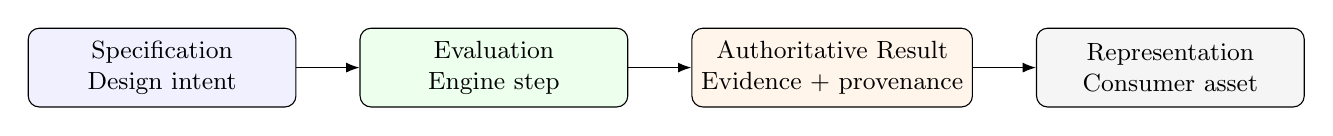
\begin{tikzpicture}[node distance=8mm,box/.style={draw,rounded corners,align=center,minimum width=34mm,minimum height=10mm,font=\small},a/.style={box,fill=blue!6},b/.style={box,fill=green!7},c/.style={box,fill=orange!8},d/.style={box,fill=gray!8}]
\node[a] (s) {Specification\\Design intent};
\node[b,right=of s] (e) {Evaluation\\Engine step};
\node[c,right=of e] (r) {Authoritative Result\\Evidence + provenance};
\node[d,right=of r] (p) {Representation\\Consumer asset};
\draw[-{Latex}] (s)--(e);
\draw[-{Latex}] (e)--(r);
\draw[-{Latex}] (r)--(p);
\end{tikzpicture}
\caption{The core semantic separation.}
\end{figure*}
\section{Rules}
\begin{itemize}[leftmargin=*,nosep]
\item Specifications store intent and references, not transient dirty state.
\item Evaluation is deterministic orchestration through the common Engine.
\item Results carry authoritative status, identity, topology/provenance and evidence.
\item Representations are derived and may be discarded/rebuilt without changing semantic truth.
\end{itemize}

\chapter{References, Topology, Coordinates, and Determinism}
\section{References}
References are first-class semantics. Required resolution states are Resolved, Missing, Ambiguous, Indeterminate, and Unsupported. Permanent array positions such as \texttt{Faces[12]} are forbidden as semantic identity.
\section{Topology evolution}
When an evaluation changes topology, it must produce explicit correspondence/evolution evidence. No downstream domain may guess a correspondence from visual similarity alone.
\section{Frames}
The architecture names World, Document, Part, Body, Sketch, Face, Occurrence, DrawingView and Simulation frames. Positive/negative feature direction is an oriented semantic extent; it is never inferred from viewer camera state.
\section{Determinism}
Evaluation identity contains normalized definition, resolved reference identities, parameters, expression identities, configuration/context, upstream result identities, tolerance policy, kernel contract version and representation policy as applicable. No object address, process-local hash, execution timestamp or viewer state.

\chapter{Cache, Incremental Recompute, and Representation Delta}
The architecture requires a single planner/evaluator path for full and incremental recomputation. Full recompute is maximal invalidation; incremental recompute is explicit change-set closure. Required invariants are:
\begin{lstlisting}[style=Prompt]
SemanticResult(FullRecompute(M, Delta)) == SemanticResult(IncrementalRecompute(M, Delta))
CacheHit(EvaluationIdentity) == FreshEvaluation(EvaluationIdentity)
\end{lstlisting}
Representation deltas derive from changed evaluation results and representation identities. Large assemblies must not regenerate unrelated render assets merely because one occurrence or one part changed.

\chapter{CATIA Capability Map - Functional Traceability}
This handbook treats CATIA as a capability reference, not an internal architecture to reproduce. The traceability chain is:
\begin{lstlisting}[style=Prompt]
External capability -> UMLCAD semantic capability -> services -> math contract -> authoritative result -> representation -> E2E evidence.
\end{lstlisting}
\section{Major families}
\begin{itemize}[leftmargin=*,nosep]
\item Part Design: extrusion/pad, pocket, revolution/shaft, groove, rib, slot, hole, shell, draft, fillet, chamfer, patterns, Boolean operations.
\item Sketch: support, geometry, constraints, solver state, publications.
\item Hybrid/GSD and Freeform: wireframe, surfaces, NURBS, matching, G0/G1/G2/G3, quality diagnostics, direct/associative editing, morphing.
\item Sheet Metal: thickness, bend, flange, relief, K-factor, tables, fold/unfold, flat pattern.
\item Product/Assembly: definitions, occurrences, transforms, configurations, constraints, engineering connections, BOM.
\item Kinematics: constraint equations, behavior, relations, motion state.
\item CAM: setup, stock, manufacturing features/operations, strategies, toolpaths, simulation, postprocessors, deterministic G-code/NC.
\item Drawing/PMI: projection, sections, details, clipping, dimensions, tolerances, GD\&T, annotations, dress-up, BOM, standards, DXF/DWG.
\item Knowledge/Configuration/Templates/Lifecycle/Integration: formulas, checks, reactions, reuse, variants, persistence, PLM/PDM/ERP integration.
\end{itemize}

\chapter{Independent-Agent Operating System}
\section{Branch isolation}
Every agent works in an isolated branch or worktree named after the chapter. Never share a working tree between agents for convenience. Merge only after the chapter gate and its evidence packet are complete.
\section{Contract-first synchronization}
Agents synchronize through repository artifacts: typed contracts, architecture manifest changes, test fixtures, evidence files, exact commit SHAs, and docs. No agent depends on another agent's private reasoning.
\section{No hidden coupling}
An agent that discovers a downstream need writes the required contract/evidence and records a blocker; it does not silently patch another agent's scope.
\section{Merge gates}
A receiving agent or integrator accepts a chapter only when architecture rules remain green, target tests execute, red-team cases pass, deterministic invariants hold, and no immutable scope was touched.
\section{Conflict strategy}
Prefer narrow files and contract boundaries. If two agents need the same semantic source file, split by contract/namespace first or serialize those changes rather than merging competing rewrites.

\chapter{Standalone Global Agent Charter}
The following charter is intentionally repeated conceptually inside every chapter prompt. An isolated agent should be able to reconstruct the same operating law without reading earlier chat history.
\begin{lstlisting}[style=Prompt]
ROLE: isolated UMLCAD.V.7 implementation agent.
REFERENCE SNAPSHOT: 7e0b143b182735c9dbc38a275043d32df7776650.
READ: the chapter's listed governing docs and exact repository files.
DO: inspect -> define authoritative RED -> classify boundary -> implement smallest complete path -> test -> red-team -> E2E -> record evidence.
NEVER: change frozen kernel/math/OCCT for an application-layer problem; duplicate geometry math; use topology array indices; turn viewer data into engineering truth; hide ambiguity; bypass Engine; make projects/demo canonical without a dedicated host milestone.
ALWAYS: preserve typed contracts, deterministic identities, explicit references/frames/tolerance, Specification/Evaluation/Result/Representation separation, full-vs-incremental equivalence, fail-closed invalid states.
HANDOFF: changed files, tests, evidence, architecture impact, unchanged assumptions, exact commit SHA, blockers, next safe boundary.
	extbf{Important}: no other agent's private knowledge exists. The repository is the shared memory.
\end{lstlisting}

\chapter{Chapter-to-Agent Assignment and Safe Parallel Waves}
\begin{tabularx}{\columnwidth}{@{}lX@{}}
\toprule
Wave & Chapters / purpose\\
\midrule
0 & 1-6 architecture/C4 and 7 frozen-boundary audit.\\
1 & 8-9 coding/testing law plus 10-25 kernel audits and contract inventory.\\
2 & 26-32 Expressions, Science, Semantics, Contracts, Engine, Kernel Client, legacy runtime boundary.\\
3 & 33-39 Resources, Sheet Metal, CAM, Drawing, Simulation, Viewer, Application Host.\\
4 & 40 S1 production slice, 41 CATIA traceability, 42-44 agent operating system and milestone closure.\\
\bottomrule
\end{tabularx}
\section{Parallelism condition}
Parallel waves may run concurrently only when they consume stable contracts and do not share mutable implementation files. The integrator serializes contract changes that multiple agents depend upon.
\section{Safe dependency examples}
Drawing may design against a published AuthoritativeCadResult contract without depending on a private Part Design implementation. CAM may consume a published FlatPatternResult without depending on private Sheet Metal classes. A kernel audit agent and a viewer agent may run concurrently because neither owns the other's semantic implementation.

\chapter{Definition of Done - Universal}
A capability is complete only when all applicable items are true:
\begin{enumerate}[leftmargin=*,nosep]
\item Semantic contract and ownership are explicit.
\item Implementation is inside the correct layer/domain.
\item Required mathematical contract is explicit and uses the frozen authority when available.
\item References, frames, configuration/context and tolerance semantics are deterministic.
\item Evaluation identity is complete and cache-safe.
\item Full and incremental paths are equivalent.
\item Authoritative result contains evidence/provenance; representation is derived.
\item Unit/contract/adapter tests execute.
\item Red-team, metamorphic, property/differential tests apply and pass.
\item Python E2E passes for the system workflow.
\item Full applicable repository gates pass on the exact commit.
\item Documentation records exact evidence and immutable boundaries.
\end{enumerate}
\section{Failure rule}
Unsupported, ambiguous, singular, stale, malformed, non-finite or otherwise unverifiable engineering state must produce structured failure. It must never be converted into plausible output merely to obtain a green test.

\chapter{Final Non-Negotiable Rules}
\begin{enumerate}[leftmargin=*,nosep]
\item .NET owns CAD meaning; Rust owns contracted mathematical authority.
\item OCCT is backend/oracle/wrapping infrastructure, not semantic authority.
\item The Engine is the execution center for system-CAD evaluation.
\item Specification, Evaluation, Result and Representation remain separate.
\item References are explicit and topology evolution is evidence-backed.
\item Viewer is presentation only.
\item Full and incremental recompute share one semantic/evaluation model.
\item Cache identity is deterministic and outside the kernel.
\item Exact circles are never replaced with polygonal proxies for authoritative S1 geometry.
\item CAM ends at deterministic postprocessed NC/G-code, not merely a visual toolpath.
\item Phenomena Simulation is a reusable scientific service with multiple providers.
\item Drawing consumes CAD authority and Science measurements; it never becomes geometry authority.
\item Product/Assembly/BOM semantics remain in CAD Core; consumers derive views.
\item Multiple agents communicate through repo artifacts, not private chat memory.
\item A milestone is GREEN only when every applicable gate executes and passes on the exact head.
\end{enumerate}
\backmatter
\chapter*{Closing note}
\addcontentsline{toc}{chapter}{Closing note}
This handbook is intentionally written as a system of independent execution packets. A capable coding agent can start with one chapter, read its listed sources, execute its prompt, and hand back evidence without needing the history of the other agents. The repository architecture, contracts and tests remain the common ground.
\end{document}
